\documentclass[final,letterpaper,twoside,12pt]{report}
\usepackage[vietnamese]{babel}
\usepackage{minitoc}
\usepackage{fix-cm}
\usepackage{amsfonts}
\usepackage{amsthm}
\usepackage{amsmath}
\usepackage{array}
\usepackage[utf8]{inputenc}
\usepackage[usenames,dvipsnames,table]{xcolor}
\usepackage{tikz}
\usepackage[framemethod=TikZ]{mdframed}
\mdfsetup{skipabove=\topskip,skipbelow=\topskip}
\usepackage{enumerate}
\usepackage{subcaption}
\usepackage{enumitem}
\setlist[enumerate]{topsep=0pt, itemsep=.5ex, parsep=ex}
\usepackage{tkz-tab}
\usepackage{subcaption}
\usepackage{float}
\usepackage{tcolorbox}
\renewcommand{\theequation}{\arabic{equation}}
\usepackage{tabularx}
\usepackage{amsmath}
\usepackage{amsthm}
\usepackage[colorlinks=true,urlcolor=red]{hyperref}
\usepackage{mdframed}
\usepackage{upgreek} 
\usepackage{algorithm}
\usetikzlibrary{decorations.pathreplacing}
\usepackage{algpseudocode}
\definecolor{venetianred}{rgb}{0.78, 0.03, 0.08}	
\definecolor{trueblue}{rgb}{0.0, 0.45, 0.81}
\definecolor{internationalorange}{rgb}{1.0, 0.31, 0.0}
\definecolor{persianred}{rgb}{0.0, 0.65, 0.58}
\definecolor{sapphire}{rgb}{0.03, 0.15, 0.4}
\definecolor{royalfuchsia}{rgb}{0.79, 0.17, 0.57}
\definecolor{azure(colorwheel)}{rgb}{0.0, 0.5, 1.0}
\usepackage{sectsty}
\chapterfont{\color{venetianred}}  
\sectionfont{\color{trueblue}}
\usepackage[left=2cm,right=2cm,top=3.5cm,bottom=3.54cm,headheight=1cm]{geometry}
\usepackage{pdfpages}
\usepackage{lipsum} 
\usepackage{multicol} 
\usepackage{amssymb}       
\usepackage{fontawesome5} 
\usepackage{listings}
\usetikzlibrary{shapes.geometric}

\definecolor{codebg}{rgb}{1.0,1.0,0.95}
\definecolor{commentgreen}{rgb}{0,0.6,0}
\definecolor{stringpurple}{rgb}{1,0,1}
\definecolor{linenumbergray}{gray}{0.4}
\definecolor{keywordred}{rgb}{0.8,0.0,0.0}

\lstset{
    language=Python,
    backgroundcolor=\color{codebg},
    basicstyle=\ttfamily\small,
    keywordstyle=\color{keywordred}\bfseries,
    stringstyle=\color{stringpurple},
    commentstyle=\color{commentgreen}\itshape,
    numberstyle=\tiny\color{linenumbergray},
    numbers=left,
    numbersep=10pt,
    frame=single,
    showstringspaces=false,
    breaklines=true,
    linewidth=1\textwidth,
	tabsize=2
}

\newmdenv[skipabove=7pt,
skipbelow=7pt,
rightline=false,
leftline=false,
topline=false,
bottomline=false,
innerleftmargin=5pt,
innerrightmargin=5pt,
innertopmargin=5pt,
leftmargin=0cm,
rightmargin=0cm,
linewidth=4pt,
innerbottommargin=5pt]{TDZ}

\geometry{
	paper=a4paper,
	inner=2.5cm,
	outer=2.5cm,
	bindingoffset=.5cm, 
	top=2cm,
	bottom=2.5cm,
}
\usepackage{fancyhdr}
\rfoot{Page \thepage}
\pagestyle{fancy}
\fancyhf{}
\rfoot{Trang \thepage}
\renewcommand{\footrulewidth}{0.8pt}
\lfoot{HCMUS}
\usepackage{environ}
\setlength{\parskip}{0.5em}
\setlength{\parindent}{0pt}
\allowdisplaybreaks
\newcommand{\blackbox}{\rule{0.17cm}{0.17cm}}

\begin{document}
\title{\bf \color{azure(colorwheel)} \Huge LEARN AI}
\date{}
\author{ \textbf{TTT}\\\textbf{22TNT}\\\textbf{HCMUS}\\\href{mailto:tongtrongtam1909@gmail.com?subject=Inbox}{tongtrongtam1909@gmail.com}}
\maketitle

\dominitoc
\tableofcontents


\part{ML(Machine Learning)}
\setcounter{chapter}{0}

\chapter{Linear regression}

\begin{itemize}
	\item Hồi quy tuyến tính là mô hình giả định mối quan hệ giữa đầu vào và đầu ra có thể được biểu diễn dưới dạng một đường thẳng, từ đó dự đoán các giá trị đầu vào chưa có nhãn.
	\item Nói cách khác, bài toán đang cố tìm một hàm tuyến tính:
	      $$
		      y = \beta_0 + \beta_1x_1 + \beta_2x_2 + \cdots + \beta_nx_n + \epsilon
	      $$
	      Trong đó:
	      \begin{itemize}
		      \item $\beta_i$, với $i = 0, 1, 2, \dots, n$, là các trọng số (weights).
		      \item $\epsilon$ là nhiễu (error term).
	      \end{itemize}
	\item Phương trình hồi quy tuyến tính:
	      $$
		      \hat{y} = \hat{\beta_0} + \hat{\beta_1}x_1 + \hat{\beta_2}x_2 + \cdots + \hat{\beta_n}x_n
	      $$
	\item Biểu diễn ma trận:
	      \begin{center}
		      \begin{tabular}{cccc}
			      $A = \begin{bmatrix}
					           1      & x_1^{(1)} & x_2^{(1)} & \cdots & x_n^{(1)} \\
					           1      & x_1^{(2)} & x_2^{(2)} & \cdots & x_n^{(2)} \\
					           1      & x_1^{(3)} & x_2^{(3)} & \cdots & x_n^{(3)} \\
					           \vdots & \vdots    & \vdots    & \ddots             \\
					           1      & x_1^{(m)} & x_2^{(m)} & \cdots & x_n^{(m)}
				           \end{bmatrix}$                                  &
			      $W = \begin{bmatrix}
					           \hat{\beta_0} \\ \hat{\beta_1} \\ \hat{\beta_2} \\ \vdots \\ \hat{\beta_n}
				           \end{bmatrix}$              &
			      $\hat{Y} = \begin{bmatrix} \hat{y}_1 \\ \hat{y}_2 \\ \vdots \\ \hat{y}_m \end{bmatrix}$ &
			      $Y = \begin{bmatrix} y_1 \\ y_2 \\ \vdots \\ y_m \end{bmatrix}$
		      \end{tabular}
	      \end{center}
	      $$\Rightarrow \hat{Y} \approx AW$$
	\item Hàm mất mát Mean-Squared Error (MSE):
	      $$
		      MSE = \dfrac{1}{m} \sum_{i=1}^m(\hat{y}_i - y_i)^2
	      $$
	      $$
		      \mathbf{W} = \arg \min_W(MSE)
	      $$
	\item Biến đổi MSE về dạng đại số:
	      \begin{align*}
		      MSE & = \dfrac{1}{m} \| AW - Y \|^2               \\
		          & = \dfrac{1}{m} (AW - Y)^T(AW - Y)           \\
		          & = \dfrac{1}{m} (W^TA^TAW - 2W^TA^TY + Y^TY)
	      \end{align*}
	\item Gradient:
	      \begin{align*}
		      \nabla MSE   & = \dfrac{2}{m}(A^TAW - A^TY)                                        \\
		      \nabla^2 MSE & = \dfrac{2}{m}A^TA > 0 \Rightarrow MSE \text{ có cực tiểu duy nhất}
	      \end{align*}
	\item Giải nghiệm tối ưu:
	      $$
		      W = (A^TA)^{-1}A^TY
	      $$
	\item Ví dụ: Dữ liệu số bóng bán dẫn (N) theo thời gian:

	      \begin{table}[H]
		      \centering
		      \begin{tabular}{|c|c|}
			      \hline
			      \textbf{Năm} & \textbf{Số bóng bán dẫn} \\
			      \hline
			      1971         & 2,250                    \\
			      1972         & 2,500                    \\
			      1974         & 5,000                    \\
			      1978         & 29,000                   \\
			      1982         & 120,000                  \\
			      1985         & 275,000                  \\
			      1989         & 1,180,000                \\
			      1993         & 3,100,000                \\
			      1997         & 7,500,000                \\
			      1999         & 24,000,000               \\
			      2000         & 42,000,000               \\
			      2002         & 220,000,000              \\
			      2003         & 410,000,000              \\
			      \hline
		      \end{tabular}
		      \caption{Dữ liệu số bóng bán dẫn theo thời gian}
		      \label{tab:transistor_table}
	      \end{table}

	      \begin{figure}[H]
		      \centering
		      
\includegraphics[width=0.8\textwidth]{transistors-per-microprocessor.png}
		      \caption{Số bóng bán dẫn theo thời gian trong các bộ vi xử lý}
	      \end{figure}

	\item a) Mô hình hoá: \( \log_{10}(N) \approx \theta_1 + \theta_2(t - 1970) \)
	\item b) Ước lượng bằng bình phương tối thiểu:
	      \begin{align*}
		      A             & = \begin{bmatrix} 1 & t - 1970 \end{bmatrix}, \quad Y = \begin{bmatrix} \log_{10}(N) \end{bmatrix}, \quad W = \begin{bmatrix} \theta_1 \\ \theta_2 \end{bmatrix} \\
		      \Rightarrow W & = (A^TA)^{-1}A^TY \approx \begin{bmatrix} 3.126 \\ 0.154 \end{bmatrix}
	      \end{align*}
	\item Dự đoán năm 2015:
	      \begin{align*}
		      \log_{10}(N)  & = 3.126 + 0.154(2015 - 1970) = 10.06      \\
		      \Rightarrow N & \approx 10^{10.06} = 1.137 \times 10^{10}
	      \end{align*}
	\item Sai lệch so với thực tế: \( \left|4 \times 10^9 - 1.137 \times 10^{10}\right| = 7.37 \times 10^9 \)

	\item \textbf{Nhận xét:} Mô hình tuyến tính trong thang đo log giúp dự đoán hợp lý, nhưng sai số lớn khi biến đổi ngược về giá trị gốc do bản chất phi tuyến trong tăng trưởng bóng bán dẫn.
\end{itemize}


\chapter{Gradient descent}

\begin{itemize}
	\item \textbf{Gradient Descent} là một thuật toán tối ưu hóa được sử dụng để tìm giá trị tối ưu (minima hoặc maxima) của một hàm. Trong học máy, phương pháp này chủ yếu được sử dụng để tối ưu hóa các tham số của mô hình (ví dụ: trọng số trong mạng nơ-ron).

	\item \textbf{Định nghĩa:} Gradient Descent là một phương pháp lặp đi lặp lại, trong đó các tham số (\(\theta\)) của mô hình được cập nhật theo hướng đối diện với gradient của hàm mất mát (loss function) tại mỗi bước, với mục tiêu giảm thiểu giá trị của hàm mất mát.

	\item \textbf{Công thức cập nhật tham số:} Ở mỗi bước \(i\), tham số được cập nhật theo công thức:
	      $$
		      \theta = \theta - \eta \nabla_\theta J(\theta)
	      $$
	      Trong đó:
	      \begin{itemize}
		      \item \(\theta\): Các tham số cần tối ưu hóa (ví dụ: trọng số của mô hình).
		      \item \(\eta\): Tốc độ học (learning rate), điều chỉnh độ lớn của mỗi bước cập nhật.
		      \item \(\nabla_\theta J(\theta)\): Gradient (đạo hàm) của hàm mất mát \(J(\theta)\) đối với tham số \(\theta\).
	      \end{itemize}

	\item \textbf{Vấn đề hội tụ:} Gradient Descent không thể tìm ra giá trị tối ưu chính xác mà chỉ có thể đạt đến một giá trị xấp xỉ. Do đó, thuật toán dừng lại khi sự thay đổi của tham số giữa các bước lặp là rất nhỏ, và không thay đổi đáng kể nữa. Chúng ta thường đặt một ngưỡng \(\epsilon\) để xác định khi nào thuật toán dừng lại. Điều này được biểu diễn bằng điều kiện:
	      $$
		      \left|\theta^{(i+1)} - \theta^{(i)}\right| < \epsilon
	      $$
	      Trong đó:
	      \begin{itemize}
		      \item \(\epsilon\) là ngưỡng dừng, giá trị nhỏ để đảm bảo thuật toán dừng khi sự thay đổi là không đáng kể.
	      \end{itemize}

	      \newpage

	\item \textbf{Tóm tắt thuật toán Gradient Descent:}
\end{itemize}

\begin{algorithm}
	\caption{Gradient Descent Algorithm}
	\begin{algorithmic}[1]
		\State \textbf{Input:} Data, learning rate \(\eta\), stopping threshold \(\epsilon\)
		\State \textbf{Initialize:} Choose initial values for the parameters \(\theta^{(0)}\)
		\Repeat
		\State Compute the gradient: \(\nabla_\theta J(\theta)\)
		\State Update the parameters: \(\theta^{(i+1)} = \theta^{(i)} - \eta \nabla_\theta J(\theta)\)
		\State Check stopping condition: \(\left|\theta^{(i+1)} - \theta^{(i)}\right| < \epsilon\)
		\Until{Stopping condition is satisfied}
		\State \textbf{Output:} Optimized parameters \(\theta\)
	\end{algorithmic}
\end{algorithm}


\chapter{Computational Graph}


\begin{itemize}
	\item \textbf{Computational Graph} (Đồ thị tính toán) là một công cụ được sử dụng để mô tả các phép toán toán học trong các mô hình học máy. Đồ thị này giúp mô tả cách dữ liệu và các phép toán di chuyển qua lại trong mô hình, từ đó dễ dàng tính toán gradient, tối ưu hóa tham số và gỡ lỗi mô hình.

	\item Computational Graph là một đồ thị có hướng, trong đó:

	      \begin{itemize}
		      \item \textbf{Các đỉnh (nodes)} đại diện cho các phép toán hoặc các giá trị (biến hoặc tham số).

		      \item \textbf{Các cạnh (edges)} đại diện cho sự phụ thuộc giữa các phép toán hoặc giá trị. Cạnh từ một đỉnh này đến đỉnh khác thể hiện rằng kết quả của phép toán tại đỉnh đầu tiên là đầu vào cho phép toán tại đỉnh thứ hai.
	      \end{itemize}

	      \newpage

	\item Xét hàm số  $y = (c+d)\times (a+c) + \dfrac{e^b}{a+c} $

	      $\hspace{1cm}$Biểu diễn dạng đồ thị:

	      \begin{tikzpicture}
		      \centering
		      \node[circle, draw, minimum size=0.8cm, line width=0.4mm] at (0, 0) {\fontsize{15}{18}\selectfont \textbf{b}};
		      \node[circle, draw, minimum size=0.8cm, line width=0.4mm] at (0, 3) {\fontsize{15}{18}\selectfont \textbf{a}};
		      \node[circle, draw, minimum size=0.8cm, line width=0.4mm] at (0, 6) {\fontsize{15}{18}\selectfont \textbf{c}};
		      \node[circle, draw, minimum size=0.8cm, line width=0.4mm] at (0, 9) {\fontsize{15}{18}\selectfont \textbf{d}};

		      \node[circle, draw, minimum size=0.8cm, line width=0.4mm] at (3, 7.5) {\fontsize{15}{18}\selectfont \textbf{t}};
		      \node[circle, draw, minimum size=0.8cm, line width=0.4mm] at (3, 4.5) {\fontsize{15}{18}\selectfont \textbf{f}};
		      \node[circle, draw, minimum size=0.8cm, line width=0.4mm] at (3, 1.5) {\fontsize{15}{18}\selectfont \textbf{g}};

		      \node[circle, draw, minimum size=0.8cm, line width=0.4mm] at (6, 3) {\fontsize{15}{18}\selectfont \textbf{u}};
		      \node[circle, draw, minimum size=0.8cm, line width=0.4mm] at (6, 6) {\fontsize{15}{18}\selectfont \textbf{v}};

		      \node[circle, draw, minimum size=0.8cm, line width=0.4mm] at (9, 4.5) {\fontsize{15}{18}\selectfont \textbf{y}};

		      \node[align=center] at (-4,4.5) {\fontsize{15}{18}\selectfont a $\leftarrow $ ? \\ \\\fontsize{15}{18}\selectfont b $\leftarrow $ ? \\\\\fontsize{15}{18}\selectfont c $\leftarrow $ ? \\ \\\\\fontsize{15}{18}\selectfont d $\leftarrow $ ? \\\\\fontsize{15}{18}\selectfont t $\leftarrow $ $c+d$ \\\\\fontsize{15}{18}\selectfont f $\leftarrow $ $a+c$ \\\\\fontsize{15}{18}\selectfont g $\leftarrow $ $e^b$ \\\\\fontsize{15}{18}\selectfont v $\leftarrow $ $t \times f$ \\\\\fontsize{15}{18}\selectfont u $\leftarrow $ $\dfrac{g}{f}$  \\\\\fontsize{15}{18}\selectfont y $\leftarrow $ $u+v$};

		      \draw[->,>=latex, line width=0.5mm,color = blue] (0.4,0.2) -- (2.65,1.4);
		      \draw[->,>=latex, line width=0.5mm,color = blue] (0.4,3.2) -- (2.65,4.4);
		      \draw[->,>=latex, line width=0.5mm,color = blue] (0.4,6.2) -- (2.65,7.4);

		      \draw[->,>=latex, line width=0.5mm,color = blue] (0.4,5.8) -- (2.65,4.6);
		      \draw[->,>=latex, line width=0.5mm,color = blue] (0.4,8.8) -- (2.65,7.6);

		      \draw[->,>=latex, line width=0.5mm,color = blue] (3.4,1.6) -- (5.65,2.8);
		      \draw[->,>=latex, line width=0.5mm,color = blue] (3.4,4.6) -- (5.65,5.8);

		      \draw[->,>=latex, line width=0.5mm,color = blue] (3.4,7.3) -- (5.65,6.2);
		      \draw[->,>=latex, line width=0.5mm,color = blue] (3.4,4.3) -- (5.65,3.2);

		      \draw[->,>=latex, line width=0.5mm,color = blue] (6.4,3.2) -- (8.65,4.3);

		      \draw[->,>=latex, line width=0.5mm,color = blue] (6.4,5.8) -- (8.65,4.7);

	      \end{tikzpicture}
	\item  Một số công thức đạo hàm quan trọng:
	      \begin{table}[h]
		      \centering
		      \renewcommand{\arraystretch}{2}
		      \begin{tabular}{|c|c|}
			      \hline
			      f(x)                                            & $\dfrac{d f(x)}{dx}$           \\
			      \hline
			      $\ln{x}$                                        & $\dfrac{1}{x}$                 \\
			      \hline
			      $e^x$                                           & $e^x$                          \\
			      \hline
			      $\sigma(x) = \dfrac{1}{1+e^{-x}}$               & $\sigma(x)\times(1-\sigma(x))$ \\
			      \hline
			      $\tanh{x} = \dfrac{e^x - e^{-x}}{e^x + e^{-x}}$ & $1 - (\tanh{x})^2$             \\
			      \hline
			      $\text{ReLU}(x) = \max(0, x)$                   &
			      $\begin{cases}
					       1                     & \text{nếu } x > 0 \\
					       0                     & \text{nếu } x < 0 \\
					       \text{không xác định} & \text{nếu } x = 0
				       \end{cases}$                                       \\
			      \hline
		      \end{tabular}
	      \end{table}

	      \newpage
	\item Tính đạo hàm từng phần:

	      Xét hàm số ở trên $y = (c+d)\times (a+c) + \dfrac{e^b}{a+c} $

	      Cho $a = 1, b=2, c=-3 , d=2$ Tính $\dfrac{\partial y}{\partial a}$,$\dfrac{\partial y}{\partial b}$,$\dfrac{\partial c}{\partial a}$,$\dfrac{\partial y}{\partial d}$

	      \begin{tikzpicture}
		      \centering
		      \node[circle, draw, minimum size=0.8cm, line width=0.4mm] at (0, 0) {\fontsize{15}{18}\selectfont \textbf{b}};
		      \node[circle, draw, minimum size=0.8cm, line width=0.4mm] at (0, 3) {\fontsize{15}{18}\selectfont \textbf{a}};
		      \node[circle, draw, minimum size=0.8cm, line width=0.4mm] at (0, 6) {\fontsize{15}{18}\selectfont \textbf{c}};
		      \node[circle, draw, minimum size=0.8cm, line width=0.4mm] at (0, 9) {\fontsize{15}{18}\selectfont \textbf{d}};

		      \node[circle, draw, minimum size=0.8cm, line width=0.4mm] at (3, 7.5) {\fontsize{15}{18}\selectfont \textbf{t}};
		      \node[circle, draw, minimum size=0.8cm, line width=0.4mm] at (3, 4.5) {\fontsize{15}{18}\selectfont \textbf{f}};
		      \node[circle, draw, minimum size=0.8cm, line width=0.4mm] at (3, 1.5) {\fontsize{15}{18}\selectfont \textbf{g}};

		      \node[circle, draw, minimum size=0.8cm, line width=0.4mm] at (6, 3) {\fontsize{15}{18}\selectfont \textbf{u}};
		      \node[circle, draw, minimum size=0.8cm, line width=0.4mm] at (6, 6) {\fontsize{15}{18}\selectfont \textbf{v}};

		      \node[circle, draw, minimum size=0.8cm, line width=0.4mm] at (9, 4.5) {\fontsize{15}{18}\selectfont \textbf{y}};


		      \draw[->,>=latex, line width=0.5mm,color = blue] (0.4,0.2) -- (2.65,1.4);
		      \draw[->,>=latex, line width=0.5mm,color = blue] (0.4,3.2) -- (2.65,4.4);
		      \draw[->,>=latex, line width=0.5mm,color = blue] (0.4,6.2) -- (2.65,7.4);

		      \draw[->,>=latex, line width=0.5mm,color = blue] (0.4,5.8) -- (2.65,4.6);
		      \draw[->,>=latex, line width=0.5mm,color = blue] (0.4,8.8) -- (2.65,7.6);

		      \draw[->,>=latex, line width=0.5mm,color = blue] (3.4,1.6) -- (5.65,2.8);
		      \draw[->,>=latex, line width=0.5mm,color = blue] (3.4,4.6) -- (5.65,5.8);

		      \draw[->,>=latex, line width=0.5mm,color = blue] (3.4,7.3) -- (5.65,6.2);
		      \draw[->,>=latex, line width=0.5mm,color = blue] (3.4,4.3) -- (5.65,3.2);

		      \draw[->,>=latex, line width=0.5mm,color = blue] (6.4,3.2) -- (8.65,4.3);

		      \draw[->,>=latex, line width=0.5mm,color = blue] (6.4,5.8) -- (8.65,4.7);

		      \node[align=center] at (13,4.5) {\fontsize{15}{18}\selectfont a $= $ 1 \\ \\\fontsize{15}{18}\selectfont b $=$ 2 \\\\\fontsize{15}{18}\selectfont c $=$ -3 \\\\\fontsize{15}{18}\selectfont d $= $ 2 \\\\\fontsize{15}{18}\selectfont t $= $ $-1$ \\\\\fontsize{15}{18}\selectfont f $=$ $-2$ \\\\\fontsize{15}{18}\selectfont g $=$ $e^2$ \\\\\fontsize{15}{18}\selectfont v $= $ $2$ \\\\\fontsize{15}{18}\selectfont u $ = $ $\dfrac{-e^2}{2}$  \\\\\fontsize{15}{18}\selectfont y $= $ $\dfrac{-e^2}{2}+2$};

		      \node[] at (2, 8.75) {\color{red}$\dfrac{\partial t}{\partial d}  = 1$};
		      \node[] at (2, 5.75) {\color{red}$\dfrac{\partial f}{\partial c}  = 1$};
		      \node[] at (1.25, 7.15) {\color{red}$\dfrac{\partial t}{\partial c}  = 1$};
		      \node[] at (1.25, 4.15) {\color{red}$\dfrac{\partial f}{\partial a}  = 1$};
		      \node[] at (1.25, 1.15) {\color{red}$\dfrac{\partial g}{\partial b}  = e^2$};
		      \node[] at (5.1, 7.25) {\color{red}$\dfrac{\partial v}{\partial t}  = -2$};
		      \node[] at (5.35, 4.25) {\color{red}$\dfrac{\partial u}{\partial f}  = \dfrac{-e^2}{4}$};
		      \node[] at (4.5, 5.75) {\color{red}$\dfrac{\partial v}{\partial f}  = -1$};
		      \node[] at (4, 2.65) {\color{red}$\dfrac{\partial u}{\partial g}  = \dfrac{-1}{2}$};
		      \node[] at (8, 5.75) {\color{red}$\dfrac{\partial y}{\partial v}  = 1$};
		      \node[] at (7.25, 4.) {\color{red}$\dfrac{\partial y}{\partial u}  = 1$};
	      \end{tikzpicture}

	      \begin{table}[h]
		      \centering
		      \renewcommand{\arraystretch}{2}
		      \begin{tabular}{|p{0.5cm}|p{8cm}|p{2cm}|}
			      \hline
			                                       & \textbf{Đạo hàm tiến}                                                                                                                                                                                                                                                                                  & Kết quả             \\
			      \hline
			      $\dfrac{\partial y}{\partial a}$ & $\dfrac{\partial a }{\partial a} \times \dfrac{\partial f}{\partial a} \times \dfrac{\partial v}{\partial f} \times \dfrac{\partial y}{\partial v} +\dfrac{\partial a}{\partial a} \times \dfrac{\partial f}{\partial a} \times \dfrac{\partial u}{\partial f} \times \dfrac{\partial y}{\partial u} $ & $\dfrac{-e^2}{4}-1$ \\
			      \hline
			      $\dfrac{\partial y}{\partial b}$ & $\dfrac{\partial b }{\partial b} \times \dfrac{\partial g}{\partial b} \times \dfrac{\partial u}{\partial g} \times \dfrac{\partial y}{\partial u} $                                                                                                                                                   & $\dfrac{-e^2}{2}$   \\
			      \hline
			      $\dfrac{\partial y}{\partial c}$ & $\dfrac{\partial c}{\partial c} \times \dfrac{\partial f}{\partial c} \times \dfrac{\partial v}{\partial f} \times \dfrac{\partial y}{\partial v} +\dfrac{\partial c}{\partial c} \times \dfrac{\partial t}{\partial c} \times \dfrac{\partial v}{\partial t} \times \dfrac{\partial y}{\partial v}$   & $-3$                \\
			      \hline
			      $\dfrac{\partial y}{\partial d}$ & $\dfrac{\partial d }{\partial d} \times \dfrac{\partial t}{\partial d} \times \dfrac{\partial v}{\partial t} \times \dfrac{\partial y}{\partial v} $                                                                                                                                                   & -2                  \\
			      \hline
		      \end{tabular}
	      \end{table}

	      Đạo hàm lùi làm tương tự, kết quả vẫn như đạo hàm tiến.
\end{itemize}


\part{DL(Deep Learning)}
\setcounter{chapter}{0}

\part{NLP(Natural Language Processing)}
\setcounter{chapter}{0}

\chapter{Thuật toán tách từ}

Slide: token.pdf

\section{Byte-Pair Encoding BPE(gpt dùng)}

link: \href{https://protonx.io/news/chi-tiet-thuat-toan-tach-token-byte-pair-encoding-bpe-1702295274898}{here}.

\section{WordPiece(BERT dùng)}

Tương tự như thuật toán trên nhưng:

BPE chỉ là đếm số lượng còn với WP thì sẽ chia số số lần xuất hiện để chuẩn hóa lại

vd:  $\dfrac{\textbf{số lần xuất hiện am}}{\textbf{số lần xuất hiện a * só lần xuất hiện m}}$

mục đích: hạn chế việc các từ đơn lẻ xuất hiện quá nhiều

WP còn dùng cặp thăng để nối các token lại

\texttt{['[CLS]', 'i', 'am', 'study', '\#\#ing', 'math', '[SEP]']}

$\longrightarrow$ I am studying math.

\chapter{Chuẩn hóa văn bản}

Chuẩn hóa văn bản là một chuỗi việc \textbf{chuyển văn bản sang dạng chuẩn, thuân tiện }để sử dụng trong các bài toán khác nhau

Slide: text normalization.pdf

\textbf{Stanza }\href{https://stanfordnlp.github.io/stanza/index.html}{here}
\subsection{Tách câu(Sentence segmentation)}

Chia văn bản thành các câu

\subsection{Tách token(tokenization)}

$\bullet$ Chia văn bản thành các token

$\bullet$ Việc chia này dựa vào dấu câu như (.) ,(?) , (!). Vấn đề khó khăn xảy như như trong từ viết tắt của Tiếng Ánh như Mr. Mrs. thì (.) này không phải là kết của 1 câu.


\subsection{Lemmatizaion}
$\bullet$ 9 cách sử dụng lemmatization : \href{https://www.geeksforgeeks.org/python-lemmatization-approaches-with-examples/}{here}

$\bullet$ Lemmatization là task xác định hai từ có cùng gốc. Chúng ta sẽ xây dựng một lemmatizer mapping tất cả các từ này về nguyên bản.

vd: buys, bought, buying $\rightarrow$ buy

$\bullet$ Mục tiêu: thu gọn không gian phân tích, tạo ra độ chính xác cao hơn


$\bullet$ Nhược điểm: Nếu bộ dữ liệu có sự mập mờ lớn thì việc xử lý này sẽ đánh mất đi thông tin về ngữ nghĩa, ngữ pháp giảm độ chính xác của mô hình.

Vd: có thể là 1 câu mỉa mai bảo nhiều nma thật ra lại là ít.

$\bullet$ Thực hành lemma

$\hspace*{0.5cm} \circ$ \textbf{Natural language toolkit: } \href{https://www.nltk.org/}{here} (dùng nhiều)

$\hspace*{0.5cm} \circ$\ \textbf{spaCy: }\href{https://spacy.io/}{here} (dùng nhiều nhất)  Kiến trúc Spacy : \href{https://spacy.io/usage/spacy-101#architecture}{here}

$\hspace*{0.5cm} \circ$\ \textbf{TextBlob: }\href{https://textblob.readthedocs.io/en/dev/}{here}.

$\hspace*{0.5cm} \circ$\ \textbf{Standford coreNLP: }\href{https://textblob.readthedocs.io/en/dev/}{here}.

\subsection{Stemming}

$\bullet$ Cắt hậu tố khỏi từ, ít được sử dụng hơn lemmatization

Vd: buying cắt bỏ ing $\rightarrow$ buy

\subsection{Lọc stop words}

$\bullet$ Lọc những từ hay xuất hiện và ít ngữ nghĩa như "the", "is", "at","wich" và "on"

\subsection{Sửa sai từ(word correction) }
Cấu trúc dữ liệu trie:  \href{https://www.geeksforgeeks.org/trie-insert-and-search/}{here}

$\bullet$ Sai thứ tự từ trong Tiếng Anh hoặc sai dấu trong Tiếng Việt.

happpy $\longrightarrow$ happy

azmazing $\longrightarrow$ amazing

inteliggent $\longrightarrow$ intelligent
\subsubsection{Jaccard distance}

\textbf{dùng n- grams}

\textbf{ví dụ} với bigram:xét 2 từ hello với elhlo:

$\hspace*{0.5cm}\bullet$ hello $\rightarrow$ \{he,el,ll,lo\}

$\hspace*{0.5cm}\bullet$ hlleo $\rightarrow$ \{hl,ll,le,eo\}

$\hspace*{0.5cm}\bullet$ union  = \{ll\}

$\hspace*{0.5cm}\bullet$ intersection = \{he,el,ll,lo,hl,le,eo\}

$\Longrightarrow$Jaccard distance = $1- \dfrac{len(union)}{len(intersection)} = \dfrac{6}{7}$

\subsubsection{Edit distance}

Edit distance hay còn được gọi là Levenshtein  distance đo lường \textbf{\color{red}tổng số phép nhỏ nhất} cần thực hiện biến đổi chuỗi A thành chuỗi B

Số loại phép biến đổi bao gồm :

$\hspace*{0.5cm}\bullet$ Phép chèn (insertion)

$\hspace*{0.5cm}\bullet$ Phép xóa ( deletion)

$\hspace*{0.5cm}\bullet$ Phép thay thế (Substitution)

Ví dụ: kitten $\rightarrow$ sitting

$\Longrightarrow$ Edit distance = 3: cần ít nhất 3 phép để chuyển kitten thành sitting:

$\hspace*{0.5cm}\bullet$ thay k thành s (kitten $\rightarrow$ sitten)

$\hspace*{0.5cm}\bullet$ thay e thành i (sitten $\rightarrow$ sittin)

$\hspace*{0.5cm}\bullet$ thêm g ở cuối ( sittin $\rightarrow$ sitting)

\subsubsection{Quy trình sửa sai từ (word correction pipeline)}

\begin{center}
	\begin{tikzpicture}[scale=1.4,auto,swap]
		\node[draw, dashed] at (-2,0) (x) {\text{  từ     }};
		\node[draw, dashed] at (0,-3) (y) {\text{  từ điển    }};
		\node[draw, dashed] at (7,0) (z) {\text{  từ đúng    }};
		\node at (4,-1.5) {\parbox{9cm}{
				\textbf{\footnotesize {$\bullet$ lặp qua các từ trong từ điển}} \\
				\textbf{\footnotesize {$\bullet$ Tính khoảng cách của các từ này với từ mục tiêu}} \\
				\textbf{\footnotesize {$\bullet$ Từ nào trong từ điển có \textcolor{red}{khoảng cách ngắn nhất} thì đề xuất từ đó thay thế}}
			}};

		\draw[->,>=latex, line width=0.5mm,color = blue] (x) -- (z);
		\draw[->,>=latex, line width=0.5mm,color = blue] (y)--  (0,0);

	\end{tikzpicture}
\end{center}
\section{Bài toán}

$\bullet$ Chuẩn hóa văn bản \textbf{khác nhau} giữa các bài toán.

$\bullet$ Tùy bài toán khác nhau thì sẽ lựa chọn bộ chuẩn hóa, không phải cái nào cũng sài.

\subsection{Bài toán sinh từ(text Generation)}

$\bullet$ Giữ nhiều token nhất có thể, đưa các văn bản về chung một format.

Ví dụ: lùi đầu dòng, viết hoa đầu câu,..

\subsection{Bài toán phân loại cản xúc(Sentiment Classification)}

$\bullet$ Loại bỏ các stop words như a, to,...

$\bullet$ Giữ lại biểu tượng cảm xúc như :),:D,...

Data:

\begin{tabular}{|p{0.8\linewidth}|c|}
	\hline
	Text                                           & Sentiment \\
	\hline
	One of the other reviewers has mentioned that  & positive  \\\hline
	A wonderful little production. <br /><br />The & positive  \\\hline
	Basically there's a family where a little boy  & negative  \\\hline
\end{tabular}

\textbf{Pipeline}

\begin{tikzpicture}[scale=1.35,auto,swap]
	\node[draw] at (0,0) (x) {\textbf{csv file}};
	\node[draw] at (2.3,0) (y) {\textbf{cleaned text}};
	\node[draw] at (5.25,0) (z) {\textbf{tokenized matrix}};
	\node[draw] at (8.85,0) (t) {\textbf{classification model}};

	\draw[->,>=latex, line width=0.5mm,color = blue] (x) -- (y);
	\draw[->,>=latex, line width=0.5mm,color = blue] (y) -- (z);
	\draw[->,>=latex, line width=0.5mm,color = blue] (z) -- (t);
\end{tikzpicture}

\section{Làm việc với Tiếng Việt}
Một số lưu ý khi làm việc với Tiếng Việt:
\href{https://universaldependencies.org/vi/index.html}{here}

\subsection{spacy cho Tiếng Việt :}


\subsection{Thư viện underthesea}

$\bullet$ Bộ công cụ NLP tiếng Việt - Underthesea là một bộ công cụ bằng ngôn ngữ Python mã nguồn mở bao gồm các mô-đun, bộ dữ liệu và hướng dẫn hỗ trợ nghiên cứu và phát triển trong lĩnh vực Xử lý Ngôn ngữ Tự nhiên tiếng Việt. Thư viện có các API dễ sử dụng để nhanh chóng áp dụng các mô hình NLP tiền huấn luyện cho văn bản tiếng Việt của bạn, như phân đoạn từ (Word segmentation), gán phần loại từ (PoS), nhận diện thực thể đặt tên (Named entity recognition - NER), phân loại văn bản (Text Classification) và phân tích phụ thuộc (Dependency Parsing).

$\bullet$ Chi tiết \href{https://github.com/undertheseanlp/underthesea}{here}

$\bullet$ \textbf{Tách văn bản thành các câu}



$\bullet$ \textbf{Chuẩn hóa văn bản}

Vị trí dấu được điều chỉnh phù hợp.

$\bullet$ \textbf{Tách câu thành từ}


$\bullet$ \textbf{POS Tagging - Đánh nhãn từ}


$\bullet$ \textbf{Phân tích cảm xúc câu}



\chapter{Các thuật toán traning}

\section{Stochastic gradient descent(SGD)}

$\bullet$Sử dụng quán tính mô hình có khả năng hội tụ nhanh hơn và vượt qua các điểm \textbf{\color{red}cực tiểu cục bộ (yên ngựa)}

$\bullet$Công thức quán tính ( Momentum):

$\hspace*{0.5cm} \circ$ $\theta_{t+1} = \theta_t - v_t$

$\hspace*{0.5cm} \circ$ $v_t = \gamma v_{t-1} +\alpha \bigtriangledown J(\theta_{t})$ $(v_0 = 0 \rightarrow v_1 = \alpha \bigtriangledown J(\theta_{1}))$


\section{Adagrad}
Tài liệu \href{https://d2l.aivivn.com/chapter_optimization/adagrad_vn.ht}{here} và \href{https://optimization.cbe.cornell.edu/index.php?title=AdaGrad}{here}

vấn đề của quán tính là càng ngày càng được tích tụ dẫn tới việc tối ưu vược khỏi điểm cực trị.

$\bullet$ \textbf{\color{red}Adagrad} có khả năng điều chỉnh tốc độ học dụa vào tham số

$\bullet$ Thực hiện cập nhật:

$\hspace*{0.5cm}\circ$ \textbf{\color{red}Ít} với tham số liên quan đếm features thường xuyên xuất hiện \textbf{\color{red}(tốc độ học giảm)}

$\hspace*{0.5cm}\circ$ \textbf{\color{red}Nhiều} với tham số liên quan đếm features ít xuất hiện \textbf{\color{red}(tốc độ học lớn)}

$\rightarrow$ phù hợp với dữ liệu thưa

$\bullet$\textbf{\color{red}Adagrad} sử dụng tốc độ học khác nhau cho những tham số khác nhau ở một \textbf{timestep t}.

Khi Gradient lớn, tốc độ học giảm, khi Gradient nhỏ, tốc độ học tăng.

$$\theta_{t+1} = \theta_t - \dfrac{\alpha}{\sqrt{G_t+\epsilon}}\odot \bigtriangledown J(\theta)$$

Tổng dồn bình phương Gradient \textbf{\color{red}từ đầu} đến \textbf{\color{red}timestep t hiện tại}
\[
	G_t = \sum_{j=1}^{t} G_j \odot G_j = \sum_{j=1}^{t} \bigtriangledown J(\theta_j) \odot\bigtriangledown J(\theta_j)
\]

\[
	\theta_t \in \mathbf{R}^{d\times d}   \hspace*{0.5cm} G_t \in \mathbf{R}^{d \times d }
\]

$\bullet$ Điểm mạnh: Xóa bỏ việc điều chỉnh tốc độ học bằng tay

$\bullet$ Điểm yếu: $G_t$ đặt ở dưới thương. Được cộng dồn từ đầu tới mỗi timestep t nhất định, khả năng cao mẫu rất lớn khiến tốc độ học giảm xuống xấp xỉ 0, dẫn tới mô hình \textbf{\color{red}không học được thông tin mới}. Để khác phục điều này ta tới tiếp các một số thuật toán tiếp theo.

\subsection{Adadelta}

$\bullet$ \textbf{\color{red}Adadelta} sẽ khác phục vấn đề của \textbf{\color{red}Adagrad}, vấn đề tốc độ học sẽ chạm tới khi khi timestep đủ lớn.

$\bullet$ Thay vì tính tổng dồn bình phương gradient \textbf{từ đầu} đến \textbf{timestep t } hiện tại, Adadelta chỉ tính tổng dồn w lần gradient tới thời điểm hiện tại.

$\bullet$ Thay vì sử dụng w chúng ta sẽ thực hiện như sau:
$$g_t = \bigtriangledown J(\theta_t)$$

$$E[g^2]_t = \gamma E[g^2]_{t-1} + (1 - \gamma)g^2_t $$

Tương tự như momentum: $\gamma = 0.9$

$$\theta_{t+1} = \theta_t - \dfrac{\alpha}{\sqrt{E[g^2]_t + \epsilon}}g_t$$

$\longrightarrow$ Thay vì sử dụng một learning rate cố định, Adadelta sử dụng một phương pháp điều chỉnh learning rate dựa trên tỷ lệ của các bước cập nhật trước đó. Điều này có nghĩa là khi các tham số càng xa thì bước cập nhật sẽ được điều chỉnh tự động để phù hợp với mức độ cần thiết.$\theta_t$ chỉ quan tới tới các $\theta$ ở gần nó mà thôi.


$\bullet$ \textbf{Thuật toán RMSprop} Tương tự như Adadelta nhưng chưa được công bố.

\section{Adam (Adaptive Moment Estimation)}

Tài liệu: \href{https://d2l.aivivn.com/chapter_optimization/adam_vn.html#lap-trinh}{here}

$\bullet$ \textbf{\color{red}Adam} ngoài việc lưu lại trung bình bình phương gradient trong quá khứ như \textbf{\color{red}Adadelta và RMSprop}, \textbf{\color{red}Adam} còn lưu lại trung bình giống \textbf{\color{red}Momentum}

$$m_t = \beta_1 m_{t-1} + (1 - \beta_1)g_t \Longrightarrow \text{Đo lường trung bình Gradient (Mean)}$$

$$v_t = \beta_2 v_{t-1} + (1 - \beta_2) g^2_t\Longrightarrow \text{Đo lường phương sai Gradient (Variance)}$$

Thời điểm ban đầu $m_0$ và $v_0$ bằng 0, mà $\beta_1$ và $\beta_2$ gần tới 1 dẫn tới $m_1$ và $v_1$ gần tới 0 ( bị bias tới 0). Cho nên tác giả quyết định xử lý vấn để này bằng cách:

\begin{center}
	\begin{tikzpicture}
		\node at (0,0) {$\hat{m}_t = \dfrac{m_t}{1-\beta_1^t}$};
		\node at (0,-1.5) {$\hat{v}_t = \dfrac{v_t}{1-\beta_2^t}$};
		\node[align=center] at (3.8,-0.5) (z) {\color{red}\small Tương tự Adadelta \\\color{red}\small và RMSprop};
		\node at (10,-1) {$\theta_{t+1} = \theta_t - \dfrac{\alpha}{\sqrt{\hat{v}_t}+\epsilon}\hat{m}_t $};
		\draw (2,0.5) -- (2,-2);
		\draw[->] (2,-1) -- (7,-1);
	\end{tikzpicture}
\end{center}

$\bullet$ Ở đây có 1 sự khác biệt thay vì dùng ${\sqrt{\hat{v}_t+\epsilon}}$ thì lại dùng ${\sqrt{\hat{v}_t}+\epsilon}$

$\bullet$ Ở đây  $\beta_!$ và  $\beta_2$ là các tham số trọng số không âm. Các lựa chọn phổ biến cho chúng là  $\beta_1=0.9$ và $\beta_2 = 0.999$


\chapter{Vector Semantics và Embeddings}

\section{Vector Semantics}

$\bullet$ Lexical semantics

Phân tích đại diện ngữ nghĩa trên đơn vị là \textbf{từ - word meaning} (nghiên cứu về ý nghĩa của một từ, và hệ thống kết nối ý nghĩa của một từ)

\begin{tikzpicture}
	\draw[thick] (0, 2) circle (0.25) node (a) {};
	\draw[thick] (3, 2) circle (0.25) node (b) {};
	\draw[thick] (6, 2) circle (0.25) node (c) {};
	\draw[thick] (9, 2) circle (0.25) node (d) {};
	\draw[thick] (12.5, 2) circle (0.25) node (e) {};

	\node[align=center] at (0,0) (z) {\tiny \textbf{Sự tương đồng về}  \\\tiny \textbf{ngữ nghĩa} \\\tiny  \textbf{(word similarity)} \\ \\ \tiny\textbf{Chó} và \textbf{mèo}};

	\node[align=center] at (3,0) (z) {\tiny \textbf{Từ đồng nghĩa}  \\\tiny \textbf{(Synonym)} \\ \\ \tiny\textbf{Hạnh phúc} và \\ \tiny \textbf{sung sướng}};

	\node[align=center] at (6,0.25) (z) {\tiny \textbf{Từ trái nghĩa}  \\\tiny \textbf{(Antonym)} \\ \\ \tiny\textbf{Ngắn} và \tiny\textbf{Dài}};

	\node[align=center] at (9,-0.4) (z) {\tiny \textbf{Hàm ý}  \\\tiny \textbf{tích cực/tiêu cực} \\\tiny  \textbf{(Positive/Negative }\\ \tiny  \textbf{Connotations)} \\ \\ \tiny\textbf{Hạnh phúc} và \\ \tiny \textbf{Đau khổ}};

	\node[align=center] at (12.5,-0.65) (z) {\tiny \textbf{Trường ngữ nghĩa}  \\\tiny \textbf{(Semantic Field)} \\ \\ \tiny  \textbf{(Marketting, kinh)}\\ \tiny\textbf{Doanh, chi phí, lợi} \\\tiny\textbf{nhuận} cùng thuộc \\\tiny trường nghĩa: \\\tiny\textbf{Kinh doanh}};

	\draw[->,>=latex, line width=0.5mm,color = red] (6,6) -- node[auto, scale=0.8] {} (a);
	\draw[->,>=latex, line width=0.5mm,color = red] (6,6) -- node[auto, scale=0.8] {} (b);
	\draw[->,>=latex, line width=0.5mm,color = red] (6,6) -- node[auto, scale=0.8] {} (c);
	\draw[->,>=latex, line width=0.5mm,color = red] (6,6) -- node[auto, scale=0.8] {} (d);
	\draw[->,>=latex, line width=0.5mm,color = red] (6,6) -- node[auto, scale=0.8] {} (e);
\end{tikzpicture}

$\circ$ Word similarity

Việc mở rộng phạm vi đánh giá 2 từ thay vì sử dụng mối quan hệ \textbf{Word senses}(đồng nghĩa, trái nghĩa) sang quan hệ tương đồng \textbf{(Word similarity)} làm \textbf{đơn giản độ phức tạp } của bài toán.

Simlex - 999 Data set ( khoảng từ 0 - 10)

\begin{center}
	\begin{tikzpicture}
		\node at (0,0) {
			\begin{tabular}{|c|c|c|}
				\hline
				achieve & accomplish & 8.57 \\ \hline
				accept  & reject     & 0.83 \\ \hline
				water   & ice        & 6.47 \\ \hline
			\end{tabular}
		};
		\node at (7,0.65) {\texttt{Đồng nghĩa}};
		\node at (7,0) {\texttt{Trái nghĩa}};
		\node at (8.75,-0.65) {\texttt{Có sự tương đồng ngữ nghĩa}};

		\draw[->] (5.25,0.6) -- (3,0.6);
		\draw[->] (5.25,0) -- (3,0);
		\draw[->] (5.25,-0.6) -- (3,-0.6);
	\end{tikzpicture}
\end{center}

\subsection{Vector ngữ nghĩa (Semantic vector)}

$\bullet$ Ngữ nghĩa của một từ được định nghĩa thông qua \textbf{Phân bố (distribution)} của nó trong việc sử dụng ngôn ngữ.

$\bullet$ Hai từ có cùng \textbf{phân bố (similar distribution - các từ xung quanh tương đồng nhau)} sẽ có ngữ nghĩa giống nhau

$\hspace*{0.5cm} \Longrightarrow$ Ý nghĩa của \textbf{Vector ngữ nghĩa} là biểu diễn cho một từ dưới dạng \textbf{không gian ngữ nghĩa nhiều chiều (multidimensional sematic space)}, không gian này được xây dựng dựa trên mối quan hệ với các từ xung quanh.

\section{Embeddings}

Mô phỏng từ bằng vector nhiều chiều, những từ tương đồng nhau thì vector sẽ gần nhau.

Word embedding được sử dụng để biểu diễn từ trước khi đưa vào mô hình NLP

$\bullet$ \textbf{Vector thưa(Sparse vector)}: Yếu trong việc mô tả tương đồng ngữ nghĩa, ví dụ 2 vector của từ "Gà" và "Đồng vật" có thể hoàn toàn khác nhau.

$\bullet$ \textbf{Vector dày(Dense vector)}:(E.g. 300 chiều) hoạt động tốt hơn Sparse vector(E.g. 10000 chiều) trong các NLP task vì Dense vector yêu cầu ít params hơn giảm test error(generation error) - \textbf{tránh overfitting}

$\bullet$ \textbf{One-hot vector: }là vector chứa duy nhất một phần tử là 1 còn tất cả là 0. Giá trị của từ trong từ điển sẽ
là vị trí của 1 trong vector. Chiều của one - hot vector bằng
số lượng từ trong từ điển

\begin{center}

	\begin{tikzpicture}
		\node at (0,2) {\texttt{Dense vector}};
		\node at (0,0)  {$\text{eat} = \begin{bmatrix}
					-0.2 \\0.1\\0.5\\2.8\\-1.7
				\end{bmatrix}$};

		\node at (4,2) {\texttt{Sparse vector}};
		\node at (4,-0.5) {$\text{eat} = \begin{bmatrix}
					0 \\20\\0\\3\\ \vdots\\ 0\\0
				\end{bmatrix}$};

		\node at (8,2) {\texttt{One-hot vector}};
		\node at (9,-0.5) {$\text{eat} = \begin{bmatrix}
					0 \\0\\1\\0\\ \vdots\\ 0\\0
				\end{bmatrix}$(dict['eat'] = 2)};

	\end{tikzpicture}
\end{center}

\subsection{Word2vec}

\textbf{Tài liệu}\href{https://arxiv.org/pdf/1411.2738v4}{here}

Word2Vec là một embedding tĩnh (static embedding), một từ
được biểu diễn dưới dạng một vector cố định (fixed
embedding)

Những Embedding tiên tiến hiện nay như BERT hoặc ELMO biểu
diễn từ dưới dạng vector ngữ cảnh động (dynamic contextual
embedding), tức là một từ sẽ có biểu diễn khác nhau trong
những ngữ cảnh khác nhau.



\subsection{Continuous Bag Of Words(CBOW)}

Giải thích toán: \href{https://www.youtube.com/watch?v=GMCwS7tS5ZM}{here}

Ý tưởng: dùng các từ ngữ phía trước và sau để dự đoán từ ở giữa. Ở đây sẽ dùng 2 từ trước và 2 từ sau

Ví dụ từ điển có 30 từ + OOV = 31

\begin{tikzpicture}
	\node at (0,0) {$\begin{bmatrix}
				0 \\1\\0\\ \vdots\\ 0\\0
			\end{bmatrix}$};
	\node at (0,4) {$\begin{bmatrix}
				0 \\1\\0\\ \vdots\\ 0\\0
			\end{bmatrix}$};
	\node at (0,8) {$\begin{bmatrix}
				0 \\1\\0\\ \vdots\\ 0\\0
			\end{bmatrix}$};
	\node at (0,12) {$\begin{bmatrix}
				0 \\1\\0\\ \vdots\\ 0\\0
			\end{bmatrix}$};

	\node at (0,-2.5) [align=center] {$\textbf{\textnormal{e}}_{i}$ \\ \textbf{i = $\overline{1,4}$} \\ \textbf{\color{red}[1$\times$31]}};

	\node at (3,0) {$\begin{bmatrix}
				\\\\\\ \vdots\\ \\
			\end{bmatrix}$};
	\node at (3,4) {$\begin{bmatrix}
				\\ \\ \\ \vdots\\  \\
			\end{bmatrix}$};
	\node at (3,8) {$\begin{bmatrix}
				\\\\\\ \vdots\\ \\
			\end{bmatrix}$};
	\node at (3,12) {$\begin{bmatrix}
				\\ \\ \\ \vdots\\ \\
			\end{bmatrix}$};

	\node at (3,-2.5) [align=center] {$\textbf{\textnormal{e}}_{i}^{'}$ \\ \textbf{i = $\overline{1,4}$} \\ \textbf{\textcolor{red}{[1$\times$300]}}};

	\draw[->,>=latex, line width=0.5mm,color = blue] (0.5,12) -- node[auto, scale=0.8] {} (2.75,12);
	\draw[->,>=latex, line width=0.5mm,color = blue] (0.5,8) -- node[auto, scale=0.8] {} (2.75,8);
	\draw[->,>=latex, line width=0.5mm,color = blue] (0.5,4) -- node[auto, scale=0.8] {} (2.75,4);
	\draw[->,>=latex, line width=0.5mm,color = blue] (0.5,0) -- node[auto, scale=0.8] {} (2.75,0);

	\node at (1.5,12.25) {\color{red}$\textnormal{e}_{1} \odot W_1$};
	\node at (1.5,8.25) {\color{red}$\textnormal{e}_{2} \odot W_1$};
	\node at (1.5,4.25) {\color{red}$\textnormal{e}_{3} \odot W_1$};
	\node at (1.5,0.25) {\color{red}$\textnormal{e}_{4} \odot W_1$};

	\node at (7,6) {$\begin{bmatrix}
				\\ \\ \\ \vdots\\ \\
			\end{bmatrix}$};

	\draw[->,>=latex, line width=0.5mm,color = blue] (3.25,12) -- node[auto, scale=0.8] {} (6.75,6);
	\draw[->,>=latex, line width=0.5mm,color = blue] (3.25,8) -- node[auto, scale=0.8] {} (6.75,6);
	\draw[->,>=latex, line width=0.5mm,color = blue] (3.25,4) -- node[auto, scale=0.8] {} (6.75,6);
	\draw[->,>=latex, line width=0.5mm,color = blue] (3.25,0) -- node[auto, scale=0.8] {} (6.75,6);

	\node at (7,3.5) [align=center]  {${\textnormal{e}} = \dfrac{1}{4}\displaystyle\sum_{i=1}^{4} \textnormal{e}_{i}^{'}$ \\ \color{red} [1$\times3$00]};
	\node at (11,6) {$\begin{bmatrix}
				\\ \\ \\ \vdots\\ \\
			\end{bmatrix}$};

	\draw[->,>=latex, line width=0.5mm,color = red] (7.25,6) -- node[auto, scale=0.8] {} (10.75,6);

	\node at (8.75,6.25) {\color{red}$\textnormal{e} \odot W_2$};
	\node at (11,4) [align=center] {$\hat{y}$ \\ {\color{red}[1$\times$31]}};

	\node at (14,6) {$\begin{bmatrix}
				\\ \\ \\ \vdots\\ \\
			\end{bmatrix}$};

	\node at (14,4) [align=center] {${y}$ \\ {\color{red}[1$\times$31]}};

	\node at (14,8) {\textbf{\textcolor{red}{\small One-hot  vector}}};
	\draw[<->,>=latex, line width=0.5mm,color = red] (11.25,5) -- node[auto, scale=0.8] {} (13.75,5);
	\draw[<->,>=latex, line width=0.5mm,color = red] (11.25,7) -- node[auto, scale=0.8] {} (13.75,7);
	\node at (12.5,6) {\textbf{\textcolor{red}{Loss}}};

	\node at (10,11) {\textbf{\color{red}$W_1$: [31 $\times$ 300]}};
	\node at (10,10) {\textbf{\color{red}$W_2$: [300 $\times$ 1]}};

	\node at (10,2) {\textbf{Từ hàm loss điều chỉnh các parameter của $W_1,W_2$}};

	\node at (10,1) {\color{red} $W_1$ được gọi là ma trận embedding};
	\node at (10,0) {{\color{red}$\textbf{\textnormal{e}}_{i}^{'}$ được gọi là vector embedding}};

\end{tikzpicture}

Với i là vị trí số 1 trong one-hot vector của 1 từ thì vector embedding của từ đó sẽ là hàng i của ma trận embedding.

\subsection{SkipGram}

Vấn đề của CBOW là khi từ điển quá lớn thì tốc độ sẽ chậm đi đáng kể, để khác phục điều này thì thuật toán SkipGram xuất hiện.

Ý tưởng: Ngược lại với CBOW, SkipGram dự đoán những từ xung quanh dựa vào 1 từ cho trước

\begin{tikzpicture}
	\node at (0,10) {\small \textbf{Input}};
	\node at (2.5,10) {\small \textbf{Projection}};
	\node at (5.25,10) {\small \textbf{Output}};

	\draw (-0.25,9.25) rectangle (0.25,8.25);
	\draw (-0.25,7.25) rectangle (0.25,6.25);
	\draw (-0.25,4.25) rectangle (0.25,3.25);
	\draw (-0.25,2.25) rectangle (0.25,1.25);

	\node at (-0.75,8.75) {$w_{t-2}$};
	\node at (-0.75,6.75) {$w_{t-1}$};
	\node at (-0.75,3.75) {$w_{t+1}$};
	\node at (-0.75,1.75) {$w_{t+2}$};

	\draw (2.5,5.75) rectangle (3,4.75);

	\draw[->,>=latex, line width=0.25mm,color = blue] (0.25,8.75) -- node[auto, scale=0.8] {} (2.5,5.25);
	\draw[->,>=latex, line width=0.25mm,color = blue] (0.25,6.75) -- node[auto, scale=0.8] {} (2.5,5.25);
	\draw[->,>=latex, line width=0.25mm,color = blue] (0.25,3.75) -- node[auto, scale=0.8] {} (2.5,5.25);
	\draw[->,>=latex, line width=0.25mm,color = blue] (0.25,1.75) -- node[auto, scale=0.8] {} (2.5,5.25);

	\node at (2.75,6.25) {\textbf{Sum}};

	\draw (5,5.75) rectangle (5.5,4.75);

	\node at (5.75,5.25) {$w_t$};

	\draw[->,>=latex, line width=0.25mm,color = blue] (3,5.25) -- node[auto, scale=0.8] {} (5,5.25);

	\node at (8,10) {\small \textbf{Input}};
	\node at (10.5,10) {\small \textbf{Projection}};
	\node at (13.25,10) {\small \textbf{Output}};

	\node at (7.5,5.25) {$w_t$};

	\draw (7.75,5.75) rectangle (8.25,4.75);

	\draw (10.5,5.75) rectangle (11,4.75);

	\draw[->,>=latex, line width=0.25mm,color = blue] (8.25,5.25) -- node[auto, scale=0.8] {} (10.5,5.25);

	\draw (13,9.25) rectangle (13.5,8.25);
	\draw (13,7.25) rectangle (13.5,6.25);
	\draw (13,4.25) rectangle (13.5,3.25);
	\draw (13,2.25) rectangle (13.5,1.25);

	\node at (14,8.75) {$w_{t-2}$};
	\node at (14,6.75) {$w_{t-1}$};
	\node at (14,3.75) {$w_{t+1}$};
	\node at (14,1.75) {$w_{t+2}$};

	\draw[->,>=latex, line width=0.25mm,color = blue] (11,5.25) -- node[auto, scale=0.8] {} (13,8.75);
	\draw[->,>=latex, line width=0.25mm,color = blue] (11,5.25) -- node[auto, scale=0.8] {} (13,6.75);
	\draw[->,>=latex, line width=0.25mm,color = blue] (11,5.25) -- node[auto, scale=0.8] {} (13,3.75);
	\draw[->,>=latex, line width=0.25mm,color = blue] (11,5.25) -- node[auto, scale=0.8] {} (13,1.75);

	\node at (2.5,0) {\textbf{CBOW}};
	\node at (10.5,0) {\textbf{SkipGram}};


\end{tikzpicture}

$\bullet$ \textbf{Sinh cặp token đi liền với nhau và đánh nhãu 1( positive) }

\begin{tikzpicture}[
		mynode/.style={draw, text width=1cm, align=center, minimum height=1cm}
	]

	\node at (2,1) {\textbf{Window size = 1}};
	\node at (13.5,2) {\textbf{Label}};
	\node at (9.75,2) {\textbf{Input}};

	\node[mynode, fill=blue!10] at (0,0) {tôi};
	\node[mynode, fill=blue!40] at (1.25,0) {là};
	\node[mynode, fill=blue!10] at (2.5,0) {người};
	\node[mynode] at (3.75,0) {Việt};
	\node[mynode] at (5,0) {Nam};

	\node[mynode] at (9,1) {là};
	\node[mynode] at (10.25,1) {tôi};
	\node[mynode] at (9,-1) {là};
	\node[mynode] at (10.25,-1) {người};

	\draw[->, color = red, line width=0.5mm] (5.75,0) -- (8.25,1);
	\draw[->, color = red, line width=0.5mm] (5.75,0) -- (8.25,-1);

	\node[mynode] at (13.5,1) {1};
	\node[mynode] at (13.5,-1) {1};

	\draw[->, color = red, line width=0.5mm] (11,1) -- (12.75,1);
	\draw[->, color = red, line width=0.5mm] (11,-1) -- (12.75,-1);


	\node[mynode] at (0,-4) {tôi};
	\node[mynode, fill=blue!10] at (1.25,-4) {là};
	\node[mynode, fill=blue!40] at (2.5,-4) {người};
	\node[mynode, fill=blue!10] at (3.75,-4) {Việt};
	\node[mynode] at (5,-4) {Nam};

	\node[mynode] at (9,-3) {người};
	\node[mynode] at (10.25,-3) {là};
	\node[mynode] at (9,-5) {người};
	\node[mynode] at (10.25,-5) {Việt};

	\draw[->, color = red, line width=0.5mm] (5.75,-4) -- (8.25,-3);
	\draw[->, color = red, line width=0.5mm] (5.75,-4) -- (8.25,-5);

	\node[mynode] at (13.5,-3) {1};
	\node[mynode] at (13.5,-5) {1};

	\draw[->, color = red, line width=0.5mm] (11,-3) -- (12.75,-3);
	\draw[->, color = red, line width=0.5mm] (11,-5) -- (12.75,-5);


	\node[mynode] at (0,-8) {tôi};
	\node[mynode] at (1.25,-8) {là};
	\node[mynode, fill=blue!10] at (2.5,-8) {người};
	\node[mynode, fill=blue!40] at (3.75,-8) {Việt};
	\node[mynode, fill=blue!10] at (5,-8) {Nam};

	\node[mynode] at (9,-7) {Việt};
	\node[mynode] at (10.25,-7) {người};
	\node[mynode] at (9,-9) {Việt};
	\node[mynode] at (10.25,-9) {Nam};

	\draw[->, color = red, line width=0.5mm] (5.75,-8) -- (8.25,-7);
	\draw[->, color = red, line width=0.5mm] (5.75,-8) -- (8.25,-9);

	\node[mynode] at (13.5,-7) {1};
	\node[mynode] at (13.5,-9) {1};

	\draw[->, color = red, line width=0.5mm] (11,-7) -- (12.75,-7);
	\draw[->, color = red, line width=0.5mm] (11,-9) -- (12.75,-9);
\end{tikzpicture}

$\bullet$ \textbf{Negative sampling. Lựa chọn các cặp token không đi cùng nhau, đánh nhãn 0}.\\

\begin{tikzpicture}[
		mynode/.style={draw, text width=1cm, align=center, minimum height=1cm}
	]
	\node[draw, dashed, rounded corners=10pt, inner sep=12.5mm] at (2,1) {
		\begin{minipage}[t][3cm][c]{3cm}
			\centering
			\textbf{Bộ từ điển} \\
			Dựa vào tần suất xuất hiện
		\end{minipage}
	};

	\node at (12.5,4) {\textbf{Label}};
	\node at (8.75,4) {\textbf{Input}};

	\node[mynode] at (8,3) {người};
	\node[mynode] at (9.25,3) {cua};

	\node[mynode] at (8,1) {Việt};
	\node[mynode] at (9.25,1) {quýt};

	\node[mynode] at (8,-1) {là};
	\node[mynode] at (9.25,-1) {lối};

	\node[mynode] at (12.5,3) {0};
	\node[mynode] at (12.5,1) {0};
	\node[mynode] at (12.5,-1) {0};

	\draw[->, color = red, line width=0.5mm] (5,1) -- (7.25,3);
	\draw[->, color = red, line width=0.5mm] (5,1) -- (7.25,1);
	\draw[->, color = red, line width=0.5mm] (5,1) -- (7.25,-1);

	\draw[->, color = red, line width=0.5mm] (10,3) -- (11.75,3);
	\draw[->, color = red, line width=0.5mm] (10,1) -- (11.75,1);
	\draw[->, color = red, line width=0.5mm] (10,-1) -- (11.75,-1);
\end{tikzpicture}\\

$\bullet$ \textbf{Classification model(xây dựng mô hình phân loại)}\\ \\

\begin{tikzpicture}[
		mynode/.style={draw, text width=1cm, align=center, minimum height=1cm}
	]

	\node[draw, dashed, rounded corners=10pt, inner sep=2mm] at (5,3) {
		\begin{minipage}[t][0.75cm][c]{4cm}
			\centering
			one  hot
		\end{minipage}
	};

	\node[draw, dashed, rounded corners=10pt, inner sep=2mm] at (5,-1) {
		\begin{minipage}[t][2cm][c]{2cm}
			\centering
			\textbf{Model}
		\end{minipage}
	};

	\node[draw, dashed, rounded corners=10pt, inner sep=2mm] at (5,-5) {
		\begin{minipage}[t][0.5cm][c]{4cm}
			\centering
			label
		\end{minipage}
	};

	\draw[->, color = blue, line width=0.5mm] (5,2.25) -- (5,0.25);
	\draw[->, color = blue, line width=0.5mm] (5,-2.25) -- (5,-4.5);

	\node[mynode] at (11.5,5) {là};
	\node[mynode] at (12.75,5) {tôi};
	\node[mynode] at (16,5) {1};
	\draw[->, color = blue, line width=0.5mm] (13.5,5) -- (15.25,5);


	\node[mynode] at (11.5,3.5) {là};
	\node[mynode] at (12.75,3.5) {người};
	\node[mynode] at (16,3.5) {1};
	\draw[->, color = blue, line width=0.5mm] (13.5,3.5) -- (15.25,3.5);

	\node[mynode] at (11.5,2) {người};
	\node[mynode] at (12.75,2) {là};
	\node[mynode] at (16,2) {1};
	\draw[->, color = blue, line width=0.5mm] (13.5,2) -- (15.25,2);

	\node[mynode] at (11.5,0.5) {người};
	\node[mynode] at (12.75,0.5) {Việt};
	\node[mynode] at (16,0.5) {1};
	\draw[->, color = blue, line width=0.5mm] (13.5,0.5) -- (15.25,0.5);

	\node[mynode] at (11.5,-1) {Việt};
	\node[mynode] at (12.75,-1) {người};
	\node[mynode] at (16,-1) {1};
	\draw[->, color = blue, line width=0.5mm] (13.5,-1) -- (15.25,-1);

	\node[mynode] at (11.5,-2.5) {Việt};
	\node[mynode] at (12.75,-2.5) {Nam};
	\node[mynode] at (16,-2.5) {1};
	\draw[->, color = blue, line width=0.5mm] (13.5,-2.5) -- (15.25,-2.5);

	\node[mynode] at (11.5,-4) {người};
	\node[mynode] at (12.75,-4) {cua};
	\node[mynode] at (16,-4) {0};
	\draw[->, color = blue, line width=0.5mm] (13.5,-4) -- (15.25,-4);

	\node[mynode] at (11.5,-5.5) {Việt};
	\node[mynode] at (12.75,-5.5) {quýt};
	\node[mynode] at (16,-5.5) {0};
	\draw[->, color = blue, line width=0.5mm] (13.5,-5.5) -- (15.25,-5.5);

	\node[mynode] at (11.5,-7) {là};
	\node[mynode] at (12.75,-7) {lối};
	\node[mynode] at (16,-7) {0};
	\draw[->, color = blue, line width=0.5mm] (13.5,-7) -- (15.25,-7);

	\draw[decorate,decoration={brace,amplitude=10pt,mirror},color = red] (10.5,5.75) -- (10.5,-7.75) node[midway,xshift=-2cm] {};

	\draw[->, color = red, line width=1mm] (10,-1) -- (6.5,-1);

\end{tikzpicture}



\subsection{Glove(Global Vectors for Word Representation)}



\subsection{Fast test}

Fast test là một thư viện mã nguồn mở, miễn phí, nhẹ nhàng cho phép người dùng \textbf{học các biểu diễn văn bản} và \textbf{phân loại văn bản.} Nó hoạt động trên phần cứng tiêu chuẩn chung.

Fast test sử dụng CBOW tuy nhiên ứng dụng kĩ thuật tối ưu bổ xung nhằm tăng tốc training đó là \textbf{hierarchical softmax} (softmax phân cấp)

\subsection{Hierarchical softmax}

Hierarchical softmax thay thế cho softmax thông thường thành dạng cay trong đó các từ là node lá của cây.

Softmax thông thường yêu cầu tính toán trên bộ tập từ điển với độ phức tạp \textbf{O(N)}. Nếu chúng ta biến đổi thành cây nhị phân, chúng ta chỉ cần theo đường đến node mục tiêu với độ phức tạp \textbf{O(log(N))}

\textbf{\color{red}Chú ý: số node của cây = số từ trong từ điển(số lá) - 1}

\begin{tikzpicture}
	\draw[fill = gray!20]  (0,0) circle (0.4cm);
	\draw[fill = gray!20]  (1.5,0) circle (0.4cm);
	\draw[fill = gray!20]  (3,0) circle (0.4cm);

	\draw[->,line width=0.5mm] (1.5,3) --(0,0.4);
	\draw[->,line width=0.5mm] (1.5,3) --(1.5,0.4);
	\draw[->,line width=0.5mm ] (1.5,3) --(3,0.4);

	\node at (0,-0.75) {\large\textbf{$w_1$}};
	\node at (1.5,-0.75) {\large\textbf{$w_2$}};
	\node at (3,-0.75) {\large\textbf{$w_3$}};

	\draw[fill = red!20]  (12,5) circle (0.4cm);
	\draw[fill = red!20]  (10,2) circle (0.4cm);
	\draw[fill = gray!20]  (14,2) circle (0.4cm);
	\draw[fill = gray!20]  (9,-1) circle (0.4cm);
	\draw[fill = gray!20]  (11,-1) circle (0.4cm);

	\node at (11.75,6) {\color{blue}\textbf{Node 0}};
	\node at (8.75,2) {\color{blue}\textbf{Node 1}};
	\node at (15,2) {\color{blue}\textbf{lá 3}};
	\node at (8,-1) {\color{blue}\textbf{lá 1}};
	\node at (12,-1) {\color{blue}\textbf{lá 2}};
	\node at (14,1.25) {\large\textbf{$w_3$}};
	\node at (9,-1.75) {\large\textbf{$w_1$}};
	\node at (11,-1.75) {\large\textbf{$w_2$}};

	\draw[->,line width = 0.5mm] (12,4.6) -- (10.25,2.35);
	\draw[->,line width = 0.5mm] (12,4.6) -- (13.75,2.35);

	\draw[->,line width = 0.5mm] (10,1.6) -- (9,-0.6);
	\draw[->,line width = 0.5mm] (10,1.6) -- (11,-0.6);

	\draw[->,line width=1.5mm ] (3.5,1.75) --(7,1.75);

\end{tikzpicture}

Mỗi node là mô hình phân loại đầu ra nhị phân

\textbf{\color{blue}Sigmoid activation function:}
$$\sigma(x) = \dfrac{1}{1+ e^{-x}}$$

$$\sigma(-x) = 1 - \sigma(x)$$


\textbf{\color{blue}Softmax function:}
$$a_i  = \dfrac{e^{z_i}}{\displaystyle\sum_i (e^{z_i})}$$

$$\sigma(-x) = 1 - \sigma(x)$$
example : \textbf{Việt Nam đẹp lắm ta ơi}

\begin{tikzpicture}[
		mynode/.style={draw, text width=1cm, align=center, minimum height=1cm}
	]
	\node[fill=gray!10, draw, rounded corners=3mm, minimum width=1.5cm, minimum height=1cm] at (0,7) {Việt};
	\node[fill=gray!10, draw, rounded corners=3mm, minimum width=1.5cm, minimum height=1cm] at (0,3) {đẹp};
	\node[fill=blue, draw, rounded corners=1.5mm, minimum width=0.75cm, minimum height=6cm] at (2,5) {};

	\draw[->,line width  = 0.5mm, color = red] (-0.5,5) -- (1.5,5);

	\node[draw, circle,fill=gray!30] (a) at (10.5,6) {1};
	\node[draw, circle,fill=gray!30] (b) at (7.75,4) {2};
	\node[draw, circle,fill=gray!30] (c) at (12.75,4) {3};
	\node[draw, circle,fill=gray!30] (d) at (6.5,2) {4};
	\node[draw, circle,fill=gray!30] (e) at (9,2) {5};
	\node[draw, circle,fill=gray!30] (f) at (11.5,2) {6};
	\node[draw, circle,fill=gray!30] (g) at (14,2) {7};

	\node[mynode] at (6,0) {Việt};
	\node[mynode,fill = blue!30] at (7.25,0) {Nam};
	\node[mynode] at (8.5,0) {đẹp};
	\node[mynode] at (9.75,0) {lắm};
	\node[mynode] at (11,0) {ta};
	\node[mynode] at (12.25,0) {ơi};
	\node[mynode] at (13.5,0) {!};
	\node[mynode] at (14.75,0) {OOV};

	\draw[->] (d) -- (6,0.5);
	\draw[->,color = blue, line width = 0.5mm] (d) -- (7.25,0.5);

	\draw[->] (e) -- (8.5,0.5);
	\draw[->] (e) -- (9.75,0.5);

	\draw[->] (f) -- (11,0.5);
	\draw[->] (f) -- (12.25,0.5);

	\draw[->] (g) -- (13.5,0.5);
	\draw[->] (g) -- (14.75,0.5);

	\draw[->,color = blue,line width=0.5mm] (a) -- (b);
	\draw[->] (a) -- (c);
	\draw[->,color = blue,line width = 0.5mm] (b) -- (d);
	\draw[->] (b) -- (e);
	\draw[->] (c) -- (f);
	\draw[->] (c) -- (g);

	\node[align=center] at (2,9) {hidden \\ layer};
	\node at (3,7.75) {\large\textbf{h}};
	\node at (3,7.25) {(300,1)};
	\node[align=center] at (5,6) {Chiều của W \\ Số node $\times$ Chiều của h};

	\draw[->] (3.25,7.75) -- (9.25,6.5);
	\draw[->] (2.75,2.25) -- (5.25,2.15);

	\node at (9.75,6) {\textbf{$W_1$}};
	\node at (7,4) {\textbf{$W_2$}};
	\node at (5.75,2) {\textbf{$W_4$}};

	\node at (4.5,4) {\large \textbf{W}};
\end{tikzpicture}\\

Mục tiêu cực đại hóa xác xuất:  \textbf{P(Nam|\color{blue}context)}

\textbf{P(Nam|\color{blue}context)} = \textbf{P(Đi sang trái khi ở node 1|\color{blue}context)}

$\hspace*{3.55cm}\times$ \textbf{P(Đi sang trái khi ở node 2|\color{blue}context)}

$\hspace*{3.55cm}\times$ \textbf{P(Đi sang phải khi ở node 3|\color{blue}context)} \\

$\hspace*{3.5cm}$ = \textbf{P(Đi sang trái khi ở node 1|\color{blue}context)}

$\hspace*{3.55cm}\times$ \textbf{P(Đi sang trái khi ở node 2|\color{blue}context)}

$\hspace*{3.55cm}\times$ \textbf{(1 - P(Đi sang trái khi ở node 3|\color{blue}context))} \\

\textbf{$\hspace*{3.5cm}$ = sigmoid($W_1 . h$) $\times$ sigmoid($W_2 . h$) $\times$ sigmoid(-$W_4 . h$) }\\

$\bullet$ \textbf{Quá trình training} : Khi training đã biết nhãn thì chỉ cập nhật các dòng của ma trận W để đi được đến nhãn khi duyệt cây.

$\bullet$ \textbf{Khi Inferrence: } Sử dụng W và kết quả sigmoid để xác định hướng. Sigmoid >0.5 $\rightarrow$ đi qua phải,Sigmoid <0.5 $\rightarrow$ đi qua trái.

\chapter{Mô hình ngôn ngữ(language model)}

Mô hình ngôn ngữ (Language Model) được thiết kế với mục tiêu đo lường phân phối xác suất của các đơn vị ngôn ngữ (từ, chữ).

\section{RNN(Recurrent Neural Network)}

Ghi chú hay : \href{https://stanford.edu/~shervine/l/vi/teaching/cs-230/cheatsheet-recurrent-neural-networks#comparing-words}{here}

\begin{center}
	\begin{tikzpicture}[
			mynode/.style={draw, text width=1cm, align=center, minimum height=1cm}
		]
		\draw[->,line width = 0.5mm] (2.5,8) -- (2.5,9.5);
		\draw[->,line width = 0.5mm] (5,8) -- (5,9.5);
		\draw[->,line width = 0.5mm] (7.5,8) -- (7.5,9.5);
		\draw[->,line width = 0.5mm] (10,8) -- (10,9.5);

		\node at (-2,8.75) {\textbf{Softmax}};

		\node at (2.5,9.75) {\textbf{$\hat{y_1}$}};
		\node at (5,9.75) {\textbf{$\hat{y_2}$}};
		\node at (7.5,9.75) {\textbf{$\hat{y_3}$}};
		\node at (10,9.75) {\textbf{$\hat{y_4}$}};

		\node[fill=gray!10, draw, rounded corners=1.5mm, minimum width=0.75cm, minimum height=2.5cm] at (0,7) {};
		\node[fill=orange, circle, minimum size=0.25cm, inner sep=0pt] at (0,8) {};
		\node[fill=orange, circle, minimum size=0.25cm, inner sep=0pt] at (0,7.5) {};
		\node[fill=orange, circle, minimum size=0.25cm, inner sep=0pt] at (0,7) {};
		\node[fill=orange, circle, minimum size=0.25cm, inner sep=0pt] at (0,6.5) {};
		\node[fill=orange, circle, minimum size=0.25cm, inner sep=0pt] at (0,6) {};
		\node at (0,5.5) {$h_0$};


		\node[fill=gray!10, draw, rounded corners=1.5mm, minimum width=0.75cm, minimum height=2.5cm] at (2.5,7) {};
		\node[fill=orange, circle, minimum size=0.25cm, inner sep=0pt] at (2.5,8) {};
		\node[fill=orange, circle, minimum size=0.25cm, inner sep=0pt] at (2.5,7.5) {};
		\node[fill=orange, circle, minimum size=0.25cm, inner sep=0pt] at (2.5,7) {};
		\node[fill=orange, circle, minimum size=0.25cm, inner sep=0pt] at (2.5,6.5) {};
		\node[fill=orange, circle, minimum size=0.25cm, inner sep=0pt] at (2.5,6) {};

		\node at (2.5,5.5) {$h_1$};


		\node[fill=gray!10, draw, rounded corners=1.5mm, minimum width=0.75cm, minimum height=2.5cm] at (5,7) {};
		\node[fill=orange, circle, minimum size=0.25cm, inner sep=0pt] at (5,8) {};
		\node[fill=orange, circle, minimum size=0.25cm, inner sep=0pt] at (5,7.5) {};
		\node[fill=orange, circle, minimum size=0.25cm, inner sep=0pt] at (5,7) {};
		\node[fill=orange, circle, minimum size=0.25cm, inner sep=0pt] at (5,6.5) {};
		\node[fill=orange, circle, minimum size=0.25cm, inner sep=0pt] at (5,6) {};
		\node at (5,5.5) {$h_2$};


		\node[fill=gray!10, draw, rounded corners=1.5mm, minimum width=0.75cm, minimum height=2.5cm] at (7.5,7) {};
		\node[fill=orange, circle, minimum size=0.25cm, inner sep=0pt] at (7.5,8) {};
		\node[fill=orange, circle, minimum size=0.25cm, inner sep=0pt] at (7.5,7.5) {};
		\node[fill=orange, circle, minimum size=0.25cm, inner sep=0pt] at (7.5,7) {};
		\node[fill=orange, circle, minimum size=0.25cm, inner sep=0pt] at (7.5,6.5) {};
		\node[fill=orange, circle, minimum size=0.25cm, inner sep=0pt] at (7.5,6) {};
		\node at (7.5,5.5) {$h_3$};


		\node[fill=gray!10, draw, rounded corners=1.5mm, minimum width=0.75cm, minimum height=2.5cm] at (10,7) {};
		\node[fill=orange, circle, minimum size=0.25cm, inner sep=0pt] at (10,8) {};
		\node[fill=orange, circle, minimum size=0.25cm, inner sep=0pt] at (10,7.5) {};
		\node[fill=orange, circle, minimum size=0.25cm, inner sep=0pt] at (10,7) {};
		\node[fill=orange, circle, minimum size=0.25cm, inner sep=0pt] at (10,6.5) {};
		\node[fill=orange, circle, minimum size=0.25cm, inner sep=0pt] at (10,6) {};
		\node at (10,5.5) {$h_4$};



		\node[fill=gray!10, draw, rounded corners=1.5mm, minimum width=0.75cm, minimum height=2.5cm] at (10,7) {};

		\node[fill=orange, circle, minimum size=0.25cm, inner sep=0pt] at (10,8) {};
		\node[fill=orange, circle, minimum size=0.25cm, inner sep=0pt] at (10,7.5) {};
		\node[fill=orange, circle, minimum size=0.25cm, inner sep=0pt] at (10,7) {};
		\node[fill=orange, circle, minimum size=0.25cm, inner sep=0pt] at (10,6.5) {};
		\node[fill=orange, circle, minimum size=0.25cm, inner sep=0pt] at (10,6) {};

		\draw[->,line width = 0.5mm] (0.4,7) -- (2.1,7);
		\draw[->,line width = 0.5mm] (2.9,7) -- (4.6,7);
		\draw[->,line width = 0.5mm] (5.4,7) -- (7.1,7);
		\draw[->,line width = 0.5mm] (7.9,7) -- (9.6,7);

		\node at (1.25,7.25) {\textbf{W}};
		\node at (3.75,7.25) {\textbf{W}};
		\node at (6.25,7.25) {\textbf{W}};
		\node at (8.75,7.25) {\textbf{W}};

		\draw[->,line width = 0.5mm] (1.5,6.25) -- (2.1,6.25);
		\draw[->,line width = 0.5mm] (4,6.25) -- (4.6,6.25);
		\draw[->,line width = 0.5mm] (6.5,6.25) -- (7.1,6.25);
		\draw[->,line width = 0.5mm] (9,6.25) -- (9.6,6.25);

		\draw[line width = 0.5mm] (1.5,6.25) -- (1.5,4.7) ;
		\draw[line width = 0.5mm] (4,6.25) -- (4,4.7) ;
		\draw[line width = 0.5mm] (6.5,6.25) -- (6.5,4.7);
		\draw[line width = 0.5mm] (9,6.25) -- (9,4.7);

		\node[fill=gray!10, draw, rounded corners=1.5mm, minimum width=2cm, minimum height=0.75cm] at (1.5,4.3) {};
		\node[fill=blue, circle, minimum size=0.25cm, inner sep=0pt] at (0.75,4.3) {};
		\node[fill=blue, circle, minimum size=0.25cm, inner sep=0pt] at (1.25,4.3) {};
		\node[fill=blue, circle, minimum size=0.25cm, inner sep=0pt] at (1.75,4.3) {};
		\node[fill=blue, circle, minimum size=0.25cm, inner sep=0pt] at (2.25,4.3) {};

		\node[fill=gray!10, draw, rounded corners=1.5mm, minimum width=2cm, minimum height=0.75cm] at (4,4.3) {};
		\node[fill=blue, circle, minimum size=0.25cm, inner sep=0pt] at (3.25,4.3) {};
		\node[fill=blue, circle, minimum size=0.25cm, inner sep=0pt] at (3.75,4.3) {};
		\node[fill=blue, circle, minimum size=0.25cm, inner sep=0pt] at (4.25,4.3) {};
		\node[fill=blue, circle, minimum size=0.25cm, inner sep=0pt] at (4.75,4.3) {};

		\node[fill=gray!10, draw, rounded corners=1.5mm, minimum width=2cm, minimum height=0.75cm] at (6.5,4.3) {};
		\node[fill=blue, circle, minimum size=0.25cm, inner sep=0pt] at (5.75,4.3) {};
		\node[fill=blue, circle, minimum size=0.25cm, inner sep=0pt] at (6.25,4.3) {};
		\node[fill=blue, circle, minimum size=0.25cm, inner sep=0pt] at (6.75,4.3) {};
		\node[fill=blue, circle, minimum size=0.25cm, inner sep=0pt] at (7.25,4.3) {};


		\node[fill=gray!10, draw, rounded corners=1.5mm, minimum width=2cm, minimum height=0.75cm] at (9,4.3) {};
		\node[fill=blue, circle, minimum size=0.25cm, inner sep=0pt] at (8.25,4.3) {};
		\node[fill=blue, circle, minimum size=0.25cm, inner sep=0pt] at (8.75,4.3) {};
		\node[fill=blue, circle, minimum size=0.25cm, inner sep=0pt] at (9.25,4.3) {};
		\node[fill=blue, circle, minimum size=0.25cm, inner sep=0pt] at (9.75,4.3) {};

		\node  at (2.25,3.7) {$x_1$};
		\node  at (4.75,3.7) {$x_2$};
		\node  at (7.25,3.7) {$x_3$};
		\node  at (9.75,3.7) {$x_4$};

		\node[fill=blue, draw, rounded corners=1.5mm, minimum width=13cm, minimum height=0.75cm] at (5,2.75) {\color{white}Embedding};

		\draw[->,line width = 0.5mm] (1.5,3.1) -- (1.5,3.9) ;
		\draw[->,line width = 0.5mm] (4,3.1) -- (4,3.9) ;
		\draw[->,line width = 0.5mm] (6.5,3.1) -- (6.5,3.9);
		\draw[->,line width = 0.5mm] (9,3.1) -- (9,3.9);

		\draw[->,line width = 0.5mm] (1.5,1.5) -- (1.5,2.35) ;
		\draw[->,line width = 0.5mm] (4,1.5) -- (4,2.35) ;
		\draw[->,line width = 0.5mm] (6.5,1.5) -- (6.5,2.35);
		\draw[->,line width = 0.5mm] (9,1.5) -- (9,2.35);

		\node[fill=gray!10, draw, rounded corners=1.5mm, minimum width=0.75cm, minimum height=2.5cm] at (1.5,0.25) {};
		\node[fill=red, circle, minimum size=0.25cm, inner sep=0pt] at (1.5,1.25) {};
		\node[fill=red, circle, minimum size=0.25cm, inner sep=0pt] at (1.5,0.75) {};
		\node[fill=red, circle, minimum size=0.25cm, inner sep=0pt] at (1.5,0.25) {};
		\node[fill=red, circle, minimum size=0.25cm, inner sep=0pt] at (1.5,-0.25) {};
		\node[fill=red, circle, minimum size=0.25cm, inner sep=0pt] at (1.5,-0.75) {};

		\node[fill=gray!10, draw, rounded corners=1.5mm, minimum width=0.75cm, minimum height=2.5cm] at (4,0.25) {};
		\node[fill=red, circle, minimum size=0.25cm, inner sep=0pt] at (4,1.25) {};
		\node[fill=red, circle, minimum size=0.25cm, inner sep=0pt] at (4,0.75) {};
		\node[fill=red, circle, minimum size=0.25cm, inner sep=0pt] at (4,0.25) {};
		\node[fill=red, circle, minimum size=0.25cm, inner sep=0pt] at (4,-0.25) {};
		\node[fill=red, circle, minimum size=0.25cm, inner sep=0pt] at (4,-0.75) {};

		\node[fill=gray!10, draw, rounded corners=1.5mm, minimum width=0.75cm, minimum height=2.5cm] at (6.5,0.25) {};
		\node[fill=red, circle, minimum size=0.25cm, inner sep=0pt] at (6.5,1.25) {};
		\node[fill=red, circle, minimum size=0.25cm, inner sep=0pt] at (6.5,0.75) {};
		\node[fill=red, circle, minimum size=0.25cm, inner sep=0pt] at (6.5,0.25) {};
		\node[fill=red, circle, minimum size=0.25cm, inner sep=0pt] at (6.5,-0.25) {};
		\node[fill=red, circle, minimum size=0.25cm, inner sep=0pt] at (6.5,-0.75) {};

		\node[fill=gray!10, draw, rounded corners=1.5mm, minimum width=0.75cm, minimum height=2.5cm] at (9,0.25) {};
		\node[fill=red, circle, minimum size=0.25cm, inner sep=0pt] at (9,1.25) {};
		\node[fill=red, circle, minimum size=0.25cm, inner sep=0pt] at (9,0.75) {};
		\node[fill=red, circle, minimum size=0.25cm, inner sep=0pt] at (9,0.25) {};
		\node[fill=red, circle, minimum size=0.25cm, inner sep=0pt] at (9,-0.25) {};
		\node[fill=red, circle, minimum size=0.25cm, inner sep=0pt] at (9,-0.75) {};

		\node[align=center] at (-2,7.25) {\textbf{hidden} \\ \textbf{layers}};
		\node[align=center] at (-2,4.25) {\textbf{vector} \\ \textbf{Embedding} \\ \textbf{của từ}};
		\node[align=center] at (-2,0.25) {\textbf{vector} \\ \textbf{One-hot} \\ \textbf{của từ}};

		\node[fill=black, circle, minimum size=0.15cm, inner sep=0pt] at (10.75,7) {};
		\node[fill=black, circle, minimum size=0.15cm, inner sep=0pt] at (11,7) {};
		\node[fill=black, circle, minimum size=0.15cm, inner sep=0pt] at (11.25,7) {};

		\node at (1.6,-1.5) {\textbf{$word_1$}};
		\node at (4.1,-1.5) {\textbf{$word_2$}};
		\node at (6.6,-1.5) {\textbf{$word_3$}};
		\node at (9.1,-1.5) {\textbf{$word_4$}};

	\end{tikzpicture}
\end{center}

\begin{center}
	\begin{tikzpicture}[
			mynode/.style={draw, text width=1cm, align=center, minimum height=1cm}
		]
		\node[draw, rounded corners=1.5mm, minimum width=3.75cm, minimum height=4.25cm] at (2.85,7.4) {};
		\draw[->,line width = 0.5mm] (3,8) -- (3,9);

		\node at (3,9.25) {\textbf{$\hat{y_t}$}};

		\node[fill=gray!10, draw, rounded corners=1.5mm, minimum width=0.75cm, minimum height=2.5cm] at (0,7) {};
		\node[fill=orange, circle, minimum size=0.25cm, inner sep=0pt] at (0,8) {};
		\node[fill=orange, circle, minimum size=0.25cm, inner sep=0pt] at (0,7.5) {};
		\node[fill=orange, circle, minimum size=0.25cm, inner sep=0pt] at (0,7) {};
		\node[fill=orange, circle, minimum size=0.25cm, inner sep=0pt] at (0,6.5) {};
		\node[fill=orange, circle, minimum size=0.25cm, inner sep=0pt] at (0,6) {};
		\node at (0,5.5) {$h_{t-1}$};


		\node[fill=gray!10, draw, rounded corners=1.5mm, minimum width=0.75cm, minimum height=2.5cm] at (3,7) {};
		\node[fill=orange, circle, minimum size=0.25cm, inner sep=0pt] at (3,8) {};
		\node[fill=orange, circle, minimum size=0.25cm, inner sep=0pt] at (3,7.5) {};
		\node[fill=orange, circle, minimum size=0.25cm, inner sep=0pt] at (3,7) {};
		\node[fill=orange, circle, minimum size=0.25cm, inner sep=0pt] at (3,6.5) {};
		\node[fill=orange, circle, minimum size=0.25cm, inner sep=0pt] at (3,6) {};

		\node at (3,5.5) {$h_t$};

		\draw[->,line width = 0.5mm] (0.4,7) -- (2.6,7);
		\draw[->,line width = 0.5mm] (3.4,7) -- (5.6,7);


		\node at (1.5,7.25) {\textbf{W}};
		\node at (4.25,7.25) {\textbf{W}};

		\draw[->,line width = 0.5mm] (2,6.25) -- (2.6,6.25);
		\draw[line width = 0.5mm] (2,6.25) -- (2,4.5);

		\node[circle, minimum size=6cm, inner sep=0pt] at (0,0) {};

		\node[circle, minimum size=7cm, inner sep=0pt, fill=none, draw=black,line width = 0.5mm] at (9,15) {};

		\draw[line width = 0.5mm] (3,9.5) -- (9.85,11.6);
		\draw[line width = 0.5mm] (3,9.5) -- (5.73,16.25);

		\node[circle, draw=black, fill=yellow, minimum size=1.3cm, align=center] (n) at (9,15) {$h_t$};
		\node[circle, draw=black, fill=yellow, minimum size=1cm, align=center] (n) at (6.5,15) {$h_{t-1}$};
		\node[circle, draw=black, fill=yellow, minimum size=1.3cm, align=center] (n) at (11.5,15) {};
		\node[circle, draw=black, fill=yellow, minimum size=1.3cm, align=center] (n) at (9,17.5) {$\hat{y_t}$};
		\node[circle, draw=black, fill=yellow, minimum size=1.3cm, align=center] (n) at (9,12.5) {$x_t$};

		\draw[->,line width = 0.5mm] (9,15.65) -- (9,16.85);
		\draw[->,line width = 0.5mm] (9,13.15) -- (9,14.35);
		\draw[->,line width = 0.5mm] (7.12,15) -- (8.37,15);
		\draw[->,line width = 0.5mm] (9.62,15) -- (10.87,15);

		\node at (7.75,15.25) {$W^{(hh)}$};
		\node at (9.65,13.75) {$W^{(hx)}$};
		\node at (9.55,16.25) {$W^{(s)}$};

		\node at (1,18) {\large$h_t = \sigma(W^{(hh)}h_{t-1} + W^{hx}x_t + bias)$};
		\node at (-0.2,17) {\large$\hat{y_t} = softmax(W^(s)h_t)$};

		\node[align=center] at (-0.2,14.25) {\large Xác suất xảy ra một từ\\ bất kỳ trong từ điển \\khi cho lịch sử};

		\draw[->,line width =0.5mm] (-0.2,16.25) -- (-0.2,15.25);

		\node[align=center] at (-0.2,12.25) {\large $P(x_{t+1} = v_j|x_t,\cdots, x_1) = \hat{y}_{tj}$};

		\node[align=center] at (-0.2,11.25) {\large $W = \{W^{(hh)},W^{(hx)}, W^{(s)}\}$};

		\node[align=center] at (9,10) {\large $x \in \mathbf{R^D}$};
		\node[align=center] at (9,9) {\large $W_{(hh)} \in \mathbf{R^{D_h\times D_h}}$};
		\node[align=center] at (9,8) {\large $W_{(hx)} \in \mathbf{R^{D_h\times d}}$};
		\node[align=center] at (9,7) {\large $\hat{y} \in \mathbf{R^{|V|}}$};
		\node[align=center] at (9,6) {\large $h_t \in \mathbf{R^{D_h}}$};

		\node[align=center] at (-0,2.5) {\large $D_h :$ chiều của vector h (32)};
		\node[align=center] at (0.3,3.5) {\large $|V| :$ chiều của từ điển (20000)};
		\node[align=center] at (1.2,1.5) {\large $d :$ chiều của vector embedding (64)};

		\node[align=center] at (2.75,0) {\large Mất mát tại thời điểm t: $J^{(t)}(W) = - \displaystyle \sum_{j=1}^{|V|} y_{t,j} log(\hat{y}_{t,j})$};
		\node[align=center] at (2.75,-2) {\large Mất mát trên câu dài T: $J = -\dfrac{1}{T} \displaystyle \sum_{t=1}^T\displaystyle \sum_{j=1}^{|V|} y_{t,j} log(\hat{y}_{t,j})$ };
	\end{tikzpicture}
\end{center}

\textbf{Ưu điểm} :

$\bullet$ Khả năng xử lí đầu vào với bất kì độ dài nào

$\bullet$ Kích cỡ mô hình không tăng theo kích cỡ đầu vào

$\bullet$ Quá trình tính toán sử dụng các thông tin cũ

$\bullet$ Trọng số được chia sẻ trong suốt thời gian \\

\textbf{Nhược điểm:}

$\bullet$  Tính toán chậm

$\bullet$ Khó để truy cập các thông tin từ một khoảng thời gian dài trước đây

$\bullet$ Không thể xem xét bất kì đầu vào sau này nào cho trạng thái hiện tại


\section{LSTM (Long short-term memory)}

Cũng cùng ý tưởng như RNN nhưng thay vì việc lấy tất cả chúng ta sẽ chỉ lấy 1 phần nào đó.

\textbf{Add 3 gates:}
\hspace*{0.25cm} Forget
\hspace*{3cm} Ouput
\hspace*{3cm} Input


\begin{center}
	\begin{tikzpicture}
		\node[fill=green!30, draw, rounded corners=3mm, minimum width=8cm, minimum height=6cm] at (3,9.5) {};

		\node[fill=yellow, draw, rounded corners=1.5mm, minimum width=0.75cm, minimum height=0.5cm] at (2.25,8.5) {tanh};
		\node[fill=yellow, draw, rounded corners=1.5mm, minimum width=0.75cm, minimum height=0.5cm] at (3.5,8.5) {$\sigma$};
		\node[fill=yellow, draw, rounded corners=1.5mm, minimum width=0.75cm, minimum height=0.5cm] at (1,8.5) {$\sigma$};
		\node[fill=yellow, draw, rounded corners=1.5mm, minimum width=0.75cm, minimum height=0.5cm] at (0,8.5) {$\sigma$};

		\node[circle, draw=black, fill=blue!20, minimum size=0.25cm, align=center] (n) at (-0.5,5) {$X_t$};

		\draw[line width =1mm] (-1.5,7.5) -- (3,7.5);
		\draw[line width =1mm] (2.25,7.5) -- (2.25,8.22);
		\draw[line width =1mm] (0,7.5) -- (0,8.25);
		\draw[line width =1mm] (1,7.5) -- (1,8.25);

		\draw[thick, line width = 1mm] (3,7.5) .. controls (3.5,7.5) .. (3.5,8.25);
		\draw[thick, line width = 1mm] (-0.5,5.48) .. controls (-0.5,7.5) .. (0,7.5);

		\draw[->,line width =1mm] (-2.5,7.5) -- (-1,7.5);
		\draw[->,line width =1mm] (-2.5,11) -- (-1,11);

		\draw[->,line width =1mm](-1,11) -- (8.5,11);

		\node[circle, draw=black, fill=violet!20, minimum size=0.05cm, align=center] (n) at (0,11) {\tiny $X$};

		\node[circle, draw=black, fill=violet!20, minimum size=0.05cm, align=center] (n) at (2.25,11) {\tiny $+$};

		\draw[->,line width =1mm] (2.25,8.78) -- (2.25,10.68);
		\draw[->,line width =1mm] (0,8.78) -- (0,10.68);

		\draw[->,thick, line width = 1mm] (1,8.78) .. controls (1,9.4) .. (1.95,9.4);

		\node[circle, draw=black, fill=violet!20, minimum size=0.05cm, align=center] (n) at (2.25,9.4) {\tiny $X$};

		\draw[->,thick, line width = 1mm] (3.5,8.78) .. controls (3.5,9.4) .. (4.45,9.4);

		\node[circle, draw=black, fill=violet!20, minimum size=0.05cm, align=center] (n) at (4.75,9.4) {\tiny $X$};

		\draw[line width =1mm] (4.75,9.73) -- (4.75,11);

		\node[fill=yellow, draw, rounded corners=1.5mm, minimum width=0.75cm, minimum height=0.5cm] at (4.75,10.3) {tanh};

		\draw[line width =1mm] (4.75,7.75) -- (4.75,9.09);

		\draw[->,thick, line width = 1mm] (4.75,7.8) .. controls (4.75,7.5) .. (8.5,7.5);

		\draw[line width =1mm] (5.75,7.5) -- (5.75,10.75);

		\draw[thick, line width = 1mm] (5.75,10.75) .. controls (6,11) .. (5.75,11.25);

		\draw[line width =1mm] (5.75,11.25) -- (5.75,13.5);

		\node at (8.25,11.5) {\textbf{$C_t$}};
		\node at (8.25,8) {\textbf{$h_t$}};

		\node at (-2,11.5) {\textbf{$C_{t-1}$}};
		\node at (-2,8) {\textbf{$h_{t-1}$}};

		\node[circle, draw=black, fill=blue!20, minimum size=0.25cm, align=center] (n) at (5.75,13.75) {$h_t$};
	\end{tikzpicture}
\end{center}

$ f_t = \sigma(W_f x_t + U_f h_{t-1})$  :  \textbf{\color{red}Forget gate} quên đi bao nhiêu (giữ lại bao nhiêu của cái cũ)

$i_t = \sigma(W_i x_t + U_i h_{t-1})$  : \textbf{\color{red}Input gate} lấy bao nhiêu của đầu vào mới

$\tilde{C}_t = \mathbf{tanh}(W_c x_t + U_c h_{t-1})$ :  \textbf{\color{red}New memory cell} học như bình thường

$C_t = f_t \circ C_{t-1} + i_t \circ \tilde{C}_t $  : \textbf{\color{red}Final memory cell} học $f_t$ của cũ và $i_t$ của mới học được ở $\tilde{C}_t $

$o_t = \sigma(W_o x_t + U_o h_{t-1})$   : \textbf{\color{red}output/Explode gate} xuất ra bao nhiêu

$h_t = o_t \circ \mathbf{tanh} (C_t)$ : chỉ muốn out ra $o_t$ đã học được

$\bullet$ Quyết định của các cổng đều \textbf{phụ thuộc} vào hidden state phía trước và từ hiện tại thông qua các giá trị của hàm Sigmoid(trong khoảng từ 0 đến 1)
\section{GRU(Gated Recurrent Unit)}

GRU có cơ chế tương tự LSTM tuy nhiên ít tham số hơn và không sử dụng cell state

\begin{center}
	\begin{tikzpicture}
		\node[fill=green!30, draw, rounded corners=3mm, minimum width=9cm, minimum height=6cm] at (3.25,9.5) {};
		\draw[thick, line width = 1mm] (-1,11.5) .. controls (0,11.5) .. (0,10);
		\draw[thick, line width = 1mm] (0,11.5) .. controls (1,11.5) .. (1,8.25);
		\draw[thick, line width = 1mm] (1,8.25) .. controls (1.25,8) .. (1,7.75);
		\draw[line width =1mm] (1,7.75) -- (1,7.25);

		\draw[thick, line width = 1mm] (0,10) .. controls (0,8) .. (1,8);
		\draw[thick, line width = 1mm] (0,5.25) .. controls (0,8) .. (1,8);
		\draw[thick, line width = 1mm] (0,5.25) .. controls (0,7.25) .. (1,7.25);
		\draw[->,line width =1mm] (-2.5,11.5) -- (9,11.5);

		\draw[line width =1mm] (0.75,7.25) -- (5,7.25);
		\draw[->,thick, line width = 1mm] (5,7.25) .. controls (6,7.25) .. (6,11.2);
		\node[circle, draw=black, fill=violet!20, minimum size=0.05cm, align=center] (n) at (6,11.5) {\tiny $+$};


		\draw[line width =1mm] (0.75,8) -- (3.25,8);

		\draw[->,thick, line width = 1mm] (3.25,8) .. controls (4.25,8) .. (4.25,11.2);
		\node[circle, draw=black, fill=violet!20, minimum size=0.05cm, align=center] (n) at (4.25,11.5) {\tiny $X$};
		\node[fill=yellow, draw, rounded corners=1.5mm, minimum width=0.75cm, minimum height=0.5cm] at (6,8.75) {$\mathbf{tanh}$};

		\node[circle, draw=black, fill=violet!20, minimum size=0.05cm, align=center] (n) at (4.25,10.25) {\tiny $1-$};
		\draw[->,thick, line width = 1mm] (4.22,9) .. controls (4.22,9.5) .. (5.7,9.5);
		\node[circle, draw=black, fill=violet!20, minimum size=0.05cm, align=center] (n) at (6,9.5) {\tiny $X$};
		\node[fill=yellow, draw, rounded corners=1.5mm, minimum width=0.75cm, minimum height=0.5cm] at (4.25,8.75) {$\sigma$};


		\draw[->,thick, line width = 1mm] (2.5,8) .. controls (2.5,9.5) .. (1.25,9.5);
		\node[circle, draw=black, fill=violet!20, minimum size=0.05cm, align=center] (n) at (1,9.5) {\tiny $X$};
		\node[fill=yellow, draw, rounded corners=1.5mm, minimum width=0.75cm, minimum height=0.5cm] at (2.45,8.75) {$\sigma$};

		\draw[->, line width = 1mm] (6.7,11.5) .. controls (7,11.5) .. (7,13.5);

		\node at (-2,12) {$h_{t-1}$};
		\node at (8.5,12) {$h_{t}$};
		\node at (6.65,13) {$h_{t}$};
		\node at (2.5,9.5) {\color{red}$r_t$};
		\node at (4,9.5) {\color{red}$z_t$};
		\node at (6.7,9.5) {\color{red}$\tilde{h}_t$};

		\node[circle, draw=black, fill=blue!20, minimum size=0.05cm, align=center] at (0,5.25) {$x_t$};

	\end{tikzpicture}
\end{center}

$z_t = \sigma(W_s. \left[h_{t-1}, x_t\right])$

$r_t = \sigma(W_r. \left[h_{t-1}, x_t\right])$

$\tilde{h}_t = \mathbf{tanh}(W. \left[ r_t \ast h_{t-1}, x_t)\right]$

$h_t = (1- z_t) \ast h_{t-1} + z_t \ast \tilde{h}_t$\\


$\bullet$ \textbf{Perplexity(PP)}

PP của một Language Model trên một tập test là xác xuất nghịch đảo (inverse probability), và được chuẩn hóa( normalized) trên số lượng tự. pp \textbf{\color{red}CÀNG NHỎ} thì model \textbf{\color{red}CÀNG TỐT}

Gỉa sử tập test: $W =w_1w_2...w_n$

$$PP(W)  = P(w_1w_2...w_n)^{-\dfrac{1}{N}} = \sqrt[N]{\dfrac{1}{P(w_1w_2...w_n)}}$$

Sử dụng chain rules:

$$P(w_1w_2...w_n) = P(w_1)P(w_2|w_1)...P(w_n|w_1...w_{n-1}) = \sum_{i=1}^nP(w_i|w_1...w_{i-1}) $$

Kết luận:
$$PP(W) =\sqrt[N]{\prod_{i=1}^n\dfrac{1}{P(w_i|w_1...w_{i-1})}} $$

\section{Bidirectional RNN}

\begin{center}
	\begin{tikzpicture}
		\node[fill=gray!10, draw, rounded corners=1.5mm, minimum width=0.75cm, minimum height=2cm] at (0,0.5) {};
		\node[fill=red, circle, minimum size=0.25cm, inner sep=0pt] at (0,1.25) {};
		\node[fill=red, circle, minimum size=0.25cm, inner sep=0pt] at (0,0.75) {};
		\node[fill=red, circle, minimum size=0.25cm, inner sep=0pt] at (0,0.25) {};
		\node[fill=red, circle, minimum size=0.25cm, inner sep=0pt] at (0,-0.25) {};
		\node[fill=gray!10, draw, rounded corners=1.5mm, minimum width=0.75cm, minimum height=2cm] at (2,0.5) {};
		\node[fill=red, circle, minimum size=0.25cm, inner sep=0pt] at (2,1.25) {};
		\node[fill=red, circle, minimum size=0.25cm, inner sep=0pt] at (2,0.75) {};
		\node[fill=red, circle, minimum size=0.25cm, inner sep=0pt] at (2,0.25) {};
		\node[fill=red, circle, minimum size=0.25cm, inner sep=0pt] at (2,-0.25) {};

		\node[fill=gray!10, draw, rounded corners=1.5mm, minimum width=0.75cm, minimum height=2cm] at (4,0.5) {};
		\node[fill=red, circle, minimum size=0.25cm, inner sep=0pt] at (4,1.25) {};
		\node[fill=red, circle, minimum size=0.25cm, inner sep=0pt] at (4,0.75) {};
		\node[fill=red, circle, minimum size=0.25cm, inner sep=0pt] at (4,0.25) {};
		\node[fill=red, circle, minimum size=0.25cm, inner sep=0pt] at (4,-0.25) {};

		\node[fill=gray!10, draw, rounded corners=1.5mm, minimum width=0.75cm, minimum height=2cm] at (6,0.5) {};
		\node[fill=red, circle, minimum size=0.25cm, inner sep=0pt] at (6,1.25) {};
		\node[fill=red, circle, minimum size=0.25cm, inner sep=0pt] at (6,0.75) {};
		\node[fill=red, circle, minimum size=0.25cm, inner sep=0pt] at (6,0.25) {};
		\node[fill=red, circle, minimum size=0.25cm, inner sep=0pt] at (6,-0.25) {};

		\node[fill=gray!10, draw, rounded corners=1.5mm, minimum width=0.75cm, minimum height=2cm] at (8,0.5) {};
		\node[fill=red, circle, minimum size=0.25cm, inner sep=0pt] at (8,1.25) {};
		\node[fill=red, circle, minimum size=0.25cm, inner sep=0pt] at (8,0.75) {};
		\node[fill=red, circle, minimum size=0.25cm, inner sep=0pt] at (8,0.25) {};
		\node[fill=red, circle, minimum size=0.25cm, inner sep=0pt] at (8,-0.25) {};

		\node[fill=gray!10, draw, rounded corners=1.5mm, minimum width=0.75cm, minimum height=2cm] at (10,0.5) {};
		\node[fill=red, circle, minimum size=0.25cm, inner sep=0pt] at (10,1.25) {};
		\node[fill=red, circle, minimum size=0.25cm, inner sep=0pt] at (10,0.75) {};
		\node[fill=red, circle, minimum size=0.25cm, inner sep=0pt] at (10,0.25) {};
		\node[fill=red, circle, minimum size=0.25cm, inner sep=0pt] at (10,-0.25) {};

		\node[fill=gray!10, draw, rounded corners=1.5mm, minimum width=0.75cm, minimum height=2cm] at (12,0.5) {};
		\node[fill=red, circle, minimum size=0.25cm, inner sep=0pt] at (12,1.25) {};
		\node[fill=red, circle, minimum size=0.25cm, inner sep=0pt] at (12,0.75) {};
		\node[fill=red, circle, minimum size=0.25cm, inner sep=0pt] at (12,0.25) {};
		\node[fill=red, circle, minimum size=0.25cm, inner sep=0pt] at (12,-0.25) {};

		\draw[->, line width=1mm, color = red] (0.35,0.5) -- (1.65,0.5);
		\draw[->, line width=1mm, color = red] (2.35,0.5) -- (3.65,0.5);
		\draw[->, line width=1mm, color = red] (4.35,0.5) -- (5.65,0.5);
		\draw[->, line width=1mm, color = red] (6.35,0.5) -- (7.65,0.5);
		\draw[->, line width=1mm, color = red] (8.35,0.5) -- (9.65,0.5);
		\draw[->, line width=1mm, color = red] (10.35,0.5) -- (11.65,0.5);


		\node[fill=gray!10, draw, rounded corners=1.5mm, minimum width=0.75cm, minimum height=2cm] at (3,4.5) {};
		\node[fill=blue, circle, minimum size=0.25cm, inner sep=0pt] at (3,5.25) {};
		\node[fill=blue, circle, minimum size=0.25cm, inner sep=0pt] at (3,4.75) {};
		\node[fill=blue, circle, minimum size=0.25cm, inner sep=0pt] at (3,4.25) {};
		\node[fill=blue, circle, minimum size=0.25cm, inner sep=0pt] at (3,3.75) {};

		\node[fill=gray!10, draw, rounded corners=1.5mm, minimum width=0.75cm, minimum height=2cm] at (5,4.5) {};
		\node[fill=blue, circle, minimum size=0.25cm, inner sep=0pt] at (5,5.25) {};
		\node[fill=blue, circle, minimum size=0.25cm, inner sep=0pt] at (5,4.75) {};
		\node[fill=blue, circle, minimum size=0.25cm, inner sep=0pt] at (5,4.25) {};
		\node[fill=blue, circle, minimum size=0.25cm, inner sep=0pt] at (5,3.75) {};

		\node[fill=gray!10, draw, rounded corners=1.5mm, minimum width=0.75cm, minimum height=2cm] at (7,4.5) {};
		\node[fill=blue, circle, minimum size=0.25cm, inner sep=0pt] at (7,5.25) {};
		\node[fill=blue, circle, minimum size=0.25cm, inner sep=0pt] at (7,4.75) {};
		\node[fill=blue, circle, minimum size=0.25cm, inner sep=0pt] at (7,4.25) {};
		\node[fill=blue, circle, minimum size=0.25cm, inner sep=0pt] at (7,3.75) {};

		\node[fill=gray!10, draw, rounded corners=1.5mm, minimum width=0.75cm, minimum height=2cm] at (9,4.5) {};
		\node[fill=blue, circle, minimum size=0.25cm, inner sep=0pt] at (9,5.25) {};
		\node[fill=blue, circle, minimum size=0.25cm, inner sep=0pt] at (9,4.75) {};
		\node[fill=blue, circle, minimum size=0.25cm, inner sep=0pt] at (9,4.25) {};
		\node[fill=blue, circle, minimum size=0.25cm, inner sep=0pt] at (9,3.75) {};

		\node[fill=gray!10, draw, rounded corners=1.5mm, minimum width=0.75cm, minimum height=2cm] at (11,4.5) {};
		\node[fill=blue, circle, minimum size=0.25cm, inner sep=0pt] at (11,5.25) {};
		\node[fill=blue, circle, minimum size=0.25cm, inner sep=0pt] at (11,4.75) {};
		\node[fill=blue, circle, minimum size=0.25cm, inner sep=0pt] at (11,4.25) {};
		\node[fill=blue, circle, minimum size=0.25cm, inner sep=0pt] at (11,3.75) {};

		\node[fill=gray!10, draw, rounded corners=1.5mm, minimum width=0.75cm, minimum height=2cm] at (13,4.5) {};
		\node[fill=blue, circle, minimum size=0.25cm, inner sep=0pt] at (13,5.25) {};
		\node[fill=blue, circle, minimum size=0.25cm, inner sep=0pt] at (13,4.75) {};
		\node[fill=blue, circle, minimum size=0.25cm, inner sep=0pt] at (13,4.25) {};
		\node[fill=blue, circle, minimum size=0.25cm, inner sep=0pt] at (13,3.75) {};

		\node[fill=gray!10, draw, rounded corners=1.5mm, minimum width=0.75cm, minimum height=2cm] at (15,4.5) {};
		\node[fill=blue, circle, minimum size=0.25cm, inner sep=0pt] at (15,5.25) {};
		\node[fill=blue, circle, minimum size=0.25cm, inner sep=0pt] at (15,4.75) {};
		\node[fill=blue, circle, minimum size=0.25cm, inner sep=0pt] at (15,4.25) {};
		\node[fill=blue, circle, minimum size=0.25cm, inner sep=0pt] at (15,3.75) {};

		\draw[<-, line width=1mm, color = blue] (3.35,4.5) -- (4.65,4.5);
		\draw[<-, line width=1mm, color = blue] (5.35,4.5) -- (6.65,4.5);
		\draw[<-, line width=1mm, color = blue] (7.35,4.5) -- (8.65,4.5);
		\draw[<-, line width=1mm, color = blue] (9.35,4.5) -- (10.65,4.5);
		\draw[<-, line width=1mm, color = blue] (11.35,4.5) -- (12.65,4.5);
		\draw[<-, line width=1mm, color = blue] (13.35,4.5) -- (14.65,4.5);

		\node[circle, draw=black, fill=blue!20, minimum size=0.25cm, align=center] (n) at (3,-2.5) {$x_1$};
		\draw[->, line width = 0.5mm] (3,-2) -- (2,-0.5);
		\draw[->, line width = 0.5mm] (3,-2) -- (3,3.5);

		\node[circle, draw=black, fill=blue!20, minimum size=0.25cm, align=center] (n) at (5,-2.5) {$x_2$};
		\draw[->, line width = 0.5mm] (5,-2) -- (4,-0.5);
		\draw[->, line width = 0.5mm] (5,-2) -- (5,3.5);

		\node[circle, draw=black, fill=blue!20, minimum size=0.25cm, align=center] (n) at (7,-2.5) {$x_3$};
		\draw[->, line width = 0.5mm] (7,-2) -- (6,-0.5);
		\draw[->, line width = 0.5mm] (7,-2) -- (7,3.5);

		\node[circle, draw=black, fill=blue!20, minimum size=0.25cm, align=center] (n) at (9,-2.5) {$x_4$};
		\draw[->, line width = 0.5mm] (9,-2) -- (8,-0.5);
		\draw[->, line width = 0.5mm] (9,-2) -- (9,3.5);

		\node[circle, draw=black, fill=blue!20, minimum size=0.25cm, align=center] (n) at (11,-2.5) {$x_5$};
		\draw[->, line width = 0.5mm] (11,-2) -- (10,-0.5);
		\draw[->, line width = 0.5mm] (11,-2) -- (11,3.5);

		\node[circle, draw=black, fill=blue!20, minimum size=0.25cm, align=center] (n) at (13,-2.5) {$x_6$};
		\draw[->, line width = 0.5mm] (13,-2) -- (12,-0.5);
		\draw[->, line width = 0.5mm] (13,-2) -- (13,3.5);

		\node[fill=gray!10, draw, rounded corners=1.5mm, minimum width=0.75cm, minimum height=4cm] at (2,9.5) {};
		\node[fill=blue, circle, minimum size=0.25cm, inner sep=0pt] at (2,9.25) {};
		\node[fill=blue, circle, minimum size=0.25cm, inner sep=0pt] at (2,8.75) {};
		\node[fill=blue, circle, minimum size=0.25cm, inner sep=0pt] at (2,8.25) {};
		\node[fill=blue, circle, minimum size=0.25cm, inner sep=0pt] at (2,7.75) {};

		\node[fill=red, circle, minimum size=0.25cm, inner sep=0pt] at (2,9.75) {};
		\node[fill=red, circle, minimum size=0.25cm, inner sep=0pt] at (2,10.25) {};
		\node[fill=red, circle, minimum size=0.25cm, inner sep=0pt] at (2,10.75) {};
		\node[fill=red, circle, minimum size=0.25cm, inner sep=0pt] at (2,11.25) {};

		\draw[dashed,->, line width = 0.5mm] (3,5.5) -- (2,7.5);
		\draw[dashed,->, line width = 0.5mm] (2,1.5) -- (2,7.5);

		\node[fill=gray!10, draw, rounded corners=1.5mm, minimum width=0.75cm, minimum height=4cm] at (4,9.5) {};
		\node[fill=blue, circle, minimum size=0.25cm, inner sep=0pt] at (4,9.25) {};
		\node[fill=blue, circle, minimum size=0.25cm, inner sep=0pt] at (4,8.75) {};
		\node[fill=blue, circle, minimum size=0.25cm, inner sep=0pt] at (4,8.25) {};
		\node[fill=blue, circle, minimum size=0.25cm, inner sep=0pt] at (4,7.75) {};

		\node[fill=red, circle, minimum size=0.25cm, inner sep=0pt] at (4,9.75) {};
		\node[fill=red, circle, minimum size=0.25cm, inner sep=0pt] at (4,10.25) {};
		\node[fill=red, circle, minimum size=0.25cm, inner sep=0pt] at (4,10.75) {};
		\node[fill=red, circle, minimum size=0.25cm, inner sep=0pt] at (4,11.25) {};

		\draw[dashed,->, line width = 0.5mm] (5,5.5) -- (4,7.5);
		\draw[dashed,->, line width = 0.5mm] (4,1.5) -- (4,7.5);

		\node[fill=gray!10, draw, rounded corners=1.5mm, minimum width=0.75cm, minimum height=4cm] at (6,9.5) {};
		\node[fill=blue, circle, minimum size=0.25cm, inner sep=0pt] at (6,9.25) {};
		\node[fill=blue, circle, minimum size=0.25cm, inner sep=0pt] at (6,8.75) {};
		\node[fill=blue, circle, minimum size=0.25cm, inner sep=0pt] at (6,8.25) {};
		\node[fill=blue, circle, minimum size=0.25cm, inner sep=0pt] at (6,7.75) {};

		\node[fill=red, circle, minimum size=0.25cm, inner sep=0pt] at (6,9.75) {};
		\node[fill=red, circle, minimum size=0.25cm, inner sep=0pt] at (6,10.25) {};
		\node[fill=red, circle, minimum size=0.25cm, inner sep=0pt] at (6,10.75) {};
		\node[fill=red, circle, minimum size=0.25cm, inner sep=0pt] at (6,11.25) {};

		\draw[dashed,->, line width = 0.5mm] (7,5.5) -- (6,7.5);
		\draw[dashed,->, line width = 0.5mm] (6,1.5) -- (6,7.5);

		\node[fill=gray!10, draw, rounded corners=1.5mm, minimum width=0.75cm, minimum height=4cm] at (8,9.5) {};
		\node[fill=blue, circle, minimum size=0.25cm, inner sep=0pt] at (8,9.25) {};
		\node[fill=blue, circle, minimum size=0.25cm, inner sep=0pt] at (8,8.75) {};
		\node[fill=blue, circle, minimum size=0.25cm, inner sep=0pt] at (8,8.25) {};
		\node[fill=blue, circle, minimum size=0.25cm, inner sep=0pt] at (8,7.75) {};

		\node[fill=red, circle, minimum size=0.25cm, inner sep=0pt] at (8,9.75) {};
		\node[fill=red, circle, minimum size=0.25cm, inner sep=0pt] at (8,10.25) {};
		\node[fill=red, circle, minimum size=0.25cm, inner sep=0pt] at (8,10.75) {};
		\node[fill=red, circle, minimum size=0.25cm, inner sep=0pt] at (8,11.25) {};

		\draw[dashed,->, line width = 0.5mm] (9,5.5) -- (8,7.5);
		\draw[dashed,->, line width = 0.5mm] (8,1.5) -- (8,7.5);

		\node[fill=gray!10, draw, rounded corners=1.5mm, minimum width=0.75cm, minimum height=4cm] at (10,9.5) {};
		\node[fill=blue, circle, minimum size=0.25cm, inner sep=0pt] at (10,9.25) {};
		\node[fill=blue, circle, minimum size=0.25cm, inner sep=0pt] at (10,8.75) {};
		\node[fill=blue, circle, minimum size=0.25cm, inner sep=0pt] at (10,8.25) {};
		\node[fill=blue, circle, minimum size=0.25cm, inner sep=0pt] at (10,7.75) {};

		\node[fill=red, circle, minimum size=0.25cm, inner sep=0pt] at (10,9.75) {};
		\node[fill=red, circle, minimum size=0.25cm, inner sep=0pt] at (10,10.25) {};
		\node[fill=red, circle, minimum size=0.25cm, inner sep=0pt] at (10,10.75) {};
		\node[fill=red, circle, minimum size=0.25cm, inner sep=0pt] at (10,11.25) {};

		\draw[dashed,->, line width = 0.5mm] (11,5.5) -- (10,7.5);
		\draw[dashed,->, line width = 0.5mm] (10,1.5) -- (10,7.5);

		\node[fill=gray!10, draw, rounded corners=1.5mm, minimum width=0.75cm, minimum height=4cm] at (12,9.5) {};
		\node[fill=blue, circle, minimum size=0.25cm, inner sep=0pt] at (12,9.25) {};
		\node[fill=blue, circle, minimum size=0.25cm, inner sep=0pt] at (12,8.75) {};
		\node[fill=blue, circle, minimum size=0.25cm, inner sep=0pt] at (12,8.25) {};
		\node[fill=blue, circle, minimum size=0.25cm, inner sep=0pt] at (12,7.75) {};

		\node[fill=red, circle, minimum size=0.25cm, inner sep=0pt] at (12,9.75) {};
		\node[fill=red, circle, minimum size=0.25cm, inner sep=0pt] at (12,10.25) {};
		\node[fill=red, circle, minimum size=0.25cm, inner sep=0pt] at (12,10.75) {};
		\node[fill=red, circle, minimum size=0.25cm, inner sep=0pt] at (12,11.25) {};

		\draw[dashed,->, line width = 0.5mm] (13,5.5) -- (12,7.5);
		\draw[dashed,->, line width = 0.5mm] (12,1.5) -- (12,7.5);

		\node at (-0.7,0) {$\overrightarrow{h_0}$};
		\node at (1.3,0) {$\overrightarrow{h_1}$};
		\node at (3.3,0) {$\overrightarrow{h_2}$};
		\node at (5.3,0) {$\overrightarrow{h_3}$};
		\node at (7.3,0) {$\overrightarrow{h_4}$};
		\node at (9.3,0) {$\overrightarrow{h_5}$};
		\node at (11.3,0) {$\overrightarrow{h_6}$};

		\node at (14.3,4) {$\overleftarrow{h_0}$};
		\node at (12.3,4) {$\overleftarrow{h_6}$};
		\node at (10.3,4) {$\overleftarrow{h_5}$};
		\node at (8.3,4) {$\overleftarrow{h_4}$};
		\node at (6.3,4) {$\overleftarrow{h_3}$};
		\node at (4.3,4) {$\overleftarrow{h_2}$};
		\node at (2.3,4) {$\overleftarrow{h_1}$};

	\end{tikzpicture}
\end{center}

$\bullet$ \textbf{RNN1}(Backward layer): Tổng hợp thông tin từ trái sang phải

$$\overrightarrow{h_t} = RNN_1(\overrightarrow{h_{t-1}},x_t)$$

$\bullet$ \textbf{RNN2}(forward layer): Tổng hợp thông tin từ phải sang trái

$$\overleftarrow{h_t} = RNN_2(\overleftarrow{h_{t+1}},x_t)$$

$\Longrightarrow$ sau đó 2 vector này được nối vào nhau đại diện cho thông tin ngữ cảnh tại thời điểm t .

$$h_t = \left[ \overrightarrow{h_t}, \overleftarrow{h_t} \right]$$
\section{Deep RNN}

\begin{center}
	\begin{tikzpicture}
		\node[fill=gray!10, draw, rounded corners=1.5mm, minimum width=0.75cm, minimum height=2cm] at (0,1.25) {};
		\node[fill=red, circle, minimum size=0.25cm, inner sep=0pt] at (0,2) {};
		\node[fill=red, circle, minimum size=0.25cm, inner sep=0pt] at (0,1.5) {};
		\node[fill=red, circle, minimum size=0.25cm, inner sep=0pt] at (0,1) {};
		\node[fill=red, circle, minimum size=0.25cm, inner sep=0pt] at (0,0.5) {};

		\node[fill=gray!10, draw, rounded corners=1.5mm, minimum width=0.75cm, minimum height=2cm] at (2,1.25) {};
		\node[fill=red, circle, minimum size=0.25cm, inner sep=0pt] at (2,2) {};
		\node[fill=red, circle, minimum size=0.25cm, inner sep=0pt] at (2,1.5) {};
		\node[fill=red, circle, minimum size=0.25cm, inner sep=0pt] at (2,1) {};
		\node[fill=red, circle, minimum size=0.25cm, inner sep=0pt] at (2,0.5) {};

		\node[fill=gray!10, draw, rounded corners=1.5mm, minimum width=0.75cm, minimum height=2cm] at (4,1.25) {};
		\node[fill=red, circle, minimum size=0.25cm, inner sep=0pt] at (4,2) {};
		\node[fill=red, circle, minimum size=0.25cm, inner sep=0pt] at (4,1.5) {};
		\node[fill=red, circle, minimum size=0.25cm, inner sep=0pt] at (4,1) {};
		\node[fill=red, circle, minimum size=0.25cm, inner sep=0pt] at (4,0.5) {};

		\node[fill=gray!10, draw, rounded corners=1.5mm, minimum width=0.75cm, minimum height=2cm] at (6,1.25) {};
		\node[fill=red, circle, minimum size=0.25cm, inner sep=0pt] at (6,2) {};
		\node[fill=red, circle, minimum size=0.25cm, inner sep=0pt] at (6,1.5) {};
		\node[fill=red, circle, minimum size=0.25cm, inner sep=0pt] at (6,1) {};
		\node[fill=red, circle, minimum size=0.25cm, inner sep=0pt] at (6,0.5) {};

		\node[fill=gray!10, draw, rounded corners=1.5mm, minimum width=0.75cm, minimum height=2cm] at (8,1.25) {};
		\node[fill=red, circle, minimum size=0.25cm, inner sep=0pt] at (8,2) {};
		\node[fill=red, circle, minimum size=0.25cm, inner sep=0pt] at (8,1.5) {};
		\node[fill=red, circle, minimum size=0.25cm, inner sep=0pt] at (8,1) {};
		\node[fill=red, circle, minimum size=0.25cm, inner sep=0pt] at (8,0.5) {};

		\node[fill=gray!10, draw, rounded corners=1.5mm, minimum width=0.75cm, minimum height=2cm] at (10,1.25) {};
		\node[fill=red, circle, minimum size=0.25cm, inner sep=0pt] at (10,2) {};
		\node[fill=red, circle, minimum size=0.25cm, inner sep=0pt] at (10,1.5) {};
		\node[fill=red, circle, minimum size=0.25cm, inner sep=0pt] at (10,1) {};
		\node[fill=red, circle, minimum size=0.25cm, inner sep=0pt] at (10,0.5) {};

		\node[fill=gray!10, draw, rounded corners=1.5mm, minimum width=0.75cm, minimum height=2cm] at (12,1.25) {};
		\node[fill=red, circle, minimum size=0.25cm, inner sep=0pt] at (12,2) {};
		\node[fill=red, circle, minimum size=0.25cm, inner sep=0pt] at (12,1.5) {};
		\node[fill=red, circle, minimum size=0.25cm, inner sep=0pt] at (12,1) {};
		\node[fill=red, circle, minimum size=0.25cm, inner sep=0pt] at (12,0.5) {};

		\node at (-1.75,1.25) {Layer 1};

		\node[fill=gray!10, draw, rounded corners=1.5mm, minimum width=0.75cm, minimum height=2cm] at (0,4.5) {};
		\node[fill=red, circle, minimum size=0.25cm, inner sep=0pt] at (0,5.25) {};
		\node[fill=red, circle, minimum size=0.25cm, inner sep=0pt] at (0,4.75) {};
		\node[fill=red, circle, minimum size=0.25cm, inner sep=0pt] at (0,4.25) {};
		\node[fill=red, circle, minimum size=0.25cm, inner sep=0pt] at (0,3.75) {};

		\node[fill=gray!10, draw, rounded corners=1.5mm, minimum width=0.75cm, minimum height=2cm] at (2,4.5) {};
		\node[fill=red, circle, minimum size=0.25cm, inner sep=0pt] at (2,5.25) {};
		\node[fill=red, circle, minimum size=0.25cm, inner sep=0pt] at (2,4.75) {};
		\node[fill=red, circle, minimum size=0.25cm, inner sep=0pt] at (2,4.25) {};
		\node[fill=red, circle, minimum size=0.25cm, inner sep=0pt] at (2,3.75) {};

		\node[fill=gray!10, draw, rounded corners=1.5mm, minimum width=0.75cm, minimum height=2cm] at (4,4.5) {};
		\node[fill=red, circle, minimum size=0.25cm, inner sep=0pt] at (4,5.25) {};
		\node[fill=red, circle, minimum size=0.25cm, inner sep=0pt] at (4,4.75) {};
		\node[fill=red, circle, minimum size=0.25cm, inner sep=0pt] at (4,4.25) {};
		\node[fill=red, circle, minimum size=0.25cm, inner sep=0pt] at (4,3.75) {};

		\node[fill=gray!10, draw, rounded corners=1.5mm, minimum width=0.75cm, minimum height=2cm] at (6,4.5) {};
		\node[fill=red, circle, minimum size=0.25cm, inner sep=0pt] at (6,5.25) {};
		\node[fill=red, circle, minimum size=0.25cm, inner sep=0pt] at (6,4.75) {};
		\node[fill=red, circle, minimum size=0.25cm, inner sep=0pt] at (6,4.25) {};
		\node[fill=red, circle, minimum size=0.25cm, inner sep=0pt] at (6,3.75) {};

		\node[fill=gray!10, draw, rounded corners=1.5mm, minimum width=0.75cm, minimum height=2cm] at (8,4.5) {};
		\node[fill=red, circle, minimum size=0.25cm, inner sep=0pt] at (8,5.25) {};
		\node[fill=red, circle, minimum size=0.25cm, inner sep=0pt] at (8,4.75) {};
		\node[fill=red, circle, minimum size=0.25cm, inner sep=0pt] at (8,4.25) {};
		\node[fill=red, circle, minimum size=0.25cm, inner sep=0pt] at (8,3.75) {};

		\node[fill=gray!10, draw, rounded corners=1.5mm, minimum width=0.75cm, minimum height=2cm] at (10,4.5) {};
		\node[fill=red, circle, minimum size=0.25cm, inner sep=0pt] at (10,5.25) {};
		\node[fill=red, circle, minimum size=0.25cm, inner sep=0pt] at (10,4.75) {};
		\node[fill=red, circle, minimum size=0.25cm, inner sep=0pt] at (10,4.25) {};
		\node[fill=red, circle, minimum size=0.25cm, inner sep=0pt] at (10,3.75) {};

		\node[fill=gray!10, draw, rounded corners=1.5mm, minimum width=0.75cm, minimum height=2cm] at (12,4.5) {};
		\node[fill=red, circle, minimum size=0.25cm, inner sep=0pt] at (12,5.25) {};
		\node[fill=red, circle, minimum size=0.25cm, inner sep=0pt] at (12,4.75) {};
		\node[fill=red, circle, minimum size=0.25cm, inner sep=0pt] at (12,4.25) {};
		\node[fill=red, circle, minimum size=0.25cm, inner sep=0pt] at (12,3.75) {};

		\node at (-1.75,4.5) {Layer 2};

		\node[fill=gray!10, draw, rounded corners=1.5mm, minimum width=0.75cm, minimum height=2cm] at (0,9.5) {};
		\node[fill=red, circle, minimum size=0.25cm, inner sep=0pt] at (0,10.25) {};
		\node[fill=red, circle, minimum size=0.25cm, inner sep=0pt] at (0,9.75) {};
		\node[fill=red, circle, minimum size=0.25cm, inner sep=0pt] at (0,9.25) {};
		\node[fill=red, circle, minimum size=0.25cm, inner sep=0pt] at (0,8.75) {};

		\node[fill=gray!10, draw, rounded corners=1.5mm, minimum width=0.75cm, minimum height=2cm] at (2,9.5) {};
		\node[fill=red, circle, minimum size=0.25cm, inner sep=0pt] at (2,10.25) {};
		\node[fill=red, circle, minimum size=0.25cm, inner sep=0pt] at (2,9.75) {};
		\node[fill=red, circle, minimum size=0.25cm, inner sep=0pt] at (2,9.25) {};
		\node[fill=red, circle, minimum size=0.25cm, inner sep=0pt] at (2,8.75) {};

		\node[fill=gray!10, draw, rounded corners=1.5mm, minimum width=0.75cm, minimum height=2cm] at (4,9.5) {};
		\node[fill=red, circle, minimum size=0.25cm, inner sep=0pt] at (4,10.25) {};
		\node[fill=red, circle, minimum size=0.25cm, inner sep=0pt] at (4,9.75) {};
		\node[fill=red, circle, minimum size=0.25cm, inner sep=0pt] at (4,9.25) {};
		\node[fill=red, circle, minimum size=0.25cm, inner sep=0pt] at (4,8.75) {};

		\node[fill=gray!10, draw, rounded corners=1.5mm, minimum width=0.75cm, minimum height=2cm] at (6,9.5) {};
		\node[fill=red, circle, minimum size=0.25cm, inner sep=0pt] at (6,10.25) {};
		\node[fill=red, circle, minimum size=0.25cm, inner sep=0pt] at (6,9.75) {};
		\node[fill=red, circle, minimum size=0.25cm, inner sep=0pt] at (6,9.25) {};
		\node[fill=red, circle, minimum size=0.25cm, inner sep=0pt] at (6,8.75) {};

		\node[fill=gray!10, draw, rounded corners=1.5mm, minimum width=0.75cm, minimum height=2cm] at (8,9.5) {};
		\node[fill=red, circle, minimum size=0.25cm, inner sep=0pt] at (8,10.25) {};
		\node[fill=red, circle, minimum size=0.25cm, inner sep=0pt] at (8,9.75) {};
		\node[fill=red, circle, minimum size=0.25cm, inner sep=0pt] at (8,9.25) {};
		\node[fill=red, circle, minimum size=0.25cm, inner sep=0pt] at (8,8.75) {};

		\node[fill=gray!10, draw, rounded corners=1.5mm, minimum width=0.75cm, minimum height=2cm] at (10,9.5) {};
		\node[fill=red, circle, minimum size=0.25cm, inner sep=0pt] at (10,10.25) {};
		\node[fill=red, circle, minimum size=0.25cm, inner sep=0pt] at (10,9.75) {};
		\node[fill=red, circle, minimum size=0.25cm, inner sep=0pt] at (10,9.25) {};
		\node[fill=red, circle, minimum size=0.25cm, inner sep=0pt] at (10,8.75) {};

		\node[fill=gray!10, draw, rounded corners=1.5mm, minimum width=0.75cm, minimum height=2cm] at (12,9.5) {};
		\node[fill=red, circle, minimum size=0.25cm, inner sep=0pt] at (12,10.25) {};
		\node[fill=red, circle, minimum size=0.25cm, inner sep=0pt] at (12,9.75) {};
		\node[fill=red, circle, minimum size=0.25cm, inner sep=0pt] at (12,9.25) {};
		\node[fill=red, circle, minimum size=0.25cm, inner sep=0pt] at (12,8.75) {};
		\node at (-1.75,9.5) {Layer n};

		\node at (0,7) {$\cdots$};
		\node at (2,7) {$\cdots$};
		\node at (4,7) {$\cdots$};
		\node at (6,7) {$\cdots$};
		\node at (8,7) {$\cdots$};
		\node at (10,7) {$\cdots$};
		\node at (12,7) {$\cdots$};

		\draw[->,line width = 0.5mm] (2,2.25) -- (2,3.5);
		\draw[->,line width = 0.5mm] (4,2.25) -- (4,3.5);
		\draw[->,line width = 0.5mm] (6,2.25) -- (6,3.5);
		\draw[->,line width = 0.5mm] (8,2.25) -- (8,3.5);
		\draw[->,line width = 0.5mm] (10,2.25) -- (10,3.5);
		\draw[->,line width = 0.5mm] (12,2.25) -- (12,3.5);

		\draw[->,line width = 0.5mm] (2,5.5) -- (2,6.5);
		\draw[->,line width = 0.5mm] (4,5.5) -- (4,6.5);
		\draw[->,line width = 0.5mm] (6,5.5) -- (6,6.5);
		\draw[->,line width = 0.5mm] (8,5.5) -- (8,6.5);
		\draw[->,line width = 0.5mm] (10,5.5) -- (10,6.5);
		\draw[->,line width = 0.5mm] (12,5.5) -- (12,6.5);

		\draw[->,line width = 0.5mm] (2,7.5) -- (2,8.5);
		\draw[->,line width = 0.5mm] (4,7.5) -- (4,8.5);
		\draw[->,line width = 0.5mm] (6,7.5) -- (6,8.5);
		\draw[->,line width = 0.5mm] (8,7.5) -- (8,8.5);
		\draw[->,line width = 0.5mm] (10,7.5) -- (10,8.5);
		\draw[->,line width = 0.5mm] (12,7.5) -- (12,8.5);

		\draw[->,line width = 0.5mm] (2,10.5) -- (2,11.5);
		\draw[->,line width = 0.5mm] (4,10.5) -- (4,11.5);
		\draw[->,line width = 0.5mm] (6,10.5) -- (6,11.5);
		\draw[->,line width = 0.5mm] (8,10.5) -- (8,11.5);
		\draw[->,line width = 0.5mm] (10,10.5) -- (10,11.5);
		\draw[->,line width = 0.5mm] (12,10.5) -- (12,11.5);

		\draw[->,line width = 0.5mm] (2,-0.75) -- (2,0.25);
		\draw[->,line width = 0.5mm] (4,-0.75) -- (4,0.25);
		\draw[->,line width = 0.5mm] (6,-0.75) -- (6,0.25);
		\draw[->,line width = 0.5mm] (8,-0.75) -- (8,0.25);
		\draw[->,line width = 0.5mm] (10,-0.75) -- (10,0.25);
		\draw[->,line width = 0.5mm] (12,-0.75) -- (12,0.25);

		\node[circle, draw=black, fill=blue!20, minimum size=0.25cm, align=center] (n) at (2,-1.18) {$x_1$};
		\node[circle, draw=black, fill=blue!20, minimum size=0.25cm, align=center] (n) at (4,-1.18) {$x_2$};
		\node[circle, draw=black, fill=blue!20, minimum size=0.25cm, align=center] (n) at (6,-1.18) {$x_3$};
		\node[circle, draw=black, fill=blue!20, minimum size=0.25cm, align=center] (n) at (8,-1.18) {$x_4$};
		\node[circle, draw=black, fill=blue!20, minimum size=0.25cm, align=center] (n) at (10,-1.18) {$x_5$};
		\node[circle, draw=black, fill=blue!20, minimum size=0.25cm, align=center] (n) at (12,-1.18) {$x_6$};

		\node at (2,12) {\textbf{$\hat{y_1}$}};
		\node at (4,12) {\textbf{$\hat{y_2}$}};
		\node at (6,12) {\textbf{$\hat{y_3}$}};
		\node at (8,12) {\textbf{$\hat{y_4}$}};
		\node at (10,12) {\textbf{$\hat{y_5}$}};
		\node at (12,12) {\textbf{$\hat{y_6}$}};

		\node at (-0.75,0.5) {\textbf{$h_0^{(1)}$}};
		\node at (1.25,0.5) {\textbf{$h_1^{(1)}$}};
		\node at (3.25,0.5) {\textbf{$h_2^{(1)}$}};
		\node at (5.25,0.5) {\textbf{$h_3^{(1)}$}};
		\node at (7.25,0.5) {\textbf{$h_4^{(1)}$}};
		\node at (9.25,0.5) {\textbf{$h_5^{(1)}$}};
		\node at (11.25,0.5) {\textbf{$h_6^{(1)}$}};

		\node at (-0.75,3.8) {\textbf{$h_0^{(2)}$}};
		\node at (1.25,3.8) {\textbf{$h_1^{(2)}$}};
		\node at (3.25,3.8) {\textbf{$h_2^{(2)}$}};
		\node at (5.25,3.8) {\textbf{$h_3^{(2)}$}};
		\node at (7.25,3.8) {\textbf{$h_4^{(2)}$}};
		\node at (9.25,3.8) {\textbf{$h_5^{(2)}$}};
		\node at (11.25,3.8) {\textbf{$h_6^{(2)}$}};

		\node at (-0.75,8.8) {\textbf{$h_0^{(n)}$}};
		\node at (1.25,8.8) {\textbf{$h_1^{(n)}$}};
		\node at (3.25,8.8) {\textbf{$h_2^{(n)}$}};
		\node at (5.25,8.8) {\textbf{$h_3^{(n)}$}};
		\node at (7.25,8.8) {\textbf{$h_4^{(n)}$}};
		\node at (9.25,8.8) {\textbf{$h_5^{(n)}$}};
		\node at (11.25,8.8) {\textbf{$h_6^{(n)}$}};


		\draw[->,line width = 0.5mm] (0.38,1.25) -- (1.62,1.25);
		\draw[->,line width = 0.5mm] (2.38,1.25) -- (3.62,1.25);
		\draw[->,line width = 0.5mm] (4.38,1.25) -- (5.62,1.25);
		\draw[->,line width = 0.5mm] (6.38,1.25) -- (7.62,1.25);
		\draw[->,line width = 0.5mm] (8.38,1.25) -- (9.62,1.25);
		\draw[->,line width = 0.5mm] (10.38,1.25) -- (11.62,1.25);


		\draw[->,line width = 0.5mm] (0.38,4.5) -- (1.62,4.5);
		\draw[->,line width = 0.5mm] (2.38,4.5) -- (3.62,4.5);
		\draw[->,line width = 0.5mm] (4.38,4.5) -- (5.62,4.5);
		\draw[->,line width = 0.5mm] (6.38,4.5) -- (7.62,4.5);
		\draw[->,line width = 0.5mm] (8.38,4.5) -- (9.62,4.5);
		\draw[->,line width = 0.5mm] (10.38,4.5) -- (11.62,4.5);


		\draw[->,line width = 0.5mm] (0.38,9.5) -- (1.62,9.5);
		\draw[->,line width = 0.5mm] (2.38,9.5) -- (3.62,9.5);
		\draw[->,line width = 0.5mm] (4.38,9.5) -- (5.62,9.5);
		\draw[->,line width = 0.5mm] (6.38,9.5) -- (7.62,9.5);
		\draw[->,line width = 0.5mm] (8.38,9.5) -- (9.62,9.5);
		\draw[->,line width = 0.5mm] (10.38,9.5) -- (11.62,9.5);

	\end{tikzpicture}
\end{center}

\chapter{Machine Translation and Attention}

\section{Bài toán dịch máy}

\subsection{Mô hình dịch máy thống kê(Statitic Machine Translation)}
\textbf{Ví dụ:}

x: \textbf{\color{red} câu Tiếng Việt}

y: \textbf{\color{red}Câu Tiếng Anh}

Dịch từ tiếng việt sang Tiếng Anh tìm y phù hợp nhất khi có x.

\begin{center}
	\begin{tikzpicture}
		\node at (0,0) {$\arg \max_yP(y|x) = \arg \max_y P(x|y)P(y)$};
		\node[align=center] at (-2,-2) {Mô hình dịch \\ Translate model};
		\node[align=center] at (4,-2) {Mô hình ngôn ngữ \\ Language model};
		\node[align=center] at (-2,-3) {\color{red}học cách dịch từ và cụm từ \\\color{red}sử dụng ngữ liệu song song};
		\node[align=center] at (5,-3) {\color{red}Học cách viết Tiếng Anh tốt nhất\\ \color{red}sử dụng dữ liệu đơn ngữ};

		\draw[->,color = red, line width = 0.5mm] (2,-0.25) -- (-2,-1.5);
		\draw[->,color = red, line width = 0.5mm] (3,-0.25) -- (4,-1.5);
	\end{tikzpicture}
\end{center}

$\bullet$ \textbf{Sự tương xứng}

\begin{center}
	\begin{tikzpicture}[
			mynode/.style={draw, text width=1cm, align=center, minimum height=1cm}
		]
		\node[mynode] at (6,0) {Tôi};
		\node[mynode] at (7.25,0) {có};
		\node[mynode] at (8.5,0) {một};
		\node[mynode] at (9.75,0) {con};
		\node[mynode] at (11,0) {cá};
		\node[mynode] at (12.25,0) {đẹp};

		\node[mynode] at (6,-3) {I};
		\node[mynode] at (7.25,-3) {have};
		\node[mynode] at (8.5,-3) {a };
		\node[mynode,text width=2.5cm] at (10.5,-3) {beautiful};
		\node[mynode] at (12.5,-3) {fish};

		\draw[->,line width = 0.5mm, color=red] (6,-0.5) -- (6,-2.5);
		\draw[->,line width = 0.5mm, color=red] (7.25,-0.5) -- (7.25,-2.5);
		\draw[->,line width = 0.5mm, color=red] (8.25,-0.5) -- (8.25,-2.5);
		\draw[->,line width = 0.5mm, color=red] (9.75,-0.5) -- (12.5,-2.5);
		\draw[->,line width = 0.5mm, color=red] (11,-0.5) -- (12.5,-2.5);
		\draw[->,line width = 0.5mm, color=red] (12.25,-0.5) -- (10.5,-2.5);

	\end{tikzpicture}
\end{center}
\textbf{Alignment} là \textbf{\color{red}sự tương xứng} giữa những từ nguồn cụ thể với những từ được dịch tương ứng.

\textbf{Vấn đề của mô hình dịch máy thống kê: }phức tạp, tốn nguồn lực con người.

\subsection{Dịch máy dùng mạng nơ ron(Neural Translate Machine)}
Sử dụng mạng nơ ron để cải thiện việc dịch.

Mạng có tên Sequence-to-sequence( viết tắt seq2seq) bao gồm 2 mạng RNN nhỏ.

\begin{center}
	\begin{tikzpicture}

		\node[fill=blue!20, draw, rounded corners=1.5mm, minimum width=2cm, minimum height=1.5cm] at (6,1.25) {\color{blue}Encoder};
		\node[fill=red!20, draw, rounded corners=1.5mm, minimum width=2cm, minimum height=1.5cm] at (10,1.25) {\color{red}Decoder};

		\draw[->,line width = 0.5mm, color= blue] (3,1.25) --(5,1.25);
		\draw[->,line width = 0.5mm, color= blue] (11,1.25) --(13,1.25);
		\draw[->,line width = 0.5mm, color= blue] (7,1.25) --(9,1.25);

		\node at (4,1.5) {Input};
		\node at (12,1.5) {Output};
		\node at (8,1.5) {h};
	\end{tikzpicture}
\end{center}


\begin{tikzpicture}
	\node[fill=blue!20, draw, rounded corners=0.5mm, minimum width=0.5cm, minimum height=1cm] at (0,1.25) {};
	\node[fill=blue!20, draw, rounded corners=0.5mm, minimum width=0.5cm, minimum height=1cm] at (1.5,1.25) {};
	\node[fill=blue!20, draw, rounded corners=0.5mm, minimum width=0.5cm, minimum height=1cm] at (3,1.25) {};
	\node[fill=blue!20, draw, rounded corners=0.5mm, minimum width=0.5cm, minimum height=1cm] at (4.5,1.25) {};
	\node[fill=blue!20, draw, rounded corners=0.5mm, minimum width=0.5cm, minimum height=1cm] at (6,1.25) {};

	\node[fill=red!20, draw, rounded corners=0.5mm, minimum width=0.5cm, minimum height=1cm] at (8,1.25) {};
	\node[fill=red!20, draw, rounded corners=0.5mm, minimum width=0.5cm, minimum height=1cm] at (9.5,1.25) {};
	\node[fill=red!20, draw, rounded corners=0.5mm, minimum width=0.5cm, minimum height=1cm] at (11,1.25) {};
	\node[fill=red!20, draw, rounded corners=0.5mm, minimum width=0.5cm, minimum height=1cm] at (12.5,1.25) {};
	\node[fill=red!20, draw, rounded corners=0.5mm, minimum width=0.5cm, minimum height=1cm] at (14,1.25) {};

	\draw[->,line width = 0.5mm] (0.25,1.25) -- (1.25,1.25);
	\draw[->,line width = 0.5mm] (1.75,1.25) -- (2.75,1.25);
	\draw[->,line width = 0.5mm] (3.25,1.25) -- (4.25,1.25);
	\draw[->,line width = 0.5mm] (4.75,1.25) -- (5.75,1.25);

	\draw[->,line width = 0.5mm] (0,0) -- (0,0.75);
	\draw[->,line width = 0.5mm] (1.5,0) -- (1.5,0.75);
	\draw[->,line width = 0.5mm] (3,0) -- (3,0.75);
	\draw[->,line width = 0.5mm] (4.5,0) -- (4.5,0.75);
	\draw[->,line width = 0.5mm] (6,0) -- (6,0.75);

	\draw[->,line width = 0.5mm,color = red] (6.25,1.25) -- (7.75,1.25);

	\draw[->,line width = 0.5mm] (8,0) -- (8,0.75);
	\draw[->,line width = 0.5mm] (8,1.75) -- (8,2.5);

	\draw[dashed,->,line width = 0.5mm] (8,2.5) -- (9.5,0);

	\draw[->,line width = 0.5mm] (9.5,0) -- (9.5,0.75);
	\draw[->,line width = 0.5mm] (9.5,1.75) -- (9.5,2.5);

	\draw[dashed,->,line width = 0.5mm] (9.5,2.5) -- (11,0);

	\draw[->,line width = 0.5mm] (9.5,0) -- (9.5,0.75);
	\draw[->,line width = 0.5mm] (9.5,1.75) -- (9.5,2.5);

	\draw[dashed,->,line width = 0.5mm] (11,2.5) -- (12.5,0);

	\draw[->,line width = 0.5mm] (11,0) -- (11,0.75);
	\draw[->,line width = 0.5mm] (11,1.75) -- (11,2.5);

	\draw[dashed,->,line width = 0.5mm] (12.5,2.5) -- (14,0);

	\draw[->,line width = 0.5mm] (12.5,0) -- (12.5,0.75);
	\draw[->,line width = 0.5mm] (12.5,1.75) -- (12.5,2.5);

	\draw[->,line width = 0.5mm] (14,0) -- (14,0.75);
	\draw[->,line width = 0.5mm] (14,1.75) -- (14,2.5);

	\node at (0,-0.25) {\color{blue}$x_1$};
	\node at (1.5,-0.25) {\color{blue}$x_2$};
	\node at (3,-0.25) {\color{blue}$x_3$};
	\node at (4.5,-0.25) {\color{blue}$x_4$};
	\node at (6,-0.25) {\color{blue}$x_5$};


	\node at (8,-0.25) {\color{red}$<Start>$};
	\node at (9.5,-0.25) {\color{red}$\hat{y}_1$};
	\node at (11,-0.25) {\color{red}$\hat{y}_2$};
	\node at (12.5,-0.25) {\color{red}$\hat{y}_3$};
	\node at (14,-0.25) {\color{red}$\hat{y}_4$};

	\node at (8,2.75) {\color{red}$\hat{y}_1$};
	\node at (9.5,2.75) {\color{red}$\hat{y}_2$};
	\node at (11,2.75) {\color{red}$\hat{y}_4$};
	\node at (12.5,2.75) {\color{red}$\hat{y}_4$};
	\node at (14,2.75) {\color{red}$<End>$};

	\draw[decorate,decoration={brace,amplitude=10pt,mirror},color=blue]
	(-0.5,-1) -- (6.25,-1) node[midway,yshift=-0.6cm] {Encoder};

	\draw[decorate,decoration={brace,amplitude=10pt,mirror = false},color=red]
	(7.5,3.5) -- (15,3.5) node[midway,yshift=0.6cm] {Decoder};

	\node[color = green, draw, rounded corners=1.5mm, minimum width=1cm, minimum height=2cm] at (6,1.25) {};

	\node[align=center] at (2,4) {\color{green}\textbf{Nút cổ chai} \\ \color{green} \textbf{bottleneck}};

	\draw[->,color = green, line width = 0.5mm] (6,2.25) -- (3.25,3.5);
\end{tikzpicture}


$\bullet$ \textbf{The Bottleneck Problem:}

$\hspace*{0.5cm}- $Khả Năng Dài Hạn Kém: RNN khó giữ thông tin từ các chuỗi dài.

$\hspace*{0.5cm}- $Gradient Vanishing/Exploding: Khó khăn trong việc học các mối quan hệ dài hạn.

$\hspace*{0.5cm}- $Thiếu Tập Trung: Không có khả năng tập trung vào các phần quan trọng của chuỗi đầu vào.

$\hspace*{0.5cm}- $Hiệu Suất Kém Với Chuỗi Dài: Xử lý chuỗi đầu vào dài kém hiệu quả.

$\hspace*{0.5cm}- $Khó Cập Nhật Mô Hình: Tinh chỉnh mô hình khó khăn hơn.

$\hspace*{0.5cm}- $Tốc Độ Huấn Luyện Chậm: Huấn luyện tốn thời gian và tài nguyên.

$\hspace*{0.5cm}- $Tổng Hợp Thông Tin Kém: Tổng hợp thông tin trong một vector ẩn duy nhất hạn chế.
\newpage
\section{Cơ chế Attention}

\textbf{Ý tưởng:} ở mỗi bước của \textbf{\color{red}Decoder} kết nối trược tiếp đến \textbf{\color{red}Encoder} để tập trung vào \textbf{\color{red}một phần cụ thể} của \textbf{\color{red} câu nguồn}.\\

\begin{center}
	\begin{tikzpicture}
		\node[fill=blue!20, draw, rounded corners=0.5mm, minimum width=0.5cm, minimum height=1cm] at (0,1.25) {};
		\node[fill=blue!20, draw, rounded corners=0.5mm, minimum width=0.5cm, minimum height=1cm] at (1.5,1.25) {};
		\node[fill=blue!20, draw, rounded corners=0.5mm, minimum width=0.5cm, minimum height=1cm] at (3,1.25) {};
		\node[fill=blue!20, draw, rounded corners=0.5mm, minimum width=0.5cm, minimum height=1cm] at (4.5,1.25) {};
		\node[fill=blue!20, draw, rounded corners=0.5mm, minimum width=0.5cm, minimum height=1cm] at (6,1.25) {};

		\node at (0,-0.25) {\color{blue}$x_1$};
		\node at (1.5,-0.25) {\color{blue}$x_2$};
		\node at (3,-0.25) {\color{blue}$x_3$};
		\node at (4.5,-0.25) {\color{blue}$x_4$};
		\node at (6,-0.25) {\color{blue}$x_5$};

		\node at (0,-1) {\color{blue}$h_1$};
		\node at (1.5,-1) {\color{blue}$h_2$};
		\node at (3,-1) {\color{blue}$h_3$};
		\node at (4.5,-1) {\color{blue}$h_4$};
		\node at (6,-1) {\color{blue}$h_5$};

		\draw[->,line width = 0.5mm] (0.25,1.25) -- (1.25,1.25);
		\draw[->,line width = 0.5mm] (1.75,1.25) -- (2.75,1.25);
		\draw[->,line width = 0.5mm] (3.25,1.25) -- (4.25,1.25);
		\draw[->,line width = 0.5mm] (4.75,1.25) -- (5.75,1.25);

		\draw[->,line width = 0.5mm] (0,0) -- (0,0.75);
		\draw[->,line width = 0.5mm] (1.5,0) -- (1.5,0.75);
		\draw[->,line width = 0.5mm] (3,0) -- (3,0.75);
		\draw[->,line width = 0.5mm] (4.5,0) -- (4.5,0.75);
		\draw[->,line width = 0.5mm] (6,0) -- (6,0.75);

		\draw[->,line width = 0.2mm] (0,1.75) -- (0,5);
		\node[circle, draw=black, fill=gray!40, minimum size=2mm, align=center] (n) at (0,5.2) {};
		\draw[->,line width = 0.2mm] (1.5,1.75) -- (1.5,5);
		\node[circle, draw=black, fill=gray!40, minimum size=2mm, align=center] (n) at (1.5,5.2) {};
		\draw[->,line width = 0.2mm] (3,1.75) -- (3,5);
		\node[circle, draw=black, fill=gray!40, minimum size=2mm, align=center] (n) at (3,5.2) {};
		\draw[->,line width = 0.2mm] (4.5,1.75) -- (4.5,5);
		\node[circle, draw=black, fill=gray!40, minimum size=2mm, align=center] (n) at (4.5,5.2) {};
		\draw[->,line width = 0.2mm] (6,1.75) -- (6,5);
		\node[circle, draw=black, fill=gray!40, minimum size=2mm, align=center] (n) at (6,5.2) {};

		\draw[->,line width = 0.5mm,color = red] (6.25,1.25) -- (9.75,1.25);

		\node[fill=red!20, draw, rounded corners=0.5mm, minimum width=0.5cm, minimum height=1cm] at (10,1.25) {};

		\node at (10,-0.25) {\color{red}$<Start>$};
		\draw[->,line width = 0.5mm] (10,0) -- (10,0.75);
		\node at (10,-1) {\color{red}$s_1$};

		\draw[->, line width = 0.2mm] (9.75,1.25) -- (0.15,5.1);
		\draw[->, line width = 0.2mm] (9.75,1.25) -- (1.65,5.1);
		\draw[->, line width = 0.2mm] (9.75,1.25) -- (3.15,5.1);
		\draw[->, line width = 0.2mm] (9.75,1.25) -- (4.65,5.1);
		\draw[->, line width = 0.2mm] (9.75,1.25) -- (6.15,5.1);

		\node at (0,5.7) {\small $s_1^T h_1$};
		\node at (1.5,5.7) {\small $s_1^T h_2$};
		\node at (3,5.7) {\small $s_1^T h_3$};
		\node at (4.5,5.7) {\small $s_1^T h_4$};
		\node at (6,5.7) {\small $s_1^T h_5$};

		\draw[->,line width = 0.2mm] (0,6) -- (0,7);
		\draw[->,line width = 0.2mm] (1.5,6) -- (1.5,7);
		\draw[->,line width = 0.2mm] (3,6) -- (3,7);
		\draw[->,line width = 0.2mm] (4.5,6) -- (4.5,7);
		\draw[->,line width = 0.2mm] (6,6) -- (6,7);

		\node at (0,7.3) {\small $\alpha_1^1$};
		\node at (1.5,7.3) {\small $\alpha_2^1$};
		\node at (3,7.3) {\small $\alpha_3^1$};
		\node at (4.5,7.3) {\small $\alpha_4^1$};
		\node at (6,7.3) {\small $\alpha_5^1$};

		\node[fill=blue!20, draw, rounded corners=0.5mm, minimum width=0.5cm, minimum height=1cm] at (3,10) {};

		\draw[dashed,->,line width = 0.2mm] (0,7.5) -- (3,9.5);
		\draw[dashed,->,line width = 0.2mm] (1.5,7.5) -- (3,9.5);
		\draw[dashed,->,line width = 0.2mm] (3,7.5) -- (3,9.5);
		\draw[dashed,->,line width = 0.2mm] (4.5,7.5) -- (3,9.5);
		\draw[dashed,->,line width = 0.2mm] (6,7.5) -- (3,9.5);

		\node[color = red, draw, rounded corners=1.5mm, minimum width=7.5cm, minimum height=1cm] at (3,7.2) {};

		\node[color = red, draw, rounded corners=1.5mm, minimum width=7.5cm, minimum height=1.25cm] at (3,5.5) {};

		\node[align=center] at (-2,5.5) {\color{red}\textbf{Attention} \\ \color{red} \textbf{scores}};
		\node[align=center] at (-2,7.4) {\color{red}\textbf{Attention} \\ \color{red} \textbf{distribution}};

		\node[circle, draw=black, fill=black, minimum size=3mm, align=center] (n) at (10,10) {};

		\draw[->, line width = 0.5mm, color= blue] (3.25,10) --(9.8,10);
		\draw[->, line width = 0.5mm, color= red] (10,1.75) --(10,9.8);
		\draw[->, line width = 0.5mm, color= red] (10,10.2) --(10,11);
		\node at (10,11.25) {$\hat{y}_1$};

		\node at (7,5.5) {\color{red}\textbf{$e^1$}};
		\node at (7,7.2) {\color{red}\textbf{$\alpha^1$}};

		\node at (3,10.75) {\color{blue}\textbf{$a_1$}};

		\node at (3,11.25) {\color{red}\textbf{$a_1 = \alpha_1^1 h_1+\alpha_2^1 h_2+\alpha_3^1 h_3+\alpha_4^1 h_4+\alpha_5^1 h_5$}};

		\node at (8,6.4) {\color{blue}$\alpha^1 = softmax(e^1)$};

		\node at (11,10) {$\left[ {a_1}, {s_1} \right]$};
	\end{tikzpicture}
\end{center}

\textbf{Cơ chế Attention: }

$\hspace*{0.5cm}- $ \textbf{\color{red}Cải thiệu hiệu năng} của NMT

$\hspace*{0.5cm}- $ \textbf{\color{red}Giải quyết} vấn đề tính tương xứng

$\hspace*{0.5cm}- $ \textbf{\color{red}Giải quyết} vấn đề nút cổ chai

\section{Bleu scores}

Tài liệu : \href{https://cloud.google.com/translate/automl/docs/evaluate#:~:text=BLEU%20(BiLingual%20Evaluation%20Understudy)%20is,of%20high%20quality%20reference%20translations}{here}

Code:
\href{https://github.com/bangoc123/BLEU}{here}

\newpage
\section{Self-Attention}

\begin{center}
	\begin{tikzpicture}[
			mynode/.style={draw, text width=0.75cm, align=center, minimum height=0.75cm, line width = 0.5mm}
		]
		\node at (-1.75,4.05) {\color{red}{$(a_1,a_2,a_3) =$}};
		\node at (0.25,4.1) {Softmax};
		\node at (1.25,4) {(};
		\node[mynode] at (2,4) {\scriptsize 1};
		\node[mynode] at (3,4) {\scriptsize 2};
		\node[mynode] at (4,4) {\scriptsize 3};
		\node[mynode] at (5,4) {\scriptsize 4};
		\node at (3.5,5) {\scriptsize Tôi};
		\node at (3.5,5.5) {\color{red}\textbf{Query Q}};

		\node at (5.75,4) {\textbf{,}};

		\node[mynode] at (6.5,5.1) {\scriptsize 1};
		\node[mynode] at (6.5,4.35) {\scriptsize 2};
		\node[mynode] at (6.5,3.6) {\scriptsize 3};
		\node[mynode] at (6.5,2.85) {\scriptsize 4};
		\node at (6.5,6) {\scriptsize Tôi};


		\node[mynode] at (7.5,5.1) {\scriptsize 5};
		\node[mynode] at (7.5,4.35) {\scriptsize 6};
		\node[mynode] at (7.5,3.6) {\scriptsize 7};
		\node[mynode] at (7.5,2.85) {\scriptsize 8};
		\node at (7.5,6) {\scriptsize đang};
		\node at (7.5,6.5) {\color{red}\textbf{Key K}};


		\node[mynode] at (8.5,5.1) {\scriptsize 9};
		\node[mynode] at (8.5,4.35) {\scriptsize 10};
		\node[mynode] at (8.5,3.6) {\scriptsize 11};
		\node[mynode] at (8.5,2.85) {\scriptsize 12};
		\node at (8.5,6) {\scriptsize ngủ};

		\node at (9.25,4) {)};

		\node at (-2,-1) {\color{red}\textbf{Value V}};

		\node[mynode] at (1,0.1) {...};
		\node[mynode] at (1,-0.65) {...};
		\node[mynode] at (1,-1.4) {...};
		\node[mynode] at (1,-2.15) {...};


		\node at (2,-1) {\textbf{=}};

		\node at (3,-1) {\color{red}\textbf{$a_1$}};

		\node at (4,1) {\scriptsize Tôi};
		\node[mynode] at (4,0.1) {\scriptsize 1};
		\node[mynode] at (4,-0.65) {\scriptsize 2};
		\node[mynode] at (4,-1.4) {\scriptsize 3};
		\node[mynode] at (4,-2.15) {\scriptsize 4};

		\node at (5.25,-1) {\textbf{+}};
		\node at (6,-1) {\color{red}\textbf{$a_2$}};

		\node at (7,1) {\scriptsize đang};
		\node[mynode] at (7,0.1) {\scriptsize 5};
		\node[mynode] at (7,-0.65) {\scriptsize 6};
		\node[mynode] at (7,-1.4) {\scriptsize 7};
		\node[mynode] at (7,-2.15) {\scriptsize 8};

		\node at (8.25,-1) {\textbf{+}};
		\node at (9,-1) {\color{red}\textbf{$a_3$}};

		\node at (10,1) {\scriptsize ngủ};
		\node[mynode] at (10,0.1) {\scriptsize 9};
		\node[mynode] at (10,-0.65) {\scriptsize 10};
		\node[mynode] at (10,-1.4) {\scriptsize 11};
		\node[mynode] at (10,-2.15) {\scriptsize 12};
	\end{tikzpicture}
\end{center}

\section{Cross-Attention}

Tương tự như Self-Attettion chỉ khác là query sẽ là token bên còn lại chữ ko nằm trong đầu vào.

\chapter{Transformer}


\begin{center}
	\begin{tikzpicture}

		\draw[line width = 0.5mm] (0,0) -- (0,11.5);

		\node[align = center, draw, rounded corners=1.5mm, minimum width=3.5cm, minimum height=1.25cm, fill = purple!30,line width = 0.5mm] at (0,2) {\small \color{black}Input\\ \small \color{black}Embeding};

		\node[draw, rounded corners=1.5mm, minimum width=3.5cm, minimum height=1.25cm, fill = gray!30,line width = 0.5mm] at (0,0) {\small \color{black}Inputs};

		\node[dashed,draw, rounded corners=2mm, minimum width=5cm, minimum height=3.8cm,line width = 0.5mm] at (0,0.9) {};

		\node[dashed,draw, rounded corners=2mm, minimum width=5cm, minimum height=7cm,line width = 0.5mm] at (0,7.35) {};

		\draw[fill = gray!10,line width = 0.5mm] (0,3.35) circle ( 0.2cm);

		\draw[line width = 0.5mm] (-1.25,3.35) circle ( 0.4cm);
		\draw [thick,line width = 0.5mm] (-1.25,3.35) arc (175:355:0.2cm);
		\draw [thick,line width = 0.5mm] (-1.25,3.35) arc (-5:175:0.2cm);

		\draw[line width = 0.5mm] (-0.85,3.35) -- (-0.2,3.35);

		\node[align = center, draw, rounded corners=1.5mm, minimum width=3.5cm, minimum height=1.25cm, fill = orange!30,line width = 0.5mm] at (0,5.5) {\small \color{black}Multi - headed\\ \small \color{black}Attention};

		\node[draw, rounded corners=1.5mm, minimum width=3.5cm, minimum height=0.75cm, fill = yellow!30,line width = 0.5mm] at (0,6.75) {\small \color{black}Add \& Norm};

		\draw[->, line width = 0.5mm] (0,3.55) -- (0,4.88);
		\draw[->, line width = 0.5mm] (-0.75,4.25) -- (-0.75,4.88);
		\draw[->, line width = 0.5mm] (0.75,4.25) -- (0.75,4.88);
		\draw[line width = 0.5mm] (0.775,4.25) -- (-0.775,4.25);

		\draw[line width = 0.5mm] (0,4)-- (-2.25,4);
		\draw[line width = 0.5mm] (-2.25,3.975)--(-2.25,6.925);
		\draw[->,line width = 0.5mm] (-2.25,6.9)--(-1.75,6.9);

		\draw[->,line width = 0.5mm] (0,7.5)--(0,8.1);

		\draw[line width = 0.5mm] (0,7.55)-- (-2.25,7.5);
		\draw[line width = 0.5mm] (-2.25,7.475) -- (-2.25,10.025);
		\draw[->,line width = 0.5mm] (-2.25,10)-- (-1.75,10);



		\node[align = center, draw, rounded corners=1.5mm, minimum width=3.5cm, minimum height=1.25cm, fill = blue!30,line width = 0.5mm] at (0,8.75) {\small \color{black}Feed\\ \small \color{black}Forward};

		\node[draw, rounded corners=1.5mm, minimum width=3.5cm, minimum height=0.75cm, fill = yellow!30,line width = 0.5mm] at (0,10) {\small \color{black}Add \& Norm};



		\draw[line width = 0.5mm] (7,0) -- (7,7.7);
		\draw[->,line width = 0.5mm] (7,9) -- (7,16.5);
		\node at (7,16.75) {\textbf{Output Probabilities}};

		\node[draw, rounded corners=1.5mm, minimum width=3.5cm, minimum height=0.5cm, fill = green!30,line width = 0.5mm] at (7,15.75) {\small \color{black}Softmax};

		\node[draw, rounded corners=1.5mm, minimum width=3.5cm, minimum height=0.5cm, fill = blue!10, line width = 0.5mm] at (7,14.75) {\small \color{black}Linear};

		\node[draw, rounded corners=1.5mm, minimum width=3.5cm, minimum height=0.75cm, fill = yellow!30, line width = 0.5mm] at (7,13.5) {\small \color{black}Add \& Norm};

		\node[align = center, draw, rounded corners=1.5mm, minimum width=3.5cm, minimum height=1.25cm, fill = blue!30,line width = 0.5mm] at (7,12.25) {\small \color{black}Feed\\ \small \color{black}Forward};

		\node[draw, rounded corners=1.5mm, minimum width=3.5cm, minimum height=0.75cm, fill = yellow!30,line width = 0.5mm] at (7,10.25) {\small \color{black}Add \& Norm};

		\node[align = center, draw, rounded corners=1.5mm, minimum width=3.5cm, minimum height=1.25cm, fill = orange!30,line width = 0.5mm] at (7,9) {\small \color{black}Multi - headed\\ \small \color{black}Attention};

		\node[draw, rounded corners=1.5mm, minimum width=3.5cm, minimum height=0.75cm, fill = yellow!30,line width = 0.5mm] at (7,6.9) {\small \color{black}Add \& Norm};

		\node[align = center, draw, rounded corners=1.5mm, minimum width=3.5cm, minimum height=1.25cm, fill = orange!30,line width = 0.5mm] at (7,5.5) {\small \color{black}Masked\\\small \color{black}Multi - headed\\ \small \color{black}Attention};

		\draw[->,line width = 0.5mm] (7,3.5)--(7,4.7);

		\draw[fill = gray!10,line width = 0.5mm] (7,3.35) circle ( 0.2cm);

		\draw[line width = 0.5mm] (8.25,3.35) circle ( 0.4cm);
		\draw [thick, line width = 0.5mm] (8.25,3.35) arc (175:355:0.2cm);
		\draw [thick, line width = 0.5mm] (8.25,3.35) arc (-5:175:0.2cm);

		\draw[line width = 0.5mm] (7.85,3.35) -- (7.2,3.35);
		\draw[->, line width = 0.5mm] (6.25,4.25) -- (6.25,4.71);
		\draw[->, line width = 0.5mm] (7.75,4.25) -- (7.75,4.71);
		\draw[line width = 0.5mm] (7.775,4.25) -- (6.225,4.25);

		\draw[line width = 0.5mm] (7,4)-- (9.25,4);
		\draw[line width = 0.5mm] (9.25,3.975)--(9.25,6.925);
		\draw[->,line width = 0.5mm] (9.25,6.9)--(8.75,6.9);

		\node[dashed,draw, rounded corners=2mm, minimum width=5cm, minimum height=10.35cm,line width = 0.5mm] at (7,9.02) {};


		\node[align = center, draw, rounded corners=1.5mm, minimum width=3.5cm, minimum height=1.25cm, fill = purple!30,line width = 0.5mm] at (7,2) {\small \color{black}Input\\ \small \color{black}Embeding};

		\node[align = center, draw, rounded corners=1.5mm, minimum width=3.5cm, minimum height=1.25cm, fill = gray!30,line width = 0.5mm] at (7,0) {\small \color{black}Outputs\\ \small \color{black}Shifted right};


		\draw[line width = 0.5mm] (6.975,7.7)-- (9.25,7.7);
		\draw[line width = 0.5mm] (9.25,7.675)--(9.25,10.25);
		\draw[->,line width = 0.5mm] (9.275,10.25)--(8.75,10.25);

		\draw[->,line width = 0.5mm] (7,7.85)--(7,8.35);
		\draw[->,line width = 0.5mm] (6.25,7.85)--(6.25,8.35);
		\draw[line width = 0.5mm] (7.025,7.85)--(4.75,7.85);
		\draw[line width = 0.5mm] (4.75,7.825) --(4.75,11.5);
		\draw[line width = 0.5mm] (4.775,11.5) --(-0.025,11.5);

		\draw[line width = 0.5mm] (6.975,11.2)-- (9.25,11.2);
		\draw[line width = 0.5mm] (9.225,11.2)--(9.25,13.5);
		\draw[->,line width = 0.5mm] (9.275,13.5)--(8.75,13.5);

		\draw[->, line width = 0.5mm] (0,3) -- (0,3.15);
		\draw[->, line width = 0.5mm] (0,1) -- (0,1.35);

		\draw[->, line width = 0.5mm] (7,3) -- (7,3.15);
		\draw[->, line width = 0.5mm] (7,1) -- (7,1.35);


		\draw[->, line width = 0.5mm] (7.75,7.7) -- (7.75,8.35);

		\draw[->, line width = 0.5mm] (7,11) -- (7,11.6);

		\draw[->, line width = 0.5mm] (7,14) -- (7,14.48);

		\draw[->, line width = 0.5mm] (7,15) -- (7,15.48);

		\node[align = center] at (-3,3.325) {\small \textbf{Positional}\\ \small \textbf{Encoding}};

		\node[align = center] at (10,3.325) {\small \textbf{Positional}\\ \small \textbf{Encoding}};

		\node at (-3.33,7.325) {\color{red}\textbf{N layer}};

		\node at (10.3,9) {\color{red}\textbf{N layer}};

	\end{tikzpicture}
\end{center}

\href{https://jalammar.github.io/illustrated-transformer/}{note hay}


\section{Transformer Encoder}

$\bullet$ \textbf{\color{red} Nhiệm vụ của Encoder :}

$\hspace*{0.5cm}-$ Học mối tương quan của mỗi từ trong câu với các từ còn lại (self attention).

$\hspace*{0.5cm}-$ Bổ xung mối quan hệ này vào embedding của từng từ đầu vào.

$\bullet$ \textbf{\color{red} Encoder bao gồm :} \textbf{6 layer giống nhau}, mỗi layer gồm 2 phần nhỏ :

$\hspace*{0.5cm}-$ Multi-headed Attention

$\hspace*{0.5cm}-$ Position-wire fully connected feed-forward network


\subsection{Positional Encodings}
Tương tự như RNN thì mô hình vẫn sử dũng Embedding để mô phỏng từ dưới dạng vector.

Vì model không có hồi quy(recurrence) hay tích chập(convolution) vì thế để đảo bảo thứ tự của các token trong chuỗi, chúng ta sẽ phải bổ sung thêm thông tin về vị trí tương đối và tuyệt đối của các tokens trong chuỗi.

\begin{center}
	\begin{tikzpicture}[
			mynode/.style={draw, text width=0.5cm, align=center, minimum height=0.75cm,line width = 0.5mm}
		]
		\node[mynode] at (0,1) {};
		\node[mynode] at (0,1.75) {};
		\node[mynode] at (0,2.5) {};
		\node[mynode] at (0,3.25) {};

		\node[mynode] at (5,1) {};
		\node[mynode] at (5,1.75) {};
		\node[mynode] at (5,2.5) {};
		\node[mynode] at (5,3.25) {};


		\node[mynode] at (10,1) {};
		\node[mynode] at (10,1.75) {};
		\node[mynode] at (10,2.5) {};
		\node[mynode] at (10,3.25) {};

		\node[mynode] at (0,5) {};
		\node[mynode] at (0,5.75) {};
		\node[mynode] at (0,6.5) {};
		\node[mynode] at (0,7.25) {};

		\draw[color = red,line width = 0.5mm] (1,6.1) circle ( 0.3cm);

		\draw[line width = 0.5mm ,color = red] (0.9,6.1) -- (1.1,6.1);
		\draw[line width = 0.5mm, color = red] (1,6) -- (1,6.2);

		\node[mynode] at (2,5) {};
		\node[mynode] at (2,5.75) {};
		\node[mynode] at (2,6.5) {};
		\node[mynode] at (2,7.25) {};

		\node[mynode] at (5,5) {};
		\node[mynode] at (5,5.75) {};
		\node[mynode] at (5,6.5) {};
		\node[mynode] at (5,7.25) {};

		\draw[color = red,line width = 0.5mm] (6,6.1) circle ( 0.3cm);

		\draw[line width = 0.5mm ,color = red] (5.9,6.1) -- (6.1,6.1);
		\draw[line width = 0.5mm, color = red] (6,6) -- (6,6.2);

		\node[mynode] at (7,5) {};
		\node[mynode] at (7,5.75) {};
		\node[mynode] at (7,6.5) {};
		\node[mynode] at (7,7.25) {};

		\node[mynode] at (10,5) {};
		\node[mynode] at (10,5.75) {};
		\node[mynode] at (10,6.5) {};
		\node[mynode] at (10,7.25) {};

		\draw[color = red,line width = 0.5mm] (11,6.1) circle ( 0.3cm);

		\draw[line width = 0.5mm ,color = red] (10.9,6.1) -- (11.1,6.1);
		\draw[line width = 0.5mm, color = red] (11,6) -- (11,6.2);

		\node[mynode] at (12,5) {};
		\node[mynode] at (12,5.75) {};
		\node[mynode] at (12,6.5) {};
		\node[mynode] at (12,7.25) {};

		\node[mynode] at (0,9) {};
		\node[mynode] at (0,9.75) {};
		\node[mynode] at (0,10.5) {};
		\node[mynode] at (0,11.25) {};

		\node[mynode] at (5,9) {};
		\node[mynode] at (5,9.75) {};
		\node[mynode] at (5,10.5) {};
		\node[mynode] at (5,11.25) {};


		\node[mynode] at (10,9) {};
		\node[mynode] at (10,9.75) {};
		\node[mynode] at (10,10.5) {};
		\node[mynode] at (10,11.25) {};


		\node[align = center] at (-2,2) {\small \textbf{Input}\\ \small \textbf{Embeding}};

		\node[align = center] at (-2,6) {\small \textbf{Positional}\\ \small \textbf{Encodings}};

		\node[align = center] at (-2,10) {\small \textbf{Positional}\\ \small \textbf{Input}\\ \small \textbf{Embedings}};
	\end{tikzpicture}
\end{center}

\newpage

\subsection{Sinusoid}

\[PE_{(pos,2i)} = \sin \left(\dfrac{pos}{1000^{\dfrac{2i}{d_{model}}}}\right)\]

\[PE_{(pos,2i+1)} = \cos \left(\dfrac{pos}{1000^{\dfrac{2i}{d_{model}}}}\right)\]

\begin{center}
	\begin{tikzpicture}[
			mynode/.style={draw, text width=1.5cm, align=center, minimum height=0.75cm,line width = 0.5mm}
		]
		\node[mynode] at (0,0) {\scriptsize $0.$};
		\node[mynode] at (0,0.75) {\scriptsize $1.$};
		\node[mynode] at (0,1.5) {\scriptsize $0.$};
		\node[mynode] at (0,2.25) {\scriptsize $1.$};
		\node at (0,3) {\small pos = 0};

		\node[mynode] at (1.77,0) {\scriptsize $0.99995$};
		\node[mynode] at (1.77,0.75) {\scriptsize $0.00999983$};
		\node[mynode] at (1.77,1.5) {\scriptsize $0.5403023$};
		\node[mynode] at (1.77,2.25) {\scriptsize $0.84147096$};
		\node at (1.77,3) {\small pos = 1};

		\node[mynode] at (3.54,0) {\scriptsize $0.9998$};
		\node[mynode] at (3.54,0.75) {\scriptsize $0.01999867$};
		\node[mynode] at (3.54,1.5) {\scriptsize $-0.4161468$};
		\node[mynode] at (3.54,2.25) {\scriptsize $0.9092974$};
		\node at (3.54,3) {\small pos = 2};

		\node at (-2.7,0) {\small $d=3=2*1+1$};
		\node at (-3,0.75) {\small $d=2=2*1$};
		\node at (-2.7,1.5) {\small $d=1=2*0+1$};
		\node at (-3,2.25) {\small $d=0=2*0$};

		\node at (5.25,0) {\small $i=1$};
		\node at (5.25,0.75) {\small $i=1$};
		\node at (5.25,1.5) {\small $i=0$};
		\node at (5.25,2.25) {\small $i=0$};

		\node[mynode, color = yellow] at (1.77,1.5) {};
		\node[mynode,color =yellow] at (3.54,0.75) {};

		\draw[->, line width = 0.25mm] (-0.25,-1.25) -- (1.8,1.1);
		\node at (0,-2) {
			\scriptsize $PE_{(1,1)} = cos \left(\dfrac{1}{1000^{\dfrac{2*0}{4}}}\right)$ };

		\draw[->, line width = 0.25mm] (5,-1.25) -- (3.5,0.4);
		\node at (5,-2) {
			\scriptsize $PE_{(2,2)} = sin \left(\dfrac{2}{1000^{\dfrac{2*1}{4}}}\right)$ };
	\end{tikzpicture}
\end{center}

\subsection{Scaled dot product attention}

\begin{center}
	\begin{tikzpicture}
		\node[draw, rounded corners=2mm, minimum width=3cm, minimum height=1cm,line width = 0.5mm] at (0,0) {\textbf{Matmul}};
		\node[draw, rounded corners=2mm, minimum width=3cm, minimum height=1cm,line width = 0.5mm] at (0,2) {\textbf{Scaled}};
		\node[draw, rounded corners=2mm, minimum width=3cm, minimum height=1cm,line width = 0.5mm] at (0,4) {\textbf{Softmax}};

		\node[draw, rounded corners=2mm, minimum width=5cm, minimum height=1cm,line width = 0.5mm] at (1,6) {\textbf{Matmul}};

		\draw[->,line width = 0.5mm, color = red] (-0.5,-1.5) --(-0.5,-0.5);
		\draw[->,line width = 0.5mm, color = red] (0.5,-1.5) --(0.5,-0.5);

		\draw[->,line width = 0.5mm, color = red] (0,0.5) --(0,1.5);
		\draw[->,line width = 0.5mm, color = red] (0,2.5) --(0,3.5);
		\draw[->,line width = 0.5mm, color = red] (0,4.5) --(0,5.5);

		\draw[->,line width = 0.5mm, color = red] (2.5,-1.5) --(2.5,5.5);

		\node at (-0.5,-2) {\large\color{red} \textbf{Q}};
		\node at (0.5,-2) {\large\color{red} \textbf{K}};
		\node at (2.5,-2) {\large\color{red} \textbf{V}};

		\node at (7.75,2.5) {\large\color{red} \textbf{Attention(Q,K,V)} = \textbf{$softmax\left(\dfrac{QK^T}{\sqrt{d_K}}\right)V$}};
	\end{tikzpicture}
\end{center}

\newpage

\subsection{Multi-headed Attention}

Khi sử dụng duy nhất một Self-Attention, model thực hiện biến đổi tuyến tính trên toàn bộ embedding của các từ, cho nên không khả năng tương tự như Convolution \textbf{\color{red} bóc tách từng phần nhỏ thông tin tại các vị trí nhất định}

Để giải quyết vấn đề này mô hình sẽ sử dụng nhiều Self-Attention, mỗi attention sẽ phụ trách học một phần thông tin của câu.

\begin{center}
	\begin{tikzpicture}
		\node[draw, rounded corners=2mm, minimum width=2cm, minimum height=1cm,line width = 0.5mm] at (3,6) {\textbf{Linear}};

		\node[draw, rounded corners=2mm, minimum width=2cm, minimum height=1cm,line width = 0.5mm] at (3,4){\textbf{Concat}};


		\node[align = center,draw, rounded corners=2mm, minimum width=9cm, minimum height=2cm,line width = 0.5mm, fill = gray!5] at (3.4,0.9) {};

		\node[align = center,draw, rounded corners=2mm, minimum width=9cm, minimum height=2cm,line width = 0.5mm, fill = gray!5] at (3.2,0.7) {};

		\node[align = center,draw, rounded corners=2mm, minimum width=9cm, minimum height=2cm,line width = 0.5mm, fill = gray!5] at (3,0.5) {\textbf{Scaled-dot product} \\\textbf{attention}};

		\node[align = center,draw, rounded corners=2mm, minimum width=2cm, minimum height=1cm,line width = 0.5mm, fill = gray!5] at (-0.6,-2.6) {};

		\node[align = center,draw, rounded corners=2mm, minimum width=2cm, minimum height=1cm,line width = 0.5mm, fill = gray!5] at (-0.8,-2.8) {};

		\node[align = center,draw, rounded corners=2mm, minimum width=2cm, minimum height=1cm,line width = 0.5mm, fill = gray!5] at (-1,-3) {\textbf{Linear}};

		\draw[->,line width = 0.5mm,color = red] (-1,-2.5) --(-1,-0.5);
		\draw[line width = 0.5mm,color = red] (-0.8,-2.3) --(-0.8,-0.5);
		\draw[line width = 0.5mm,color = red] (-0.6,-2.1) --(-0.6,-0.5);

		\node[align = center,draw, rounded corners=2mm, minimum width=2cm, minimum height=1cm,line width = 0.5mm, fill = gray!5] at (3.4,-2.6) {};

		\node[align = center,draw, rounded corners=2mm, minimum width=2cm, minimum height=1cm,line width = 0.5mm, fill = gray!5] at (3.2,-2.8) {};

		\node[align = center,draw, rounded corners=2mm, minimum width=2cm, minimum height=1cm,line width = 0.5mm, fill = gray!5] at (3,-3) {\textbf{Linear}};

		\draw[->,line width = 0.5mm,color = red] (3,-2.5) --(3,-0.5);
		\draw[line width = 0.5mm,color = red] (3.2,-2.3) --(3.2,-0.5);
		\draw[line width = 0.5mm,color = red] (3.4,-2.1) --(3.4,-0.5);

		\node[align = center,draw, rounded corners=2mm, minimum width=2cm, minimum height=1cm,line width = 0.5mm, fill = gray!5] at (7.4,-2.6) {};

		\node[align = center,draw, rounded corners=2mm, minimum width=2cm, minimum height=1cm,line width = 0.5mm, fill = gray!5] at (7.2,-2.8) {};

		\node[align = center,draw, rounded corners=2mm, minimum width=2cm, minimum height=1cm,line width = 0.5mm, fill = gray!5] at (7,-3) {\textbf{Linear}};

		\draw[->,line width = 0.5mm,color = red] (7,-2.5) --(7,-0.5);
		\draw[line width = 0.5mm,color = red] (7.2,-2.3) --(7.2,-0.5);
		\draw[line width = 0.5mm,color = red] (7.4,-2.1) --(7.4,-0.5);


		\draw[->,line width = 0.5mm,color = red] (3,-2.5) --(3,-0.5);

		\draw[->, line width = 0.5mm,color = red] (3,1.5) --(3,3.5);
		\draw[->, line width = 0.5mm,color = red] (3.2,1.7) --(3.2,3.5);
		\draw[->, line width = 0.5mm,color = red] (3.4,1.9) --(3.4,3.5);

		\draw[->, line width = 0.5mm,color = red] (3,4.5) --(3,5.5);

		\draw[->,line width = 0.5mm,color = red] (-1,-5) --(-1,-3.5);
		\draw[line width = 0.5mm,color = red] (-1,-4.5) --(-0.8,-3.5);
		\draw[line width = 0.5mm,color = red] (-1,-4.5) --(-0.6,-3.5);
		\node at (-1,-5.5) {\color{red}\textbf{V}};

		\draw[->,line width = 0.5mm,color = red] (3,-5) --(3,-3.5);
		\draw[line width = 0.5mm,color = red] (3,-4.5) --(3.2,-3.5);
		\draw[line width = 0.5mm,color = red] (3,-4.5) --(3.4,-3.5);
		\node at (3,-5.5) {\color{red}\textbf{K}};

		\draw[->,line width = 0.5mm,color = red] (7,-5) --(7,-3.5);
		\draw[line width = 0.5mm,color = red] (7,-4.5) --(7.2,-3.5);
		\draw[line width = 0.5mm,color = red] (7,-4.5) --(7.4,-3.5);
		\node at (7,-5.5) {\color{red}\textbf{Q}};
	\end{tikzpicture}
\end{center}

$\hspace*{0.5cm} \bullet$ Multi-head attention allows the model to jointly attend to information from different representation subspaces at different positions. With a single attention head, averaging inhibits this.

\[Multi head(Q,K,V) = Concat(head_1,\cdots, head_h)W^0 \]

\[Where\text{ }head_i = Attention(QW_i^Q,KW_i^K,VW_i^V)\]

$\hspace*{0.5cm} \bullet$ Where the projections are parameter matrices $W_i^Q \in \mathbf{R}^{d_{model} \times d_k}$, $W_i^K \in \mathbf{R}^{d_{model} \times d_k}$, $W_i^V\in \mathbf{R}^{d_{model} \times d_V}$ and $W^0 \in \mathbf{R}^{hd_v\times d_{model}}$.

$\hspace*{0.5cm} \bullet$ In this work we employ h = 8 parallel attention layers, or heads. For each of these we use
$d_k = d_v = d_{model}/h = 64$. Due to the reduced dimension of each head, the total computational cost
is similar to that of single-head attention with full dimensionality.


\subsection{Add \& Norm}

$\bullet$ \textbf{Batch Normalization}

\begin{center}
	\begin{tikzpicture}[
			mynode/.style={draw, text width=0.25cm, align=center, minimum height=0.5cm,line width = 0.25mm}
		]
		\node[mynode] at (0,1) {\tiny};
		\node[mynode] at (0,1.5) {\tiny};
		\node[mynode] at (0,2) {\tiny};
		\node[mynode] at (0,2.5) {\tiny };

		\node[mynode] at (0.5,1) {\tiny};
		\node[mynode] at (0.5,1.5) {\tiny};
		\node[mynode] at (0.5,2) {\tiny};
		\node[mynode] at (0.5,2.5) {\tiny };

		\node[mynode] at (1,1) {\tiny};
		\node[mynode] at (1,1.5) {\tiny};
		\node[mynode] at (1,2) {\tiny};
		\node[mynode] at (1,2.5) {\tiny };

		\node[mynode] at (1.5,1) {\tiny};
		\node[mynode] at (1.5,1.5) {\tiny};
		\node[mynode] at (1.5,2) {\tiny};
		\node[mynode] at (1.5,2.5) {\tiny };



		\node[mynode] at (3,1) {\tiny};
		\node[mynode] at (3,1.5) {\tiny};
		\node[mynode] at (3,2) {\tiny};
		\node[mynode] at (3,2.5) {\tiny };

		\node[mynode] at (3.5,1) {\tiny};
		\node[mynode] at (3.5,1.5) {\tiny};
		\node[mynode] at (3.5,2) {\tiny};
		\node[mynode] at (3.5,2.5) {\tiny };

		\node[mynode] at (4,1) {\tiny};
		\node[mynode] at (4,1.5) {\tiny};
		\node[mynode] at (4,2) {\tiny};
		\node[mynode] at (4,2.5) {\tiny };

		\node[mynode] at (4.5,1) {\tiny};
		\node[mynode] at (4.5,1.5) {\tiny};
		\node[mynode] at (4.5,2) {\tiny};
		\node[mynode] at (4.5,2.5) {\tiny };


		\node[mynode] at (3,4) {\tiny};
		\node[mynode] at (3,4.5) {\tiny};
		\node[mynode] at (3,5) {\tiny};
		\node[mynode] at (3,5.5) {\tiny };

		\node[mynode] at (3.5,4) {\tiny};
		\node[mynode] at (3.5,4.5) {\tiny};
		\node[mynode] at (3.5,5) {\tiny};
		\node[mynode] at (3.5,5.5) {\tiny };

		\node[mynode] at (4,4) {\tiny};
		\node[mynode] at (4,4.5) {\tiny};
		\node[mynode] at (4,5) {\tiny};
		\node[mynode] at (4,5.5) {\tiny };

		\node[mynode] at (4.5,4) {\tiny};
		\node[mynode] at (4.5,4.5) {\tiny};
		\node[mynode] at (4.5,5) {\tiny};
		\node[mynode] at (4.5,5.5) {\tiny };


		\node[mynode] at (6.5,1) {\tiny};
		\node[mynode] at (6.5,1.5) {\tiny};
		\node[mynode] at (6.5,2) {\tiny};
		\node[mynode] at (6.5,2.5) {\tiny };

		\node[mynode] at (7,1) {\tiny};
		\node[mynode] at (7,1.5) {\tiny};
		\node[mynode] at (7,2) {\tiny};
		\node[mynode] at (7,2.5) {\tiny };

		\node[mynode] at (7.5,1) {\tiny};
		\node[mynode] at (7.5,1.5) {\tiny};
		\node[mynode] at (7.5,2) {\tiny};
		\node[mynode] at (7.5,2.5) {\tiny };

		\node[mynode] at (8,1) {\tiny};
		\node[mynode] at (8,1.5) {\tiny};
		\node[mynode] at (8,2) {\tiny};
		\node[mynode] at (8,2.5) {\tiny };


		\node[mynode] at (10.5,1) {\tiny};
		\node[mynode] at (10.5,1.5) {\tiny};
		\node[mynode] at (10.5,2) {\tiny};
		\node[mynode] at (10.5,2.5) {\tiny };

		\node[mynode] at (11.5,1) {\tiny};
		\node[mynode] at (11.5,1.5) {\tiny};
		\node[mynode] at (11.5,2) {\tiny};
		\node[mynode] at (11.5,2.5) {\tiny };

		\node[mynode] at (12.5,1) {\tiny};
		\node[mynode] at (12.5,1.5) {\tiny};
		\node[mynode] at (12.5,2) {\tiny};
		\node[mynode] at (12.5,2.5) {\tiny };

		\node[mynode] at (13.5,1) {\tiny};
		\node[mynode] at (13.5,1.5) {\tiny};
		\node[mynode] at (13.5,2) {\tiny};
		\node[mynode] at (13.5,2.5) {\tiny };


		\node[mynode] at (6.5,-1.5) {\tiny};
		\node[mynode] at (6.5,-1) {\tiny};
		\node[mynode] at (6.5,-0.5) {\tiny};
		\node[mynode] at (6.5,0) {\tiny \textbf{1}};

		\draw[line width = 0.25mm] (6,-2) -- (8.75,-2);

		\node[mynode] at (6.5,-4) {\tiny};
		\node[mynode] at (6.5,-3.5) {\tiny};
		\node[mynode] at (6.5,-3) {\tiny};
		\node[mynode] at (6.5,-2.5) {\tiny };

		\node[mynode] at (7,-4) {\tiny};
		\node[mynode] at (7,-3.5) {\tiny};
		\node[mynode] at (7,-3) {\tiny};
		\node[mynode] at (7,-2.5) {\tiny };

		\node[mynode] at (7.5,-4) {\tiny};
		\node[mynode] at (7.5,-3.5) {\tiny};
		\node[mynode] at (7.5,-3) {\tiny};
		\node[mynode] at (7.5,-2.5) {\tiny };

		\node[mynode] at (8,-4) {\tiny};
		\node[mynode] at (8,-3.5) {\tiny};
		\node[mynode] at (8,-3) {\tiny};
		\node[mynode] at (8,-2.5) {\tiny };

		\node[mynode] at (6.5,-6.5) {\tiny};
		\node[mynode] at (6.5,-6) {\tiny};
		\node[mynode] at (6.5,-5.5) {\tiny};
		\node[mynode] at (6.5,-5) {\tiny 2};

		\draw[line width = 0.25mm] (6,-7) -- (8.75,-7);

		\node[mynode] at (6.5,-9) {\tiny};
		\node[mynode] at (6.5,-8.5) {\tiny};
		\node[mynode] at (6.5,-8) {\tiny};
		\node[mynode] at (6.5,-7.5) {\tiny };

		\node[mynode] at (7,-9) {\tiny};
		\node[mynode] at (7,-8.5) {\tiny};
		\node[mynode] at (7,-8) {\tiny};
		\node[mynode] at (7,-7.5) {\tiny };

		\node[mynode] at (7.5,-9) {\tiny};
		\node[mynode] at (7.5,-8.5) {\tiny};
		\node[mynode] at (7.5,-8) {\tiny};
		\node[mynode] at (7.5,-7.5) {\tiny };

		\node[mynode] at (8,-9) {\tiny};
		\node[mynode] at (8,-8.5) {\tiny};
		\node[mynode] at (8,-8) {\tiny};
		\node[mynode] at (8,-7.5) {\tiny};


		\node[mynode] at (6.5,-12) {\tiny};
		\node[mynode] at (6.5,-11.5) {\tiny};
		\node[mynode] at (6.5,-11) {\tiny};
		\node[mynode] at (6.5,-10.5) {\tiny };

		\node[mynode] at (7,-12) {\tiny};
		\node[mynode] at (7,-11.5) {\tiny};
		\node[mynode] at (7,-11) {\tiny};
		\node[mynode] at (7,-10.5) {\tiny };

		\node[mynode] at (7.5,-12) {\tiny};
		\node[mynode] at (7.5,-11.5) {\tiny};
		\node[mynode] at (7.5,-11) {\tiny};
		\node[mynode] at (7.5,-10.5) {\tiny };

		\node[mynode] at (8,-12) {\tiny};
		\node[mynode] at (8,-11.5) {\tiny};
		\node[mynode] at (8,-11) {\tiny};
		\node[mynode] at (8,-10.5) {\tiny };



		\node[mynode] at (5.5,-12) {\tiny};
		\node[mynode] at (5.5,-11.5) {\tiny};
		\node[mynode] at (5.5,-11) {\tiny};
		\node[mynode] at (5.5,-10.5) {\tiny };

		\node[mynode] at (5,-12) {\tiny};
		\node[mynode] at (5,-11.5) {\tiny};
		\node[mynode] at (5,-11) {\tiny};
		\node[mynode] at (5,-10.5) {\tiny };

		\node[mynode] at (4.5,-12) {\tiny};
		\node[mynode] at (4.5,-11.5) {\tiny};
		\node[mynode] at (4.5,-11) {\tiny};
		\node[mynode] at (4.5,-10.5) {\tiny };

		\node[mynode] at (4,-12) {\tiny};
		\node[mynode] at (4,-11.5) {\tiny};
		\node[mynode] at (4,-11) {\tiny};
		\node[mynode] at (4,-10.5) {\tiny };


		\node[dashed,draw, rounded corners=2mm, minimum width=5cm, minimum height=7.25cm,line width = 0.5mm] at (12,1) {};

		\node[dashed,draw, rounded corners=2mm, minimum width=9.5cm, minimum height=10cm,line width = 0.5mm] at (4.3,-4.5) {};

		\node[dashed,draw, rounded corners=2mm, minimum width=9.5cm, minimum height=2.7cm,line width = 0.5mm] at (4.3,-11.25) {};

		\node at (1.75,-10.5) {\textbf{Scale \& Shift}};
		\node at (1.75,0) {\textbf{Normalize}};
		\node at (0.5,3) {\textbf{Linear layer}};
		\node at (1.25,6.2) {Mini-batch};
		\node at (12,3.5) {\textbf{Batch Statistics}};


		\node at (3,6.2) {$\mathbf{x_1}$};
		\node at (3.5,6.2) {$\mathbf{x_2}$};
		\node at (4,6.2) {$\mathbf{x_3}$};
		\node at (4.5,6.2) {$\mathbf{x_4}$};

		\node at (5.5,1.75) {\large $\approx$};
		\node at (5.5,2.1) {\color{red} \textbf{ReLU}};

		\node at (10.5,3) {\tiny \textbf{$\sum$}};
		\node at (11.5,3) {\small \textbf{$\mu$}};
		\node at (12.5,3) {\small \textbf{$\sigma^2$}};
		\node at (13.5,3) {\small \textbf{$\sigma$}};


		\node at (10.8,0) { Sum (\textbf{\tiny $\sum$})};
		\node at (10.9,-0.5) {Mean( \textbf{\small $\mu$})};
		\node at (11.2,-1) {Variance(\textbf{\small$\sigma^2$})};
		\node at (11,-1.5) {Std dev(\textbf{\small$\sigma$})};
	\end{tikzpicture}
\end{center}

Transformer sử dụng \textbf{Layer Norm} để chuẩn hóa dữ liệu nhằm cải tiến khả năng hội tụ của mô hình.

Khác với \textbf{Batch Normalization}, Layer Norm không làm trên batch, thay vào đó chuẩn hóa từng mẫu.

Khác với Batch Norm, tất cả các hidden units trong một lớp sử dụng chung một thông số chuẩn hóa \textbf{(\color{red}{normalization term - mu và sigma})}, những data point khác nhau sử dụng thông số chuẩn hóa khác nhau.

Trong \textbf{LayerNorm}, không có sự liên quan tới độ lớn của minibatch.

Paper about LayerNorm: \href{https://arxiv.org/pdf/2305.02582}{đây}
và
\href{https://arxiv.org/pdf/1607.06450v1}{đây}

\[
	\mu = \sum_{i=1}^n x_i = \dfrac{x_1 + x_2 + \cdots + x_n}{n}
\]

\[
	\sigma = \sqrt{\dfrac{1}{n} \sum_{i=1}^n (x_1-\mu)^2}
\]

\[
	y = \dfrac{x-\mu}{\sqrt{\sigma^2 + \epsilon}} \odot \gamma + \beta
\]
$\gamma, \beta$ are learnable parameters.
\begin{figure}[h]
	\centering
	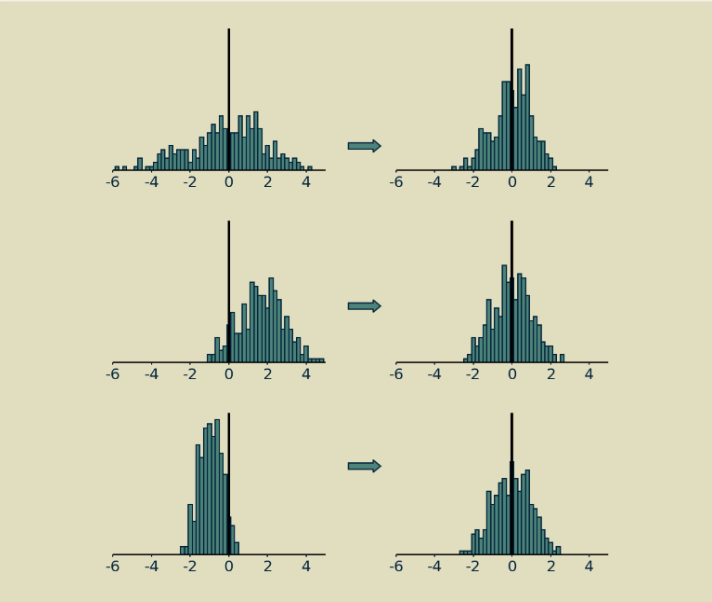
\includegraphics[width=\textwidth]{Layer normalization.png}
\end{figure}

\subsection{Residual Layer(skip connection)}

\[
	x+f(x)
\]
Ngoài việc giúp Gradient Flow tốt hơn, cải thiện việc training, nó còn giúp bổ xung thêm thông tin vị trí khi trước đó qua nhiề lớp đã bị mất dần từ layer thấp lên layer cao hơn.



\subsection{Feed Forward}

$$
	FFN(x,W_1,W_2, b_1,b_2) = max(0,xW_1+b_1)W_2+b_2
$$

\section{Transformer Decoder}

\subsection{Decoder Training}

$\bullet$ Truyền câu mục tiêu vào Decoder để tìm ra câu dự đoán.

$\bullet$ So sánh trực tiếp câu dự đoán với nhãn(Teacher Forcing) để tìm ra giá trị mất mát.

\begin{center}
	\begin{tikzpicture}[
			mynode/.style={draw, text width=0.5cm, align=center, minimum height=0.75cm,line width = 0.5mm}
		]
		\node[mynode] at (0,1) {};
		\node[mynode] at (0,1.75) {};
		\node[mynode] at (0,2.5) {};
		\node[mynode] at (0,3.25) {};

		\draw[->, line width = 0.5mm] (0,4) -- (0,4.75);
		\draw[->, line width = 0.5mm] (0,8.5) -- (0,9.25);
		\node at (0,0) {\textbf{<Start>}};
		\node at (0,9.75) {\textbf{She}};
		\draw[<->, line width = 0.5mm,color = red] (0,10) -- (0,10.5);
		\node at (0,10.75) {\textbf{I}};

		\node[mynode] at (2,1) {};
		\node[mynode] at (2,1.75) {};
		\node[mynode] at (2,2.5) {};
		\node[mynode] at (2,3.25) {};

		\draw[->, line width = 0.5mm] (2,4) -- (2,4.75);
		\draw[->, line width = 0.5mm] (2,8.5) -- (2,9.25);
		\node at (2,0) {\textbf{I}};
		\node at (2,9.75) {\textbf{Went}};
		\draw[<->, line width = 0.5mm,color = red] (2,10) -- (2,10.5);
		\node at (2,10.75) {\textbf{go}};

		\node[mynode] at (4,1) {};
		\node[mynode] at (4,1.75) {};
		\node[mynode] at (4,2.5) {};
		\node[mynode] at (4,3.25) {};

		\draw[->, line width = 0.5mm] (4,4) -- (4,4.75);
		\draw[->, line width = 0.5mm] (4,8.5) -- (4,9.25);
		\node at (4,0) {\textbf{go}};
		\node at (4,9.75) {\textbf{to}};
		\draw[<->, line width = 0.5mm,color = red] (4,10) -- (4,10.5);
		\node at (4,10.75) {\textbf{to}};

		\node[mynode] at (6,1) {};
		\node[mynode] at (6,1.75) {};
		\node[mynode] at (6,2.5) {};
		\node[mynode] at (6,3.25) {};

		\draw[->, line width = 0.5mm] (6,4) -- (6,4.75);
		\draw[->, line width = 0.5mm] (6,8.5) -- (6,9.25);
		\node at (6,0) {\textbf{to}};
		\node at (6,9.75) {\textbf{club}};
		\draw[<->, line width = 0.5mm,color = red] (6,10) -- (6,10.5);
		\node at (6,10.75) {\textbf{school}};

		\node[mynode] at (8,1) {};
		\node[mynode] at (8,1.75) {};
		\node[mynode] at (8,2.5) {};
		\node[mynode] at (8,3.25) {};

		\draw[->, line width = 0.5mm] (8,4) -- (8,4.75);
		\draw[->, line width = 0.5mm] (8,8.5) -- (8,9.25);
		\node at (8,0) {\textbf{school}};
		\node at (8,9.75) {\textbf{<End>}};
		\draw[<->, line width = 0.5mm,color = red] (8,10) -- (8,10.5);
		\node at (8,10.75) {\textbf{<End>}};

		\node[align = center,draw, rounded corners=2mm, minimum width=10cm, minimum height=3cm,line width = 0.5mm, fill = gray!50] at (4,6.5) {\color{red}\textbf{Decoder}};


		\node at (-2,10.75) {\color{blue}\textbf{Label}};
		\node at (-2,9.75) {\color{blue}\textbf{Predicted}};

		\node at (9.65,10.25) {\color{red}\textbf{Loss}};


	\end{tikzpicture}
\end{center}




\subsection{Decoder Inference}

$\bullet$ Truyền từng từ vào để dự đoán từ tiếp theo. Nối từ tiếp theo và dự đoán tiếp tục như thế.Quá trình kết thúc khi gặp token <End> hoặc đạt tới max\_len.
\newpage
\begin{center}
	\begin{tikzpicture}[
			mynode/.style={draw, text width=0.5cm, align=center, minimum height=0.75cm,line width = 0.5mm}
		]
		\node[mynode] at (0,1) {};
		\node[mynode] at (0,1.75) {};
		\node[mynode] at (0,2.5) {};
		\node[mynode] at (0,3.25) {};

		\draw[->, line width = 0.5mm] (0,4) -- (0,4.75);
		\draw[->, line width = 0.5mm] (0,8.5) -- (0,9.25);
		\node at (0,0) {\textbf{<Start>}};
		\node at (0,9.75) {\textbf{She}};
		\draw[->, line width = 0.5mm, color = red] (0,9.25) -- (2,0.25);

		\node[mynode, fill = gray!10] at (2,1) {};
		\node[mynode,fill = gray!10] at (2,1.75) {};
		\node[mynode,fill = gray!10] at (2,2.5) {};
		\node[mynode] at (2,3.25) {};

		\draw[->, line width = 0.5mm] (2,4) -- (2,4.75);
		\draw[->, line width = 0.5mm] (2,8.5) -- (2,9.25);
		\node at (2,0) {\textbf{She}};
		\node at (2,9.75) {\textbf{went}};
		\draw[->, line width = 0.5mm, color = red] (2,9.25) -- (4,0.25);


		\node[mynode,fill = gray!10] at (4,1) {};
		\node[mynode,fill = gray!10] at (4,1.75) {};
		\node[mynode,fill = gray!10] at (4,2.5) {};
		\node[mynode,fill = gray!10] at (4,3.25) {};

		\draw[->, line width = 0.5mm] (4,4) -- (4,4.75);
		\draw[->, line width = 0.5mm] (4,8.5) -- (4,9.25);
		\node at (4,0) {\textbf{went}};
		\node at (4,9.75) {\textbf{to}};
		\draw[->, line width = 0.5mm, color = red] (4,9.25) -- (6,0.25);

		\node[mynode,,fill = gray!10] at (6,1) {};
		\node[mynode,,fill = gray!10] at (6,1.75) {};
		\node[mynode,,fill = gray!10] at (6,2.5) {};
		\node[mynode,,fill = gray!10] at (6,3.25) {};

		\draw[->, line width = 0.5mm] (6,4) -- (6,4.75);
		\draw[->, line width = 0.5mm] (6,8.5) -- (6,9.25);
		\node at (6,0) {\textbf{to}};
		\node at (6,9.75) {\textbf{club}};
		\draw[->, line width = 0.5mm, color = red] (6,9.25) -- (8,0.25);

		\node[mynode,fill = gray!10] at (8,1) {};
		\node[mynode,fill = gray!10] at (8,1.75) {};
		\node[mynode,fill = gray!10] at (8,2.5) {};
		\node[mynode,fill = gray!10] at (8,3.25) {};

		\draw[->, line width = 0.5mm] (8,4) -- (8,4.75);
		\draw[->, line width = 0.5mm] (8,8.5) -- (8,9.25);
		\node at (8,0) {\textbf{club}};
		\node at (8,9.75) {\textbf{<End>}};


		\node[align = center,draw, rounded corners=2mm, minimum width=10cm, minimum height=3cm,line width = 0.5mm, fill = gray!50] at (4,6.5) {\color{red}\textbf{Decoder}};

	\end{tikzpicture}
\end{center}

\subsection{Look Ahead Mask}
$\bullet$ Casual Attention: Cho phép từ kết nối với các từ đã có trước đó và không thể kết nối với các từ phái sau.

\begin{center}
	\begin{tikzpicture}
		\node[draw, rounded corners=2mm, minimum width=3cm, minimum height=1cm,line width = 0.5mm] at (0,0) {\textbf{Matmul}};
		\node[draw, rounded corners=2mm, minimum width=3cm, minimum height=1cm,line width = 0.5mm] at (0,2) {\textbf{Scaled}};
		\node[draw, rounded corners=2mm, minimum width=3cm, minimum height=1cm,line width = 0.5mm, fill = gray!50] at (0,4) {\textbf{Mask(opt.)}};
		\node[draw, rounded corners=2mm, minimum width=3cm, minimum height=1cm,line width = 0.5mm] at (0,6) {\textbf{Softmax}};

		\node[draw, rounded corners=2mm, minimum width=5cm, minimum height=1cm,line width = 0.5mm] at (1,8) {\textbf{Matmul}};

		\draw[->,line width = 0.5mm, color = red] (-0.5,-1.5) --(-0.5,-0.5);
		\draw[->,line width = 0.5mm, color = red] (0.5,-1.5) --(0.5,-0.5);

		\draw[->,line width = 0.5mm, color = red] (0,0.5) --(0,1.5);
		\draw[->,line width = 0.5mm, color = red] (0,2.5) --(0,3.5);
		\draw[->,line width = 0.5mm, color = red] (0,4.5) --(0,5.5);
		\draw[->,line width = 0.5mm, color = red] (0,6.5) --(0,7.5);

		\draw[->,line width = 0.5mm, color = red] (2.5,-1.5) --(2.5,7.5);

		\node at (-0.5,-2) {\large\color{red} \textbf{Q}};
		\node at (0.5,-2) {\large\color{red} \textbf{K}};
		\node at (2.5,-2) {\large\color{red} \textbf{V}};
	\end{tikzpicture}
\end{center}

\begin{center}
	\begin{tikzpicture}[
			mynode/.style={draw, text width=0.8cm, align=center, minimum height=0.75cm,line width = 0.5mm}
		]

		\node[mynode] at (0,1.75) {
			\tiny \textbf{học}};
		\node[mynode] at (0,2.5) {\tiny \textbf{đang}};
		\node[mynode] at (0,3.25) {\tiny \textbf{Tôi}};
		\node[mynode] at (0,4) {\tiny \textbf{<S>}};
		\node[mynode] at (0,4.75) {};

		\node[mynode] at (1.08,1.75) {6};
		\node[mynode] at (1.08,2.5) {3};
		\node[mynode] at (1.08,3.25) {2};
		\node[mynode] at (1.08,4) {1};
		\node[mynode] at (1.08,4.75) {\tiny \textbf{<S>}};

		\node[mynode] at (2.16,1.75) {8};
		\node[mynode] at (2.16,2.5) {7};
		\node[mynode] at (2.16,3.25) {6};
		\node[mynode] at (2.16,4) {5};
		\node[mynode] at (2.16,4.75) {\tiny \textbf{Tôi}};

		\node[mynode] at (3.24,1.75) {8};
		\node[mynode] at (3.24,2.5) {11};
		\node[mynode] at (3.24,3.25) {10};
		\node[mynode] at (3.24,4) {9};
		\node[mynode] at (3.24,4.75) {\tiny \textbf{đang}};

		\node[mynode] at (4.32,1.75) {9};
		\node[mynode] at (4.32,2.5) {15};
		\node[mynode] at (4.32,3.25) {6};
		\node[mynode] at (4.32,4) {13};
		\node[mynode] at (4.32,4.75) {\tiny \textbf{học}};


		\node[mynode] at (9,1.75) {
			\tiny \textbf{học}};
		\node[mynode] at (9,2.5) {\tiny \textbf{đang}};
		\node[mynode] at (9,3.25) {\tiny \textbf{Tôi}};
		\node[mynode] at (9,4) {\tiny \textbf{<S>}};
		\node[mynode] at (9,4.75) {};

		\node[mynode] at (10.08,1.75) {6};
		\node[mynode] at (10.08,2.5) {3};
		\node[mynode] at (10.08,3.25) {2};
		\node[mynode] at (10.08,4) {1};
		\node[mynode] at (10.08,4.75) {\tiny \textbf{<S>}};

		\node[mynode] at (11.16,1.75) {8};
		\node[mynode] at (11.16,2.5) {7};
		\node[mynode] at (11.16,3.25) {6};
		\node[mynode] at (11.16,4) {\color{red}-inf};
		\node[mynode] at (11.16,4.75) {\tiny \textbf{tôi}};

		\node[mynode] at (12.24,1.75) {8};
		\node[mynode] at (12.24,2.5) {11};
		\node[mynode] at (12.24,3.25) {\color{red}-inf};
		\node[mynode] at (12.24,4) {\color{red}-inf};
		\node[mynode] at (12.24,4.75) {\tiny \textbf{đang}};

		\node[mynode] at (13.32,1.75) {9};
		\node[mynode] at (13.32,2.5) {\color{red}-inf};
		\node[mynode] at (13.32,3.25) {\color{red}-inf};
		\node[mynode] at (13.32,4) {\color{red}-inf};
		\node[mynode] at (13.32,4.75) {\tiny \textbf{học}};

		\draw[->, line width = 0.5mm, color = red] (5,3.25) -- (8.25,3.25);
		\node at (6.5,3.5) {\color{red}\textbf{Look Ahead}};
		\node at (6.5,3) {\color{red}\textbf{Mask}};

		\node[mynode] at (9,-6) {
			\tiny \textbf{học}};
		\node[mynode] at (9,-5.25) {\tiny \textbf{đang}};
		\node[mynode] at (9,-4.5) {\tiny \textbf{Tôi}};
		\node[mynode] at (9,-3.75) {\tiny \textbf{<S>}};
		\node[mynode] at (9,-3) {};

		\node[mynode] at (10.08,-6) {\small 0.028};
		\node[mynode] at (10.08,-5.25) {\small 0.001};
		\node[mynode] at (10.08,-4.5) {\small 0.018};
		\node[mynode] at (10.08,-3.75) {1};
		\node[mynode] at (10.08,-3) {\tiny \textbf{<S>}};

		\node[mynode] at (11.16,-6) {\small 0.206};
		\node[mynode] at (11.16,-5.25) {\small 0.063};
		\node[mynode] at (11.16,-4.5) {\small 0.982};
		\node[mynode] at (11.16,-3.75) {0};
		\node[mynode] at (11.16,-3) {\tiny \textbf{tôi}};

		\node[mynode] at (12.24,-6) {\small 0.206};
		\node[mynode] at (12.24,-5.25) {\small 0.935};
		\node[mynode] at (12.24,-4.5) {0};
		\node[mynode] at (12.24,-3.75) {0};
		\node[mynode] at (12.24,-3) {\tiny \textbf{đang}};

		\node[mynode] at (13.32,-6) {\small 0.560};
		\node[mynode] at (13.32,-5.25) {0};
		\node[mynode] at (13.32,-4.5) {0};
		\node[mynode] at (13.32,-3.75) {0};
		\node[mynode] at (13.32,-3) {\tiny \textbf{học}};

		\draw[->, line width = 0.5mm, color = red] (11.16,1.25) -- (11.16,-2.5);
		\node at (12.25,-0.25) {\color{red}\textbf{Softmax}};

	\end{tikzpicture}
\end{center}

\subsection{GPT}

GPT sử dụng Transformer decoder, là auto-regressive model.

\begin{center}
	\begin{tikzpicture}
		\node[align = center,draw, rounded corners=2mm, minimum width=5cm, minimum height=8cm,line width = 0.5mm, fill = gray!30] at (0,3) {};

		\node[align = center,draw, rounded corners=2mm, minimum width=4cm, minimum height=1cm,line width = 0.5mm, fill = gray!1] at (0,0) {Decoder Block};

		\node[align = center,draw, rounded corners=2mm, minimum width=4cm, minimum height=1cm,line width = 0.5mm, fill = gray!1] at (0,1.5) {Decoder Block};

		\node[align = center,draw, rounded corners=2mm, minimum width=4cm, minimum height=1cm,line width = 0.5mm, fill = gray!1] at (0,6) {Decoder Block};

		\node[align = center,draw, rounded corners=2mm, minimum width=4cm, minimum height=1cm,line width = 0.5mm, fill = gray!10] at (0,4.5) {Decoder Block};

		\node at (0,3) {$\cdots$};

		\draw[line width = 0.5mm] (2,2) -- (4.5,5.75);
		\draw[line width = 0.5mm] (2,1) -- (4.5,-1.2);


		\node[dashed,draw, rounded corners=2mm, minimum width=5cm, minimum height=7.25cm,line width = 0.5mm] at (7,2.3) {};

		\draw[->, line width = 0.5mm ] (7,-1.75) -- (7,-0.8);
		\draw[->, line width = 0.5mm ] (7,0) -- (7,1.25);

		\draw[->, line width = 0.5mm ] (7,4) -- (7,5);
		\draw[->, line width = 0.5mm ] (7,1) -- (7,3.05);

		\draw[->, line width = 0.5mm ] (7,4) -- (7,6.5);

		\draw[line width = 0.5mm ] (7,-1.15) -- (9.3,-1.15);

		\draw[line width = 0.5mm ] (9.3,-1.175) -- (9.3,1.5);

		\draw[->,line width = 0.5mm ] (9.325,1.5) -- (8.75,1.5);

		\draw[line width = 0.5mm ] (7,2.65) -- (9.3,2.65);

		\draw[line width = 0.5mm ] (9.3,2.625) -- (9.3,5);

		\draw[->,line width = 0.5mm ] (9.325,5) -- (8.75,5);

		\node[align = center, draw, rounded corners=1.5mm, minimum width=3.5cm, minimum height=1.25cm, fill = orange!30,line width = 0.5mm] at (7,0) {\small \color{black}Masked\\\small \color{black}Multi - headed\\ \small \color{black}Attention};

		\node[draw, rounded corners=1.5mm, minimum width=3.5cm, minimum height=0.75cm, fill = yellow!30,line width = 0.5mm] at (7,1.5) {\small \color{black}Add \& Norm};

		\node[draw, rounded corners=1.5mm, minimum width=3.5cm, minimum height=0.75cm, fill = yellow!30, line width = 0.5mm] at (7,5) {\small \color{black}Add \& Norm};

		\node[align = center, draw, rounded corners=1.5mm, minimum width=3.5cm, minimum height=1.25cm, fill = blue!30,line width = 0.5mm] at (7,3.7) {\small \color{black}Feed\\ \small \color{black}Forward};

	\end{tikzpicture}
\end{center}
\chapter{BERT(Bidirectional Encoder Representations from Transformers)}

$\bullet$ BERT được xây dựng là một pre-trained học từ dữ liệu không nhãn. BERT được pre-trained từ hai bài toán:

$\hspace*{0.5cm} \circ$ Dự đoán từ còn thiếu( Masked Sentence)

$\hspace*{0.5cm} \circ$ Hai câu có hay đi liền với nhau không.

$\bullet$ Từ pre-trained này có thể sử dụng để finetune trên dữ liệu có nhãn.

$\hspace*{0.5cm} \circ$ NER - Nhận diện thực thể trong câu

$\hspace*{0.5cm} \circ$ SQuAD - trả lời đáp án trong văn bản( token start - end)

$\hspace*{0.5cm} \circ$ MNLI - Xác định mối quan hệ của hai câu ( có đi liền nhau không, tương phản, bổ trợ, ...)

\begin{figure*}[h]
	\begin{center}
		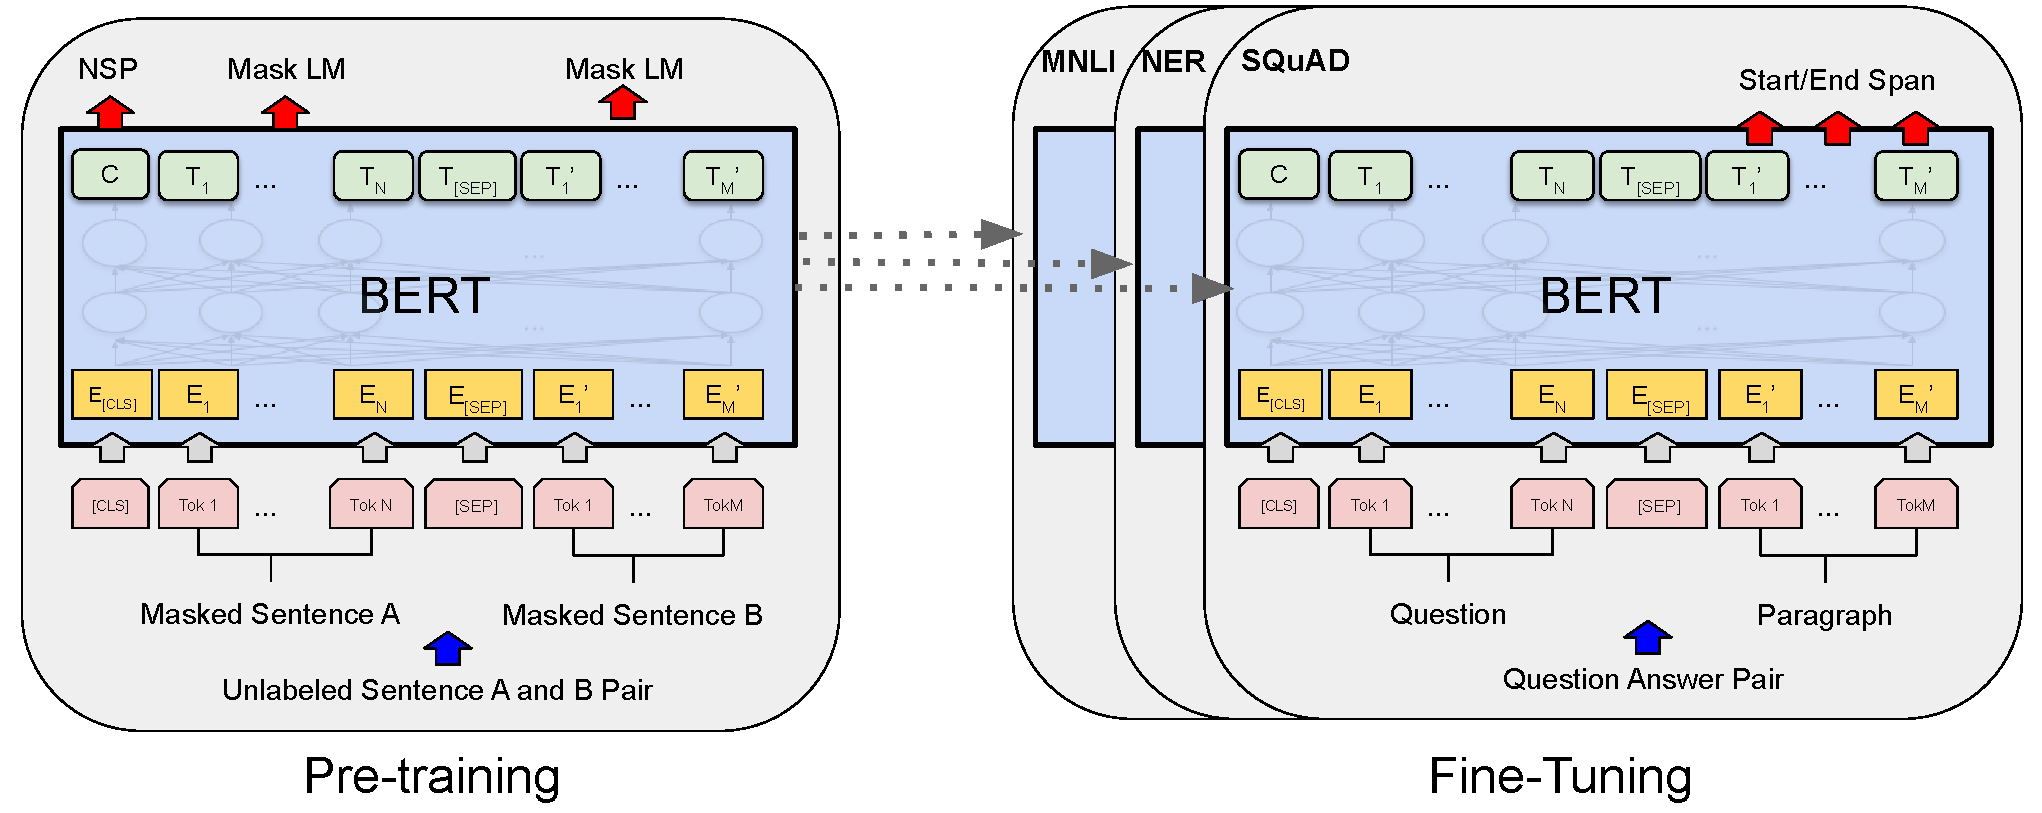
\includegraphics[width=1\textwidth]{BERT_Overall.pdf}
	\end{center}
\end{figure*}

\newpage

$\bullet$ Quy trình pre-training BERT:

$\hspace*{0.5cm} \circ$ \textbf{Nhiệm vụ 1: Masked Language Model}

\begin{center}
	\begin{tikzpicture}[
			mynode/.style={draw, text width=0.8cm, align=center, minimum height=0.75cm,line width = 0.5mm}
		]

		\node[align = center,draw, rounded corners=2mm, minimum width=10cm, minimum height=3cm,line width = 0.5mm, fill = blue!30] at (0,2) {\textbf{BERT} \\ \textbf{Transformer Encoder}};

		\draw[->, line width = 0.5mm] (-4,-1.5) --(-4,0);
		\draw[->, line width = 0.5mm] (-2,-1.5) --(-2,0);
		\draw[->, line width = 0.5mm] (0,-1.5) --(0,0);
		\draw[->, line width = 0.5mm] (2,-1.5) --(2,0);
		\draw[->, line width = 0.5mm] (4,-1.5) --(4,0);

		\node at (-4,-2) {\textbf{[CLS]}};
		\node at (-2,-2) {\textbf{I}};
		\node at (0,-2) {\textbf{am}};
		\node at (2,-2) {\textbf{[Mark]}};
		\node at (4,-2) {\textbf{math}};

		\draw[->, line width = 0.5mm] (-4,4) --(-4,5.5);
		\draw[->, line width = 0.5mm] (-2,4) --(-2,5.5);
		\draw[->, line width = 0.5mm] (0,4) --(0,5.5);
		\draw[->, line width = 0.5mm] (2,4) --(2,7);
		\draw[->, line width = 0.5mm] (4,4) --(4,5.5);

		\node at (2,7.5) {\textbf{FFNN+Softmax}};

		\draw[->, line width = 0.5mm] (2,8) --(2,9.5);

		\node[mynode] at (-0.3,10) {\small \textbf{0.1}};
		\node[mynode] at (0.8,10) {\small \textbf{0.05}};
		\node[mynode] at (1.9,10) {\small \textbf{0.1}};
		\node[mynode] at (3,10) {\small \textbf{0.5}};
		\node[mynode] at (4.1,10) {\small \textbf{0.25}};


	\end{tikzpicture}
\end{center}

$\hspace*{1cm}$- Để train mô hình này, việc ngẫu nhiên che đi (mask) một lượng \% tokens trong văn bản sau đó huấn luyện lượng tokens còn lại để dự đoán ra tokens bị che này.

$\hspace*{1cm}$- Cụ thể  che đi 15\% số lượng WordPiece Tokens ở mỗi chuỗi đầu vào một cách ngẫu nhiên.

$\hspace*{1cm}$- Trong 15\% này:

$\hspace*{1.5cm}$+ thay thế 80\% bằng token [MASK]

$\hspace*{1.5cm}$+ thay thế 10\% bằng token ngẫu nhiên

$\hspace*{1.5cm}$+ giữ nguyên 10\% còn lại.

$\hspace*{1cm}$- Cách làm này là do token [MASK] chỉ Sat hiện khi \textbf{train pre-trained} và không xuất hiện khi chúng ta \textbf{fine-tune}.

\newpage

$\hspace*{0.5cm} \circ$ \textbf{Nhiệm vụ 2: Dự đoán câu tiếp theo}

\begin{center}
	\begin{tikzpicture}[
			mynode/.style={draw, text width=0.8cm, align=center, minimum height=0.75cm,line width = 0.5mm}
		]

		\node[align = center,draw, rounded corners=2mm, minimum width=15cm, minimum height=3cm,line width = 0.5mm, fill = blue!30] at (0,1.75) {\textbf{BERT} \\ \textbf{Transformer Encoder}};

		\draw[->, line width = 0.5mm] (-7,-1.5) --(-7,0);
		\draw[->, line width = 0.5mm] (-5.5,-1.5) --(-5.5,0);
		\draw[->, line width = 0.5mm] (-4,-1.5) --(-4,0);
		\draw[->, line width = 0.5mm] (-2.5,-1.5) --(-2.5,0);
		\draw[->, line width = 0.5mm] (-1,-1.5) --(-1,0);
		\draw[->, line width = 0.5mm] (0.5,-1.5) --(0.5,0);
		\draw[->, line width = 0.5mm] (2,-1.5) --(2,0);
		\draw[->, line width = 0.5mm] (3.5,-1.5) --(3.5,0);
		\draw[->, line width = 0.5mm] (5,-1.5) --(5,0);
		\draw[->, line width = 0.5mm] (6.5,-1.5) --(6.5,0);

		\node at (-7,-2) {\textbf{[CLS]}};
		\node at (-5.5,-2) {\textbf{}};
		\node at (-4,-2) {\textbf{[MASK]}};
		\node at (-2.5,-2) {\textbf{}};
		\node at (-1,-2) {\textbf{[SEP]}};
		\node at (0.5,-2) {\textbf{}};
		\node at (2,-2) {\textbf{}};
		\node at (3.5,-2) {\textbf{}};
		\node at (5,-2) {\textbf{[MASK]}};
		\node at (6.5,-2) {\textbf{[SEP]}};


		\draw[->, line width = 0.5mm] (-7,4) --(-7,7);
		\draw[->, line width = 0.5mm] (-5.5,4) --(-5.5,5.5);
		\draw[->, line width = 0.5mm] (-4,4) --(-4,5.5);
		\draw[->, line width = 0.5mm] (-2.5,4) --(-2.5,5.5);
		\draw[->, line width = 0.5mm] (-1,4) --(-1,5.5);
		\draw[->, line width = 0.5mm] (0.5,4) --(0.5,5.5);
		\draw[->, line width = 0.5mm] (2,4) --(2,5.5);
		\draw[->, line width = 0.5mm] (3.5,4) --(3.5,5.5);
		\draw[->, line width = 0.5mm] (5,4) --(5,5.5);
		\draw[->, line width = 0.5mm] (6.5,4) --(6.5,5.5);

		\node at (-7,7.5) {\textbf{FFNN+Softmax}};

		\draw[->, line width = 0.5mm] (-7,8) --(-7,9.5);

		\node[mynode] at (-7.5,10) {\small \textbf{0.1}};
		\node[mynode] at (-6.4,10) {\small \textbf{0.9}};

		\node[mynode, text width=1.5cm] at (-7.9,11) {\small \textbf{IsNext}};
		\node[mynode, text width=1.5cm] at (-6.1,11) {\small \textbf{NotNext}};
	\end{tikzpicture}
\end{center}


$\hspace*{1cm}$- Pre-train sẽ được train cho bài toán phân loại hai câu có đi liền với nhau hay không.

$\hspace*{1cm}$- Dữ liệu được train sẽ bao gồm các cặp câu A-B trong đó:

$\hspace*{1.5cm}$+ 50\% câu B đi theo sau câu A với nhãn dự đoán là IsNext

$\hspace*{1.5cm}$+ 50\% câu B ngẫu nhiên từ trong ngữ liệu với nhãn dự đoán là NotNext

$\hspace*{1cm}$- Hai câu này được thêm những Token để trở thành dạng sau:

$\hspace*{5cm}$\textbf{[CLS] A [SEP] B [SEP]}

$\hspace*{1cm}$- Trong đó:

$\hspace*{1.5cm}$+ [CLS] là token sentence-level classification ở đầu. Token này sẽ thực hiện attention với tất cả các từ trong câu. Thực tế token này sau khi đi qua BERT thì vector của nó có thể sử dụng cho bài toán phân loại câu.

$\hspace*{1.5cm}$+ [SEP] là token để chia cắt các chuỗi câu. Ví dụ bài toán dịch máy thì [SEP] chia câu được dịch và câu dịch.

\newpage

$\bullet$ Một số Token đặc biệt: \\

\begin{tabular}{|p{2cm}|p{4cm}|p{8cm}|}
	\hline
	Token              & Type       & Describe                                                                                                                                                                                                                                                                                                                                                                     \\
	\hline
	\color{blue} [CLS] & phân loại  & BERT chèn token này vào đầu mỗi chuỗi đầu vào.n Trong các nhiệm vụ liên quan đến phân loại hoặc biểu diễn toàn bộ chuỗi đầu vào( như phân tích cảm xúc), trạng thái ẩn cuosi cùng tương ứng với token này được sử dụng làm biểu diễn tổng hợp cho các nhiệm vụ phân loại.                                                                                                    \\
	\hline
	\color{blue} [SEP] & Phân tách  & Token "phân tách" được sử dụng trong BERT để phân tách các câu hoặc phân tách các đoạn khác nhau trong cùng một đầu vào. Nó sử dụng cho các nhiệm vụ liên quan đến nhiều đầu vào như trả lời câu hỏi( nơi mà mô hình cần phân biệt giữa câu hỏi và đoạn văn) hoặc các nhiệm vụ cặp câu( như phát hiện cụm từ đồng nghĩa).                                                    \\
	\hline
	\color{blue} [PAD] & Đệm        & Token "đệm" này được sử dụng để lấp đầy các chuỗi để tất cả các đầu vào trong một batch có cùng độ dài. Việc đệm là cần thiết vì kiến trúc Transformer(mà BERT dựa trên) yêu cầu đầu vào phải có cùng kích thước(size).                                                                                                                                                      \\
	\hline
	\color{blue}[MASK] & Che        & Được sử dụng chủ yếu trongt quá trình tiền huấn luyện của BERT trên nhiệm vụ MLM (Mask Language Model) nơi các token ngẫu nhiên trong đầu vào được thay thế bằng token này. BERT sau đó được huấn luyện để dự đoán giá trị gốc của các từ bị chem dựa chỉ vào ngữ cảnh của chúng. Điều này giúp mô hình hiểu ngôn ngữ tốt hơn và cải thiện khả nặng dự đoán các từ bị thiếu. \\
	\hline
	\color{blue}[UNK]  & Không biết & Nó được sử dụng khi một từ không được tìm thấy trong vocal của BERT. Vì BERT sử dụng từ vựng cố định, bất kì từ nào không tìm thấy sẽ thay thế bằng token [UNK]                                                                                                                                                                                                              \\
	\hline
\end{tabular}


\section{Tokenizing and reperesentation}
$\bullet$ Quy trình tiếp theo: Câu sẽ được biểu diễn lại:

$\hspace*{0.5cm} \circ$ Qua Token Embeddings để tách token

$\hspace*{0.5cm} \circ$ Qua Segment Embeddings để cập nhật thông tin thuộc chuỗi nào. Ví dụ token thuộc chuỗi A sẽ được cộng thêm giá trị $E_A $ có thể bằng 0 còn token thuộc chuỗi B sẽ được cộng thêm giá trị $E_B$ có thể bằng 1.

$\hspace*{0.5cm} \circ$ Bổ sung thêm Embdding vị trí cho từng token
\begin{figure*}[ht]
	\begin{center}
		\hspace{-0.2in}
		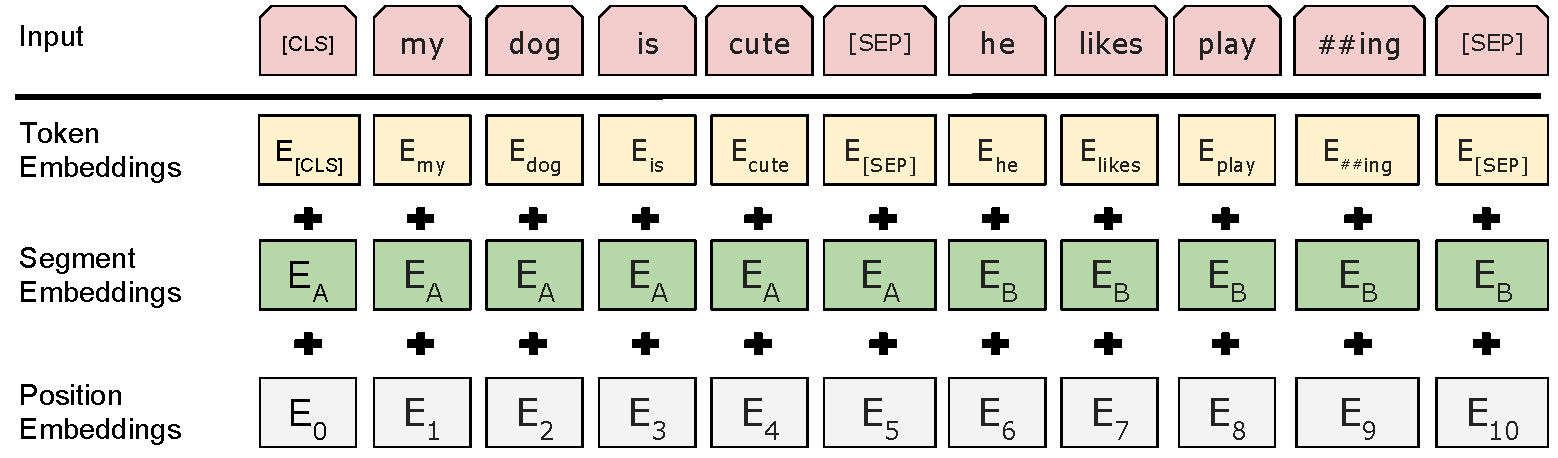
\includegraphics[width=360px]{Input_Emebeddings.pdf}
	\end{center}
\end{figure*}

\section{Fine-tuning BERT on Difference Tasks}

\begin{figure}[h]
	\begin{center}
		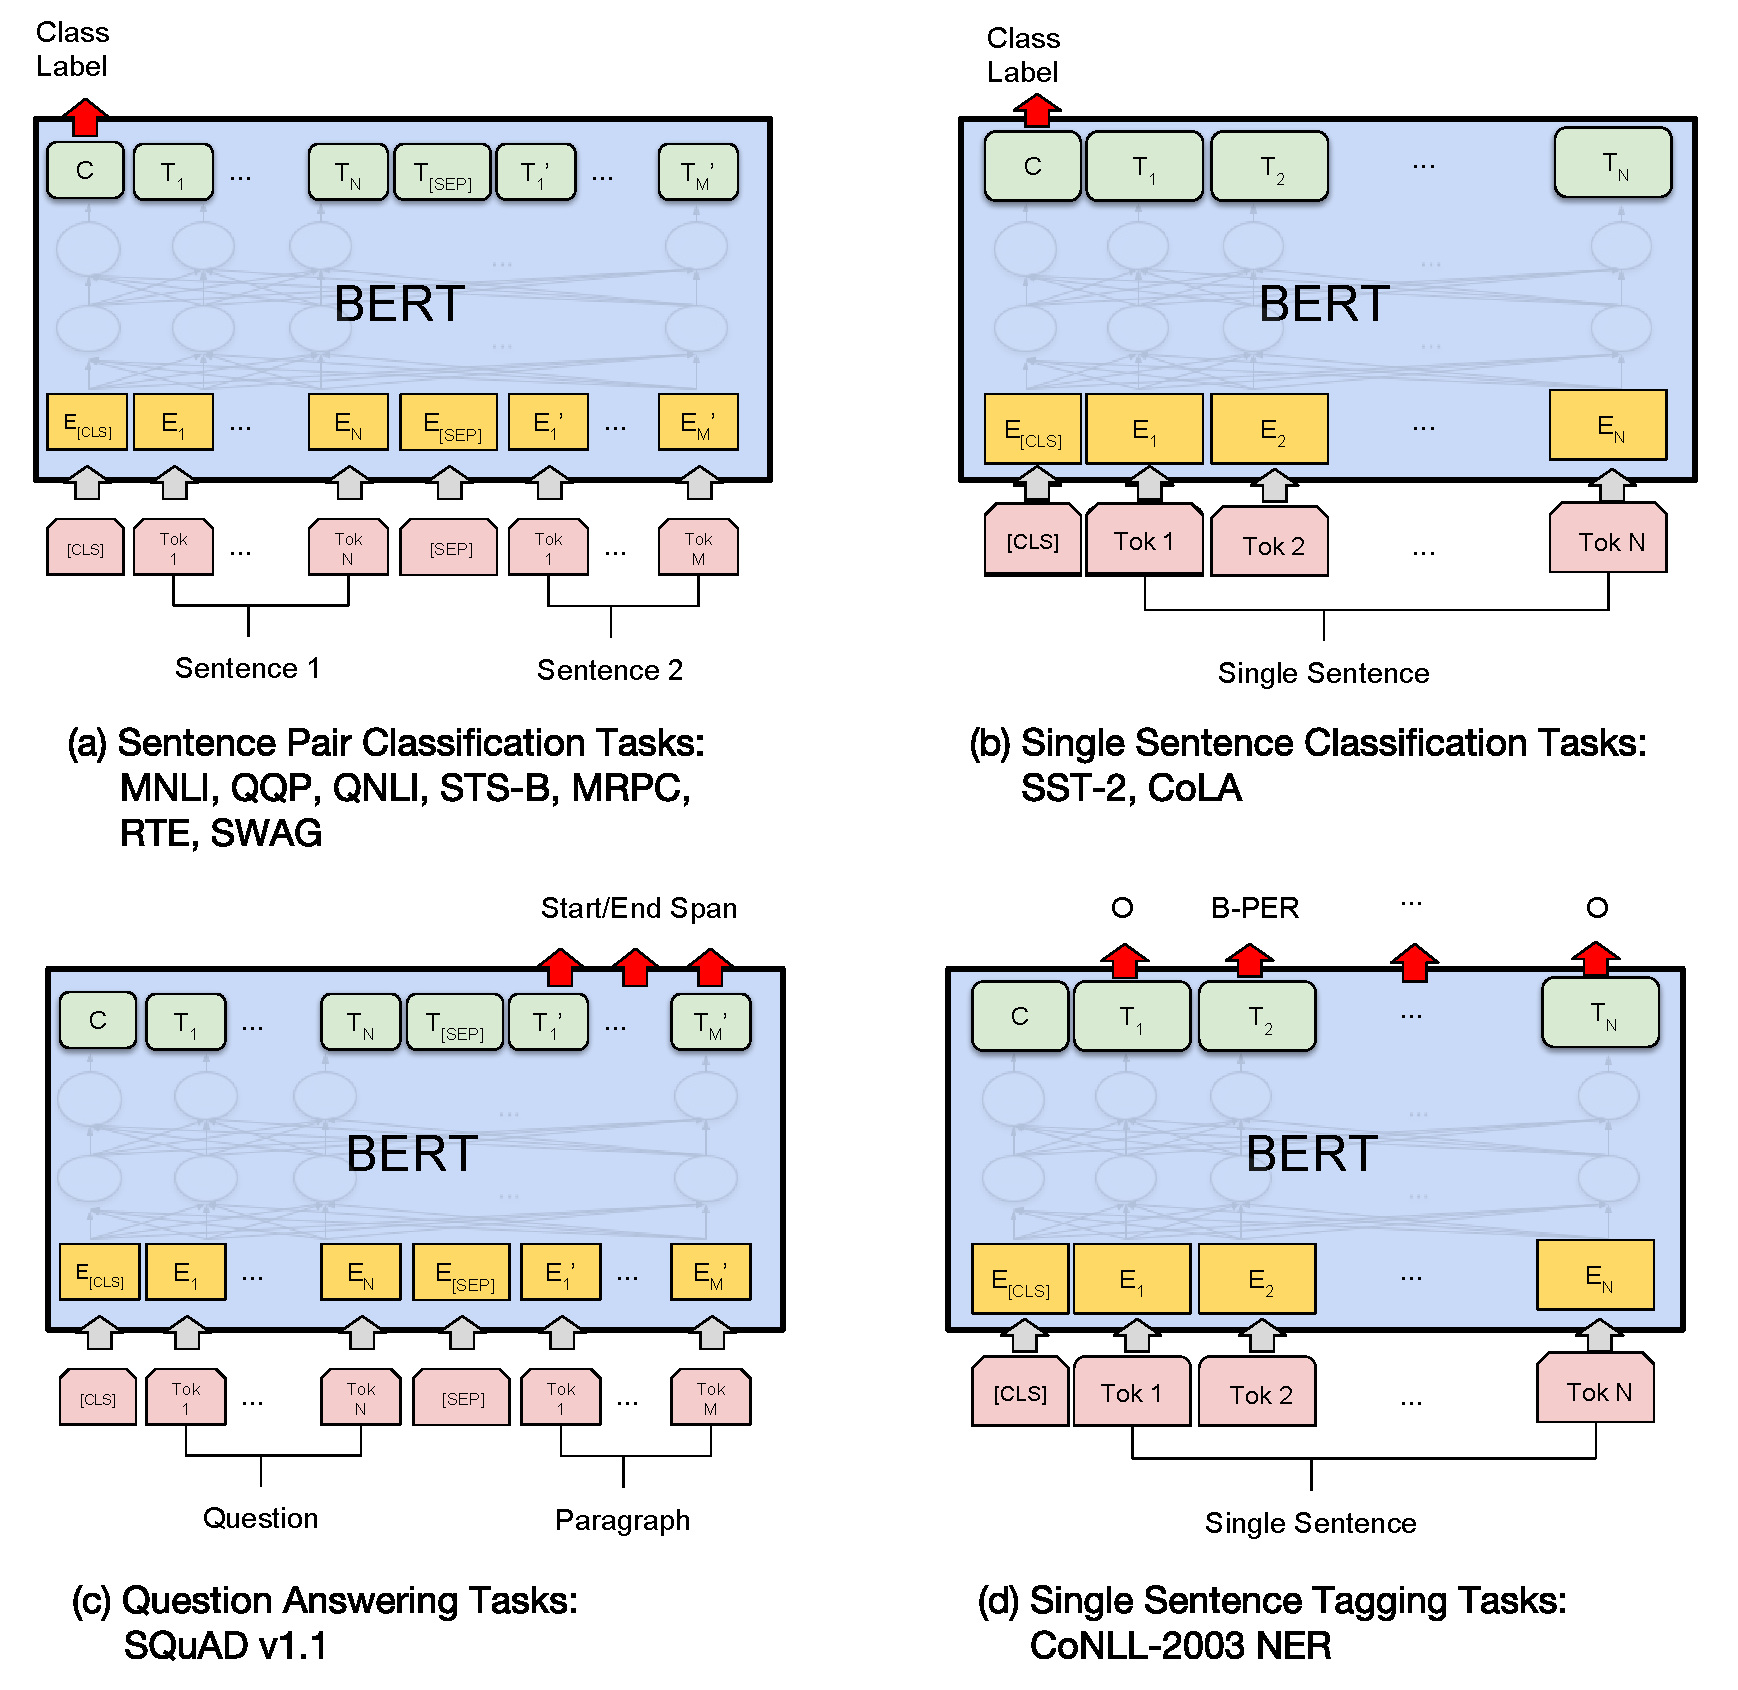
\includegraphics[width=0.85\textwidth]{BERT_fine_tune.pdf}
	\end{center}
\end{figure}

\newpage

\subsection{Fine-tune on the sentence pair problem}


\begin{figure}[h]
	\begin{center}
		% left bottom right top
		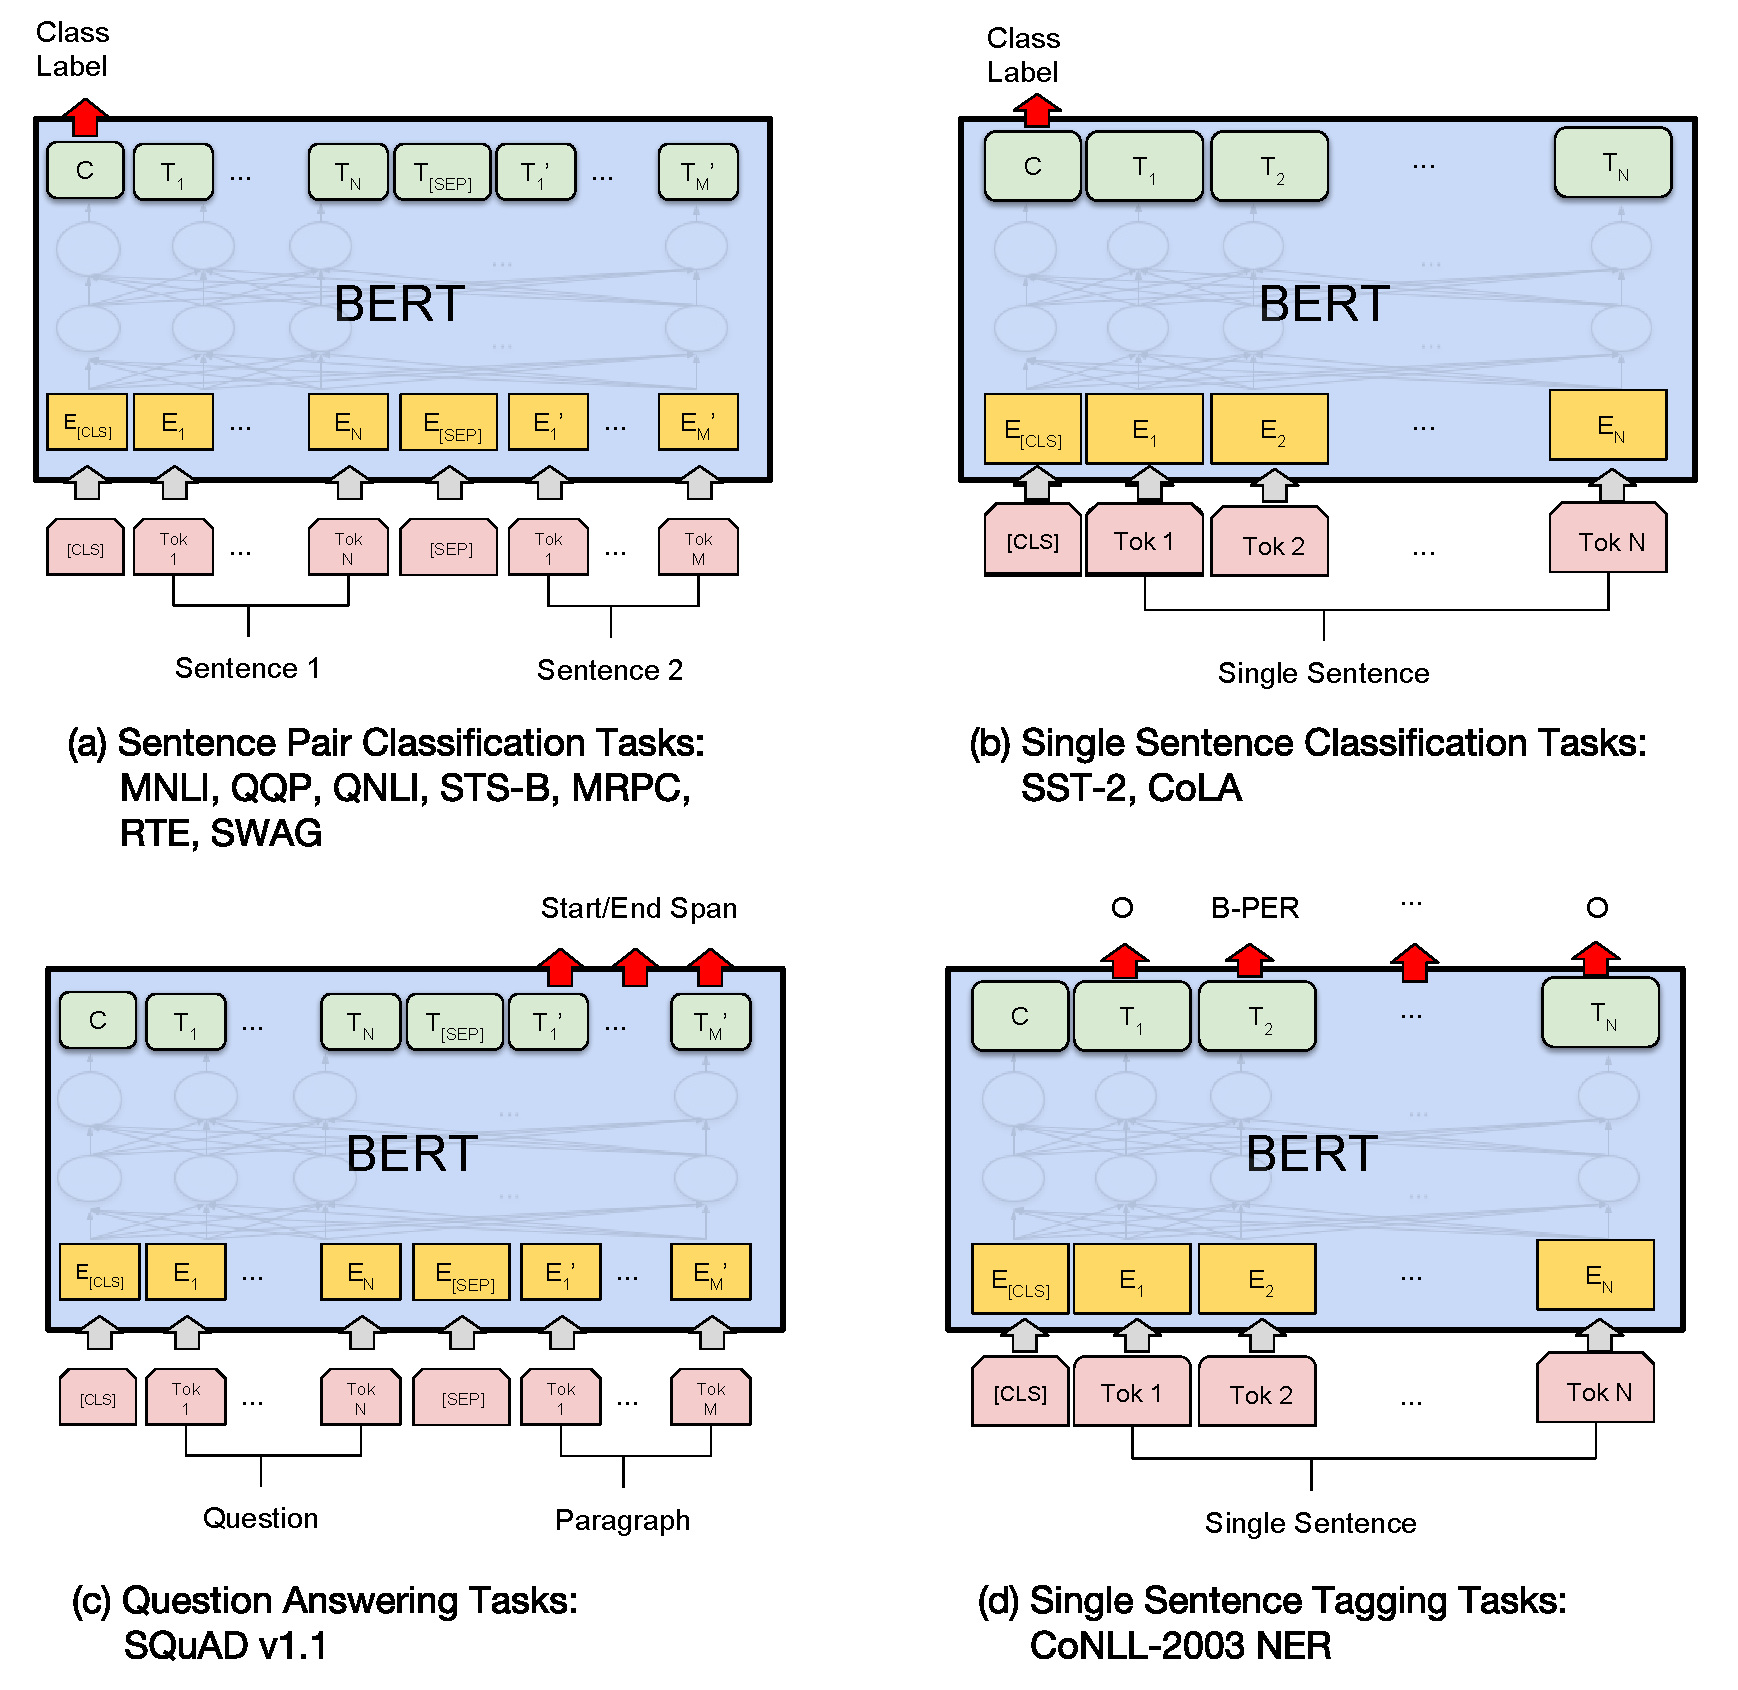
\includegraphics[trim=0 470 440 0, clip,width=1\textwidth]{BERT_fine_tune.pdf}
	\end{center}
\end{figure}

\begin{center}
	\begin{tabular}{|p{2cm}|p{10cm}|}
		\hline
		\color{blue}MNLI  & \color{black}Multi Natural Language Interface           \\
		\hline
		\color{blue}QQP   & \color{black} Quara Question Pairs                      \\
		\hline
		\color{blue}QNLI  & \color{black}Question Natural Language Interface        \\
		\hline
		\color{blue}STS-B & \color{black} The Semantic Textual Similarity Benchmark \\
		\hline
		\color{blue}MRPC  & \color{black} Microsoft Reseach Paraphrase Corpus       \\
		\hline
		\color{blue}RTE   & \color{black} Recognizing Textual Entailment            \\
		\hline
		\color{blue}SWAG  & \color{black} Situations With Adversarial Generation    \\
		\hline
	\end{tabular}
\end{center}

\newpage

\subsection{Fine-Tune on the sentence pair problem}

\begin{figure}[h]
	\begin{center}
		% left bottom right top
		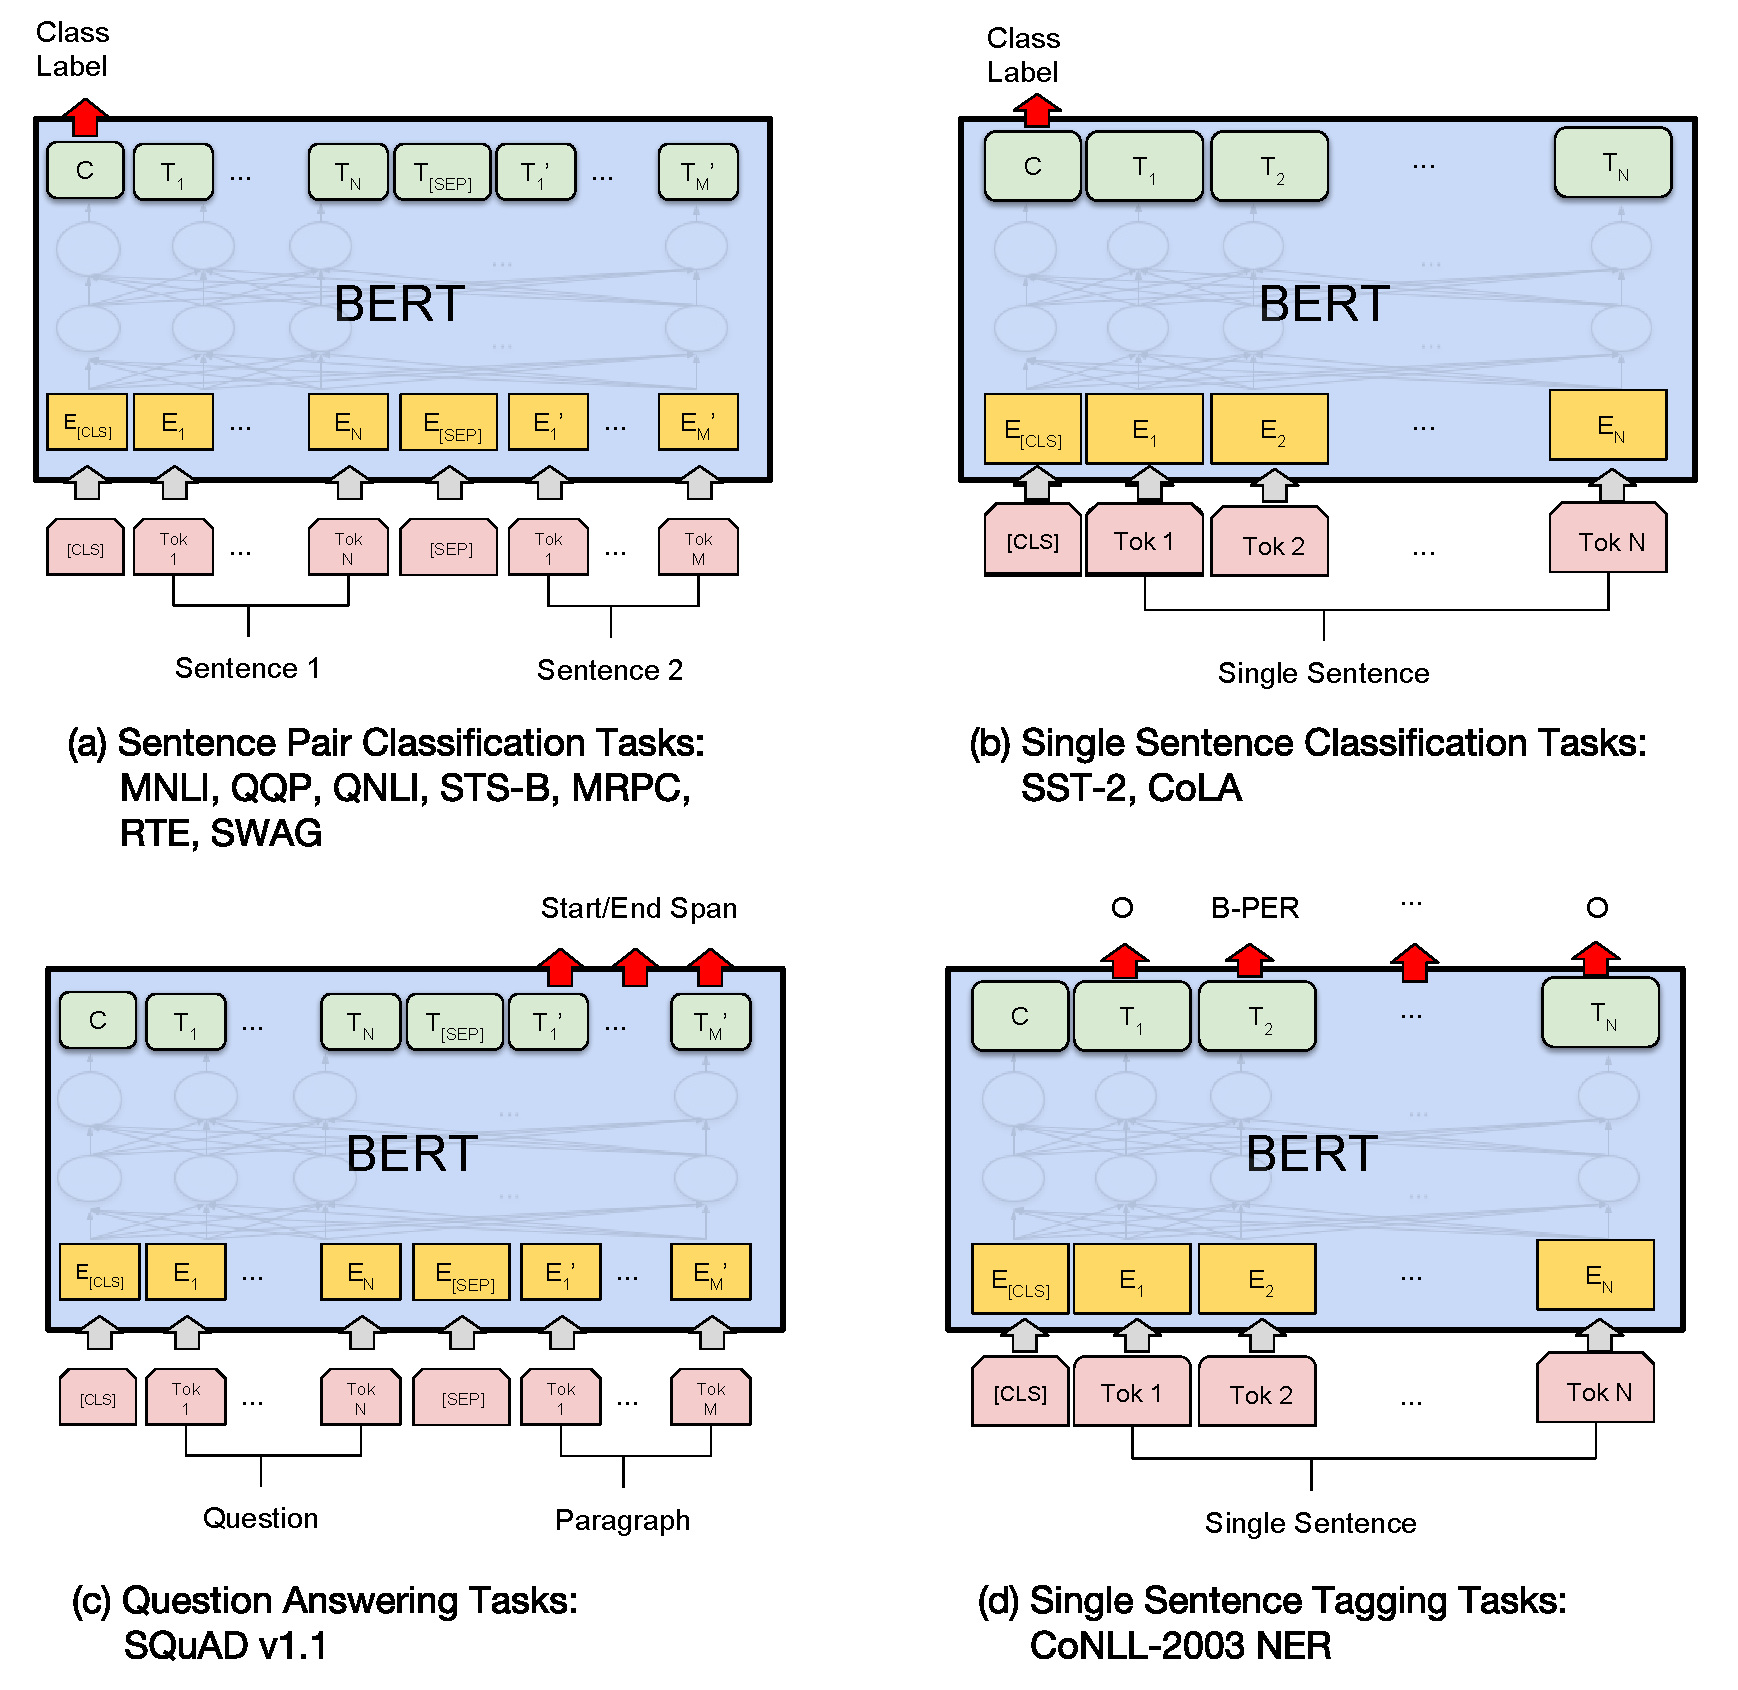
\includegraphics[trim=0 470 440 0, clip,width=1\textwidth]{BERT_fine_tune.pdf}
	\end{center}
\end{figure}

Input  :

\textbf{[CLS] $Token_1$ $Token_2$ $\cdots$ $Token_n$ [SEP] $Token^{'}_{1}$ $Token^{'}_{2}$ $\cdots$ $Token^{'}_{m}$ [SEP]}

Label: 0-5

Explain:

\begin{center}
	\begin{tabular}{|p{6cm}|p{6cm}|p{1.5cm}|}
		\hline
		Sentence 1                                 & sentence 2                                        & Label \\
		\hline
		A plane is taking off                      & An airplane is taking off                         & 5.00  \\
		\hline
		Three men are playing chess                & Two men are playing chess                         & 2.60  \\
		\hline
		Severe Gales As Storm Clodagh Hits Britain & Merkel pledges NATO solidarity with Latvia        & 0.00  \\
		\hline
		A man is playing a large flute             &
		A man is playing a flute                   & 3.80                                                      \\
		\hline
		China, India vow to further bilateral ties & China Scrambles to Reassure Jittery Stock Traders & 0.00  \\
		\hline
		A man is playing the cello                 & A man seated is playing the cello                 & 4.25  \\
		\hline
	\end{tabular}
\end{center}

\newpage

\subsection{Fine-tune on the sentence classification problem}

\begin{figure}[h]
	\begin{center}
		% left bottom right top
		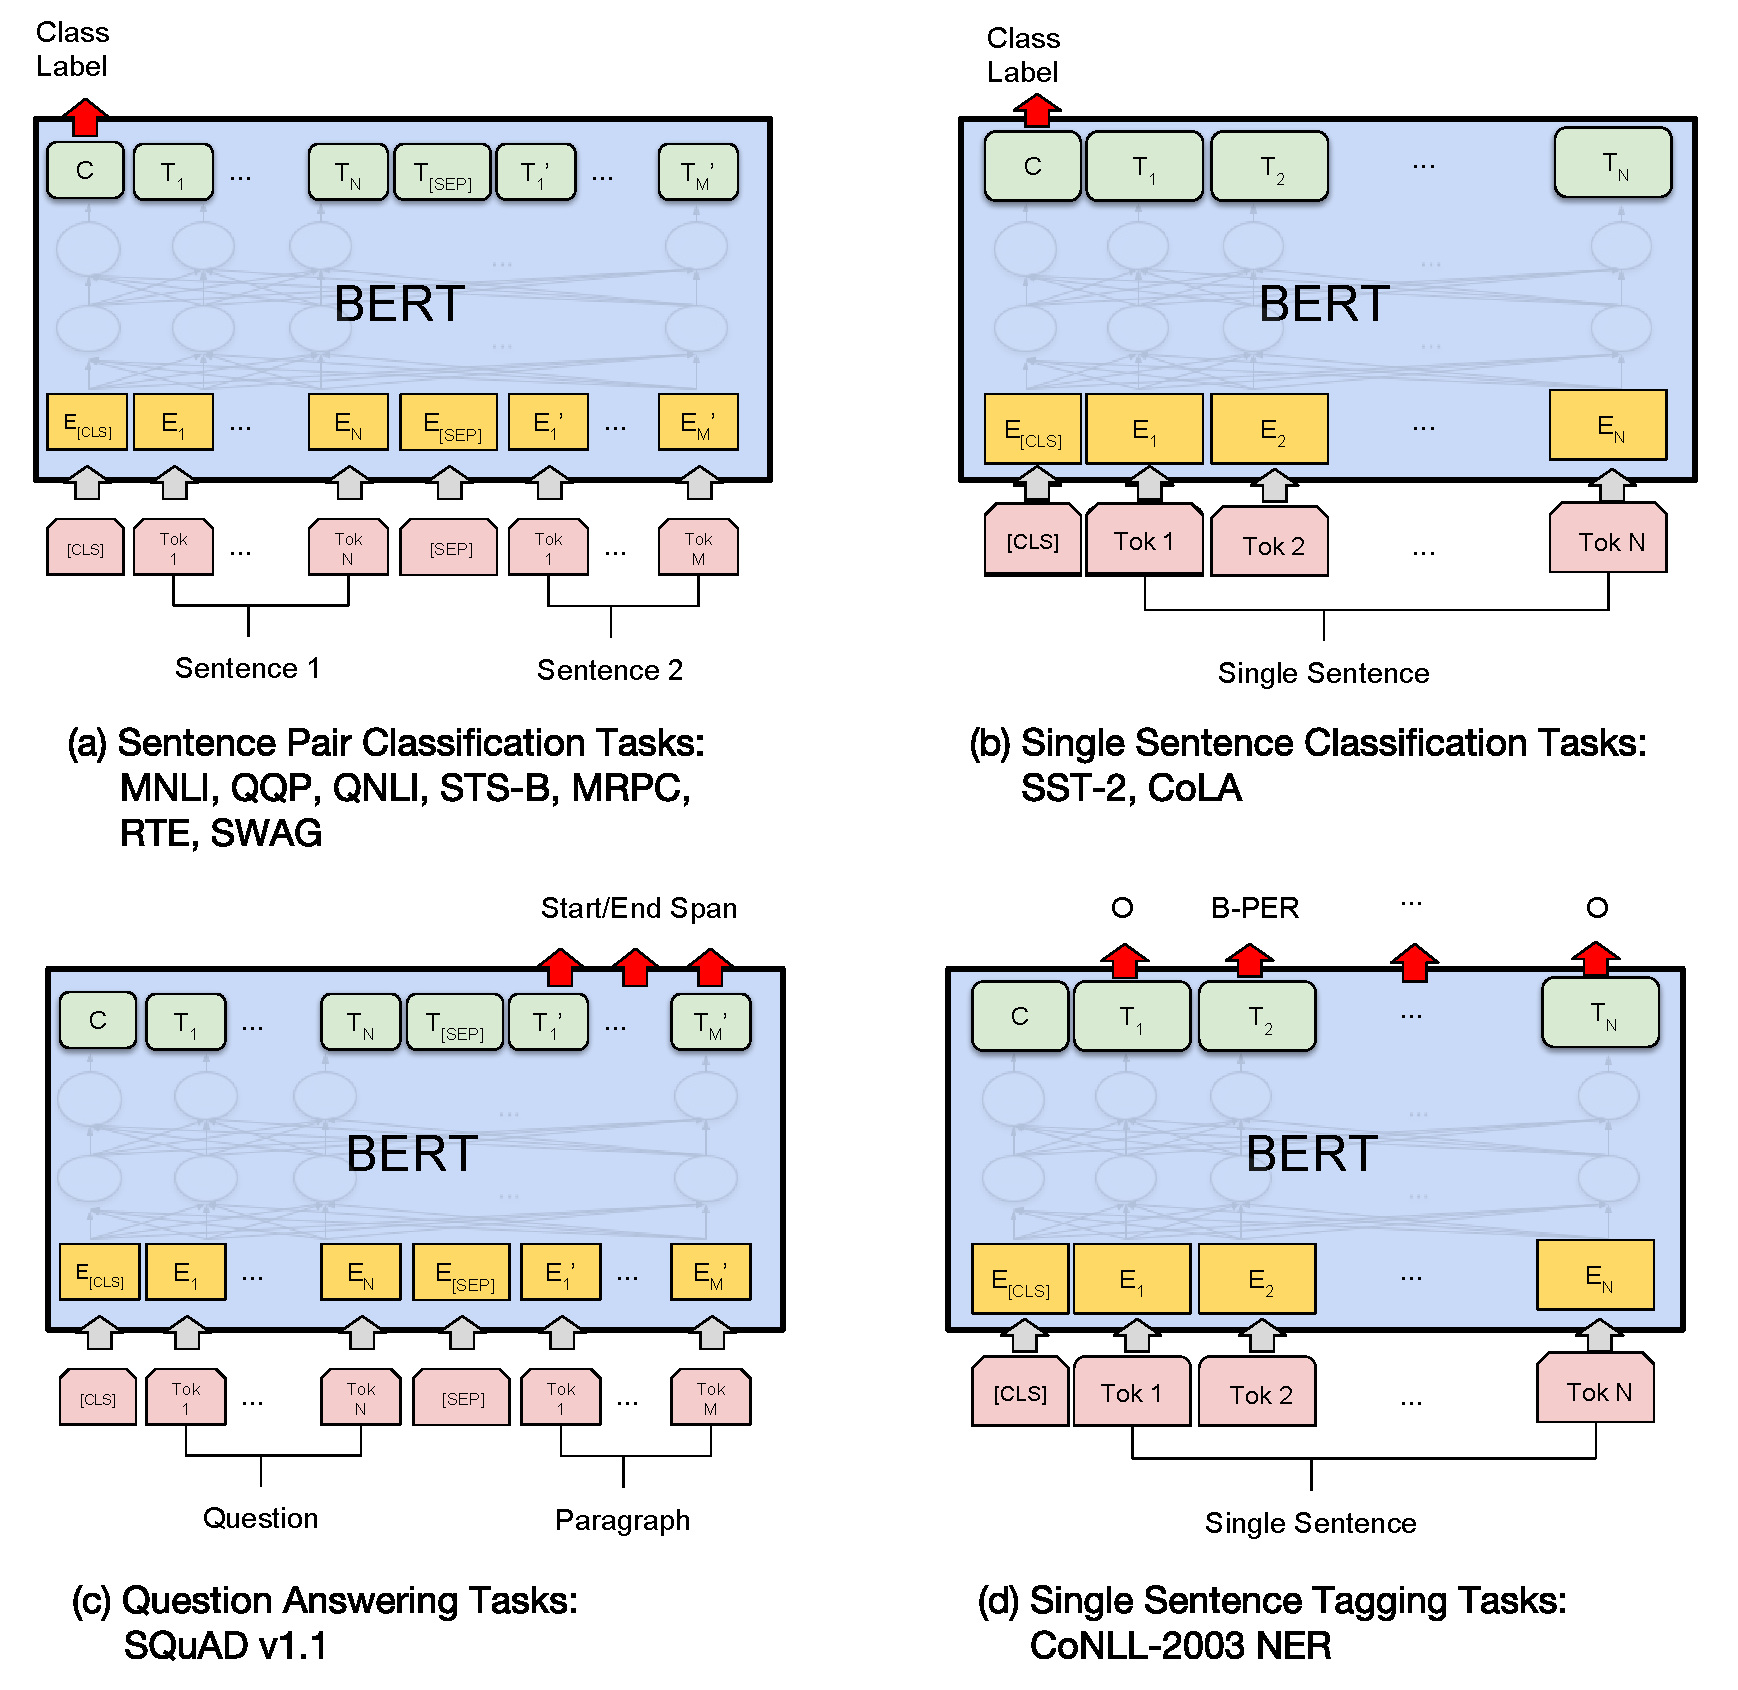
\includegraphics[trim=440 470 0 0, clip,width=1\textwidth]{BERT_fine_tune.pdf}
	\end{center}
\end{figure}

Input:  Single Sentence

Label: Positive (1), negative (0)

Explain:

\begin{center}
	\begin{tabular}{|p{13cm}|p{1cm}|}
		\hline
		Sentence                                                             & label \\
		\hline
		The data shows a significant increase in sales over the last quarter & 1     \\
		\hline
		The research data reveals promising trends in renewable energy usage & 1     \\
		\hline
		The survey data highlights concerns regarding product qualit         & 0     \\
		\hline
		The data reveals a drop in revenue compared to last year             & 0     \\
		\hline
	\end{tabular}
\end{center}

\newpage

\subsection{Fine-tune on the question answering problem}

\begin{figure}[h]
	\begin{center}
		% left bottom right top
		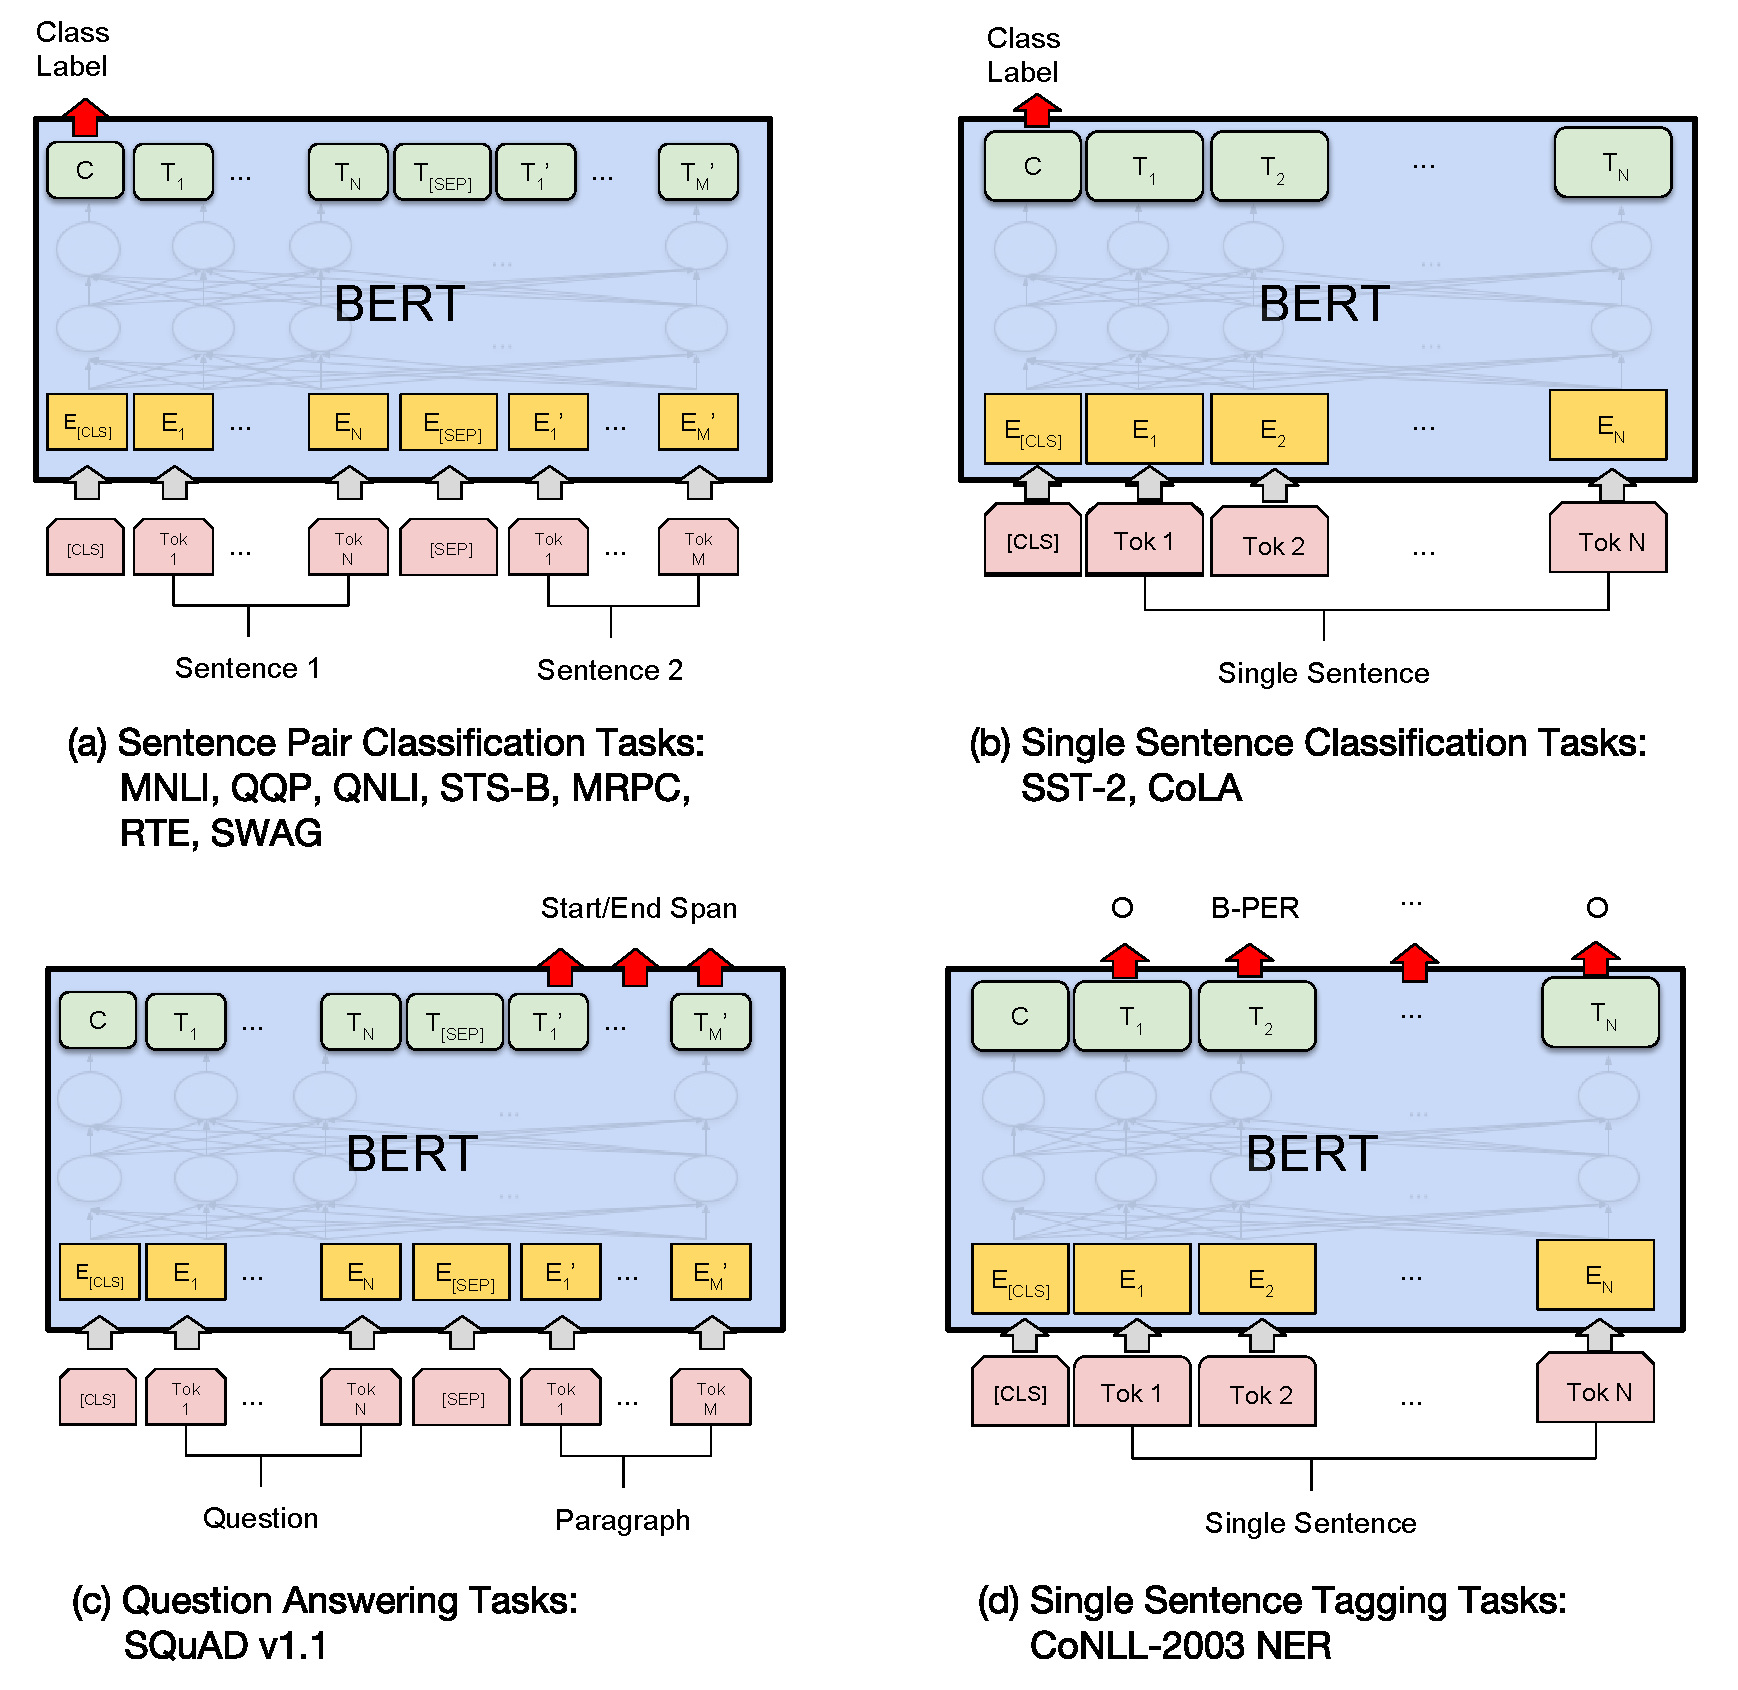
\includegraphics[trim=0 60 440 415, clip,width=1\textwidth]{BERT_fine_tune.pdf}
	\end{center}
\end{figure}
Input:

$\hspace*{0.5cm}$ Question: Lợi ích chính của việc sử dụng nguồn năng lượng tái tạo là gì?

$\hspace*{0.5cm}$ Paragraph: Nguồn năng lượng tái tạo, như năng lượng mặt trời, gió và thủy điện, mang lại nhiều lợi ích chính. Chúng giúp giảm đáng kể khí thải nhà kính, góp phần chống biến đổi khí hậu và cải thiện chất lượng không khí. Ngoài ra, chúng cung cấp giải pháp bền vững lâu dài vì những nguồn này được tái tạo tự nhiên, giảm thiểu sự phụ thuộc vào nhiên liệu hóa thạch có hạn. Hơn nữa, đầu tư vào năng lượng tái tạo tạo ra việc làm trong sản xuất, lắp đặt và bảo trì, thúc đẩy kinh tế địa phương. Cuối cùng, chúng nâng cao an ninh năng lượng bằng cách đa dạng hóa nguồn cung và giảm thiểu rủi ro về biến động giá cả của thị trường nhiên liệu hóa thạch.

Output:

$\hspace*{0.5cm}$ start = 21

$\hspace*{0.5cm}$ end = 43

$\hspace*{0.5cm}$ $\rightarrow$ Answer:Chúng giúp giảm đáng kể khí thải nhà kính, góp phần chống biến đổi khí hậu và cải thiện chất lượng không khí

\newpage

\begin{center}
	\begin{tikzpicture}[
			mynode/.style={draw, text width=0.75cm, align=center, minimum height=0.75cm,line width = 0.5mm}
		]

		\node[align = center,draw, rounded corners=2mm, minimum width=16cm, minimum height=3cm,line width = 0.5mm, fill = blue!30] at (0,1.75) {\textbf{BERT} \\ \textbf{Transformer Encoder}};

		\draw[->, line width = 0.5mm] (-7.5,-1.5) -- (-7.5,0);
		\draw[->, line width = 0.5mm] (-6.5,-1.5) -- (-6.5,0);
		\draw[->, line width = 0.5mm] (-5.5,-1.5) -- (-5.5,0);
		\draw[->, line width = 0.5mm] (-4.5,-1.5) -- (-4.5,0);
		\draw[->, line width = 0.5mm] (-3.5,-1.5) -- (-3.5,0);
		\draw[->, line width = 0.5mm] (-2.5,-1.5) -- (-2.5,0);
		\draw[->, line width = 0.5mm] (-1.5,-1.5) -- (-1.5,0);
		\draw[->, line width = 0.5mm] (-0.5,-1.5) -- (-0.5,0);
		\draw[->, line width = 0.5mm] (0.5,-1.5) -- (0.5,0);
		\draw[->, line width = 0.5mm] (1.5,-1.5) -- (1.5,0);
		\draw[->, line width = 0.5mm] (2.5,-1.5) -- (2.5,0);
		\draw[->, line width = 0.5mm] (3.5,-1.5) -- (3.5,0);
		\draw[->, line width = 0.5mm] (4.5,-1.5) -- (4.5,0);
		\draw[->, line width = 0.5mm] (5.5,-1.5) -- (5.5,0);
		\draw[->, line width = 0.5mm] (6.5,-1.5) -- (6.5,0);
		\draw[->, line width = 0.5mm] (7.5,-1.5) -- (7.5,0);

		\node at (-7.5, -2) {\tiny \textbf{[CLS]}};
		\node[mynode] at (-6.5, -2) {\tiny $Q_1$};
		\node[mynode] at (-5.5, -2) {\tiny $Q_2$};
		\node[mynode] at (-4.5, -2) {\tiny $Q_3$};
		\node[mynode] at (-3.5, -2) {\tiny $Q_4$};
		\node[mynode] at (-2.5, -2) {$\cdots$};
		\node[mynode] at (-1.5, -2) {\tiny $Q_n$};
		\node at (-0.5, -2) {\tiny \textbf{[SEP]}};
		\node[mynode] at (0.5, -2) {\tiny $P_1$};
		\node[mynode] at (1.5, -2) {\tiny $P_2$};
		\node[mynode] at (2.5, -2) {\tiny $P_3$};
		\node[mynode] at (3.5, -2) {\tiny $P_4$};
		\node[mynode] at (4.5, -2) {\tiny $P_5$};
		\node[mynode] at (5.5, -2) {$\cdots$};
		\node[mynode] at (6.5, -2) {\tiny $P_m$};
		\node at (7.5, -2) {\tiny \textbf{[SEP]}};

		\draw[->, line width = 0.5mm] (0.5,3.5) -- (0.5,4.5);
		\draw[->, line width = 0.5mm] (1.5,3.5) -- (1.5,4.5);
		\draw[->, line width = 0.5mm] (2.5,3.5) -- (2.5,4.5);
		\draw[->, line width = 0.5mm] (3.5,3.5) -- (3.5,4.5);
		\draw[->, line width = 0.5mm] (4.5,3.5) -- (4.5,4.5);
		\draw[->, line width = 0.5mm] (5.5,3.5) -- (5.5,4.5);
		\draw[->, line width = 0.5mm] (6.5,3.5) -- (6.5,4.5);

		\node[mynode] at (0.5, 5) {};
		\node[mynode] at (1.5, 5) {};
		\node[mynode] at (2.5, 5) {};
		\node[mynode] at (3.5, 5) {};
		\node[mynode] at (4.5, 5) {};
		\node[mynode] at (5.5, 5) {};
		\node[mynode] at (6.5, 5) {};

		\draw[->, line width = 0.5mm] (0.5,5.5) -- (0.5,6.5);
		\draw[->, line width = 0.5mm] (1.5,5.5) -- (1.5,6.5);
		\draw[->, line width = 0.5mm] (2.5,5.5) -- (2.5,6.5);
		\draw[->, line width = 0.5mm] (3.5,5.5) -- (3.5,6.5);
		\draw[->, line width = 0.5mm] (4.5,5.5) -- (4.5,6.5);
		\draw[->, line width = 0.5mm] (5.5,5.5) -- (5.5,6.5);
		\draw[->, line width = 0.5mm] (6.5,5.5) -- (6.5,6.5);

		\node[align = center,draw, rounded corners=2mm, minimum width=7.2cm, minimum height=3cm,line width = 0.5mm, fill = green!30] at (3.5,8.2) {Learn token start(end) \\ linear};

		\draw[->, line width = 0.5mm] (0.5,10) -- (0.5,11);
		\draw[->, line width = 0.5mm] (1.5,10) -- (1.5,11);
		\draw[->, line width = 0.5mm] (2.5,10) -- (2.5,11);
		\draw[->, line width = 0.5mm] (3.5,10) -- (3.5,11);
		\draw[->, line width = 0.5mm] (4.5,10) -- (4.5,11);
		\draw[->, line width = 0.5mm] (5.5,10) -- (5.5,11);
		\draw[->, line width = 0.5mm] (6.5,10) -- (6.5,11);

		\node[align = center,draw, rounded corners=2mm, minimum width=7.2cm, minimum height=1.5cm,line width = 0.5mm, fill = red!30] at (3.5,12) {Softmax};

		\draw[->, line width = 0.5mm] (0.5,13) -- (0.5,14);
		\draw[->, line width = 0.5mm] (1.5,13) -- (1.5,14);
		\draw[->, line width = 0.5mm] (2.5,13) -- (2.5,14);
		\draw[->, line width = 0.5mm] (3.5,13) -- (3.5,14);
		\draw[->, line width = 0.5mm] (4.5,13) -- (4.5,14);
		\draw[->, line width = 0.5mm] (5.5,13) -- (5.5,14);
		\draw[->, line width = 0.5mm] (6.5,13) -- (6.5,14);

		\node[mynode] at (0.5, 14.5) {\tiny \textbf{0.1}};
		\node[mynode] at (1.5, 14.5) {\tiny \textbf{0.05}};
		\node[mynode] at (2.5, 14.5) {\tiny \textbf{0.3}};
		\node[mynode] at (3.5, 14.5) {\tiny \textbf{0.09}};
		\node[mynode] at (4.5, 14.5) {\tiny \textbf{0.04}};
		\node[mynode] at (5.5, 14.5) {$\cdots$};
		\node[mynode] at (6.5, 14.5) {\tiny \textbf{0.2}};

	\end{tikzpicture}
\end{center}


\newpage

\subsection{Fine-tune on the token classification problem}

\begin{figure}[h]
	\begin{center}
		% left bottom right top
		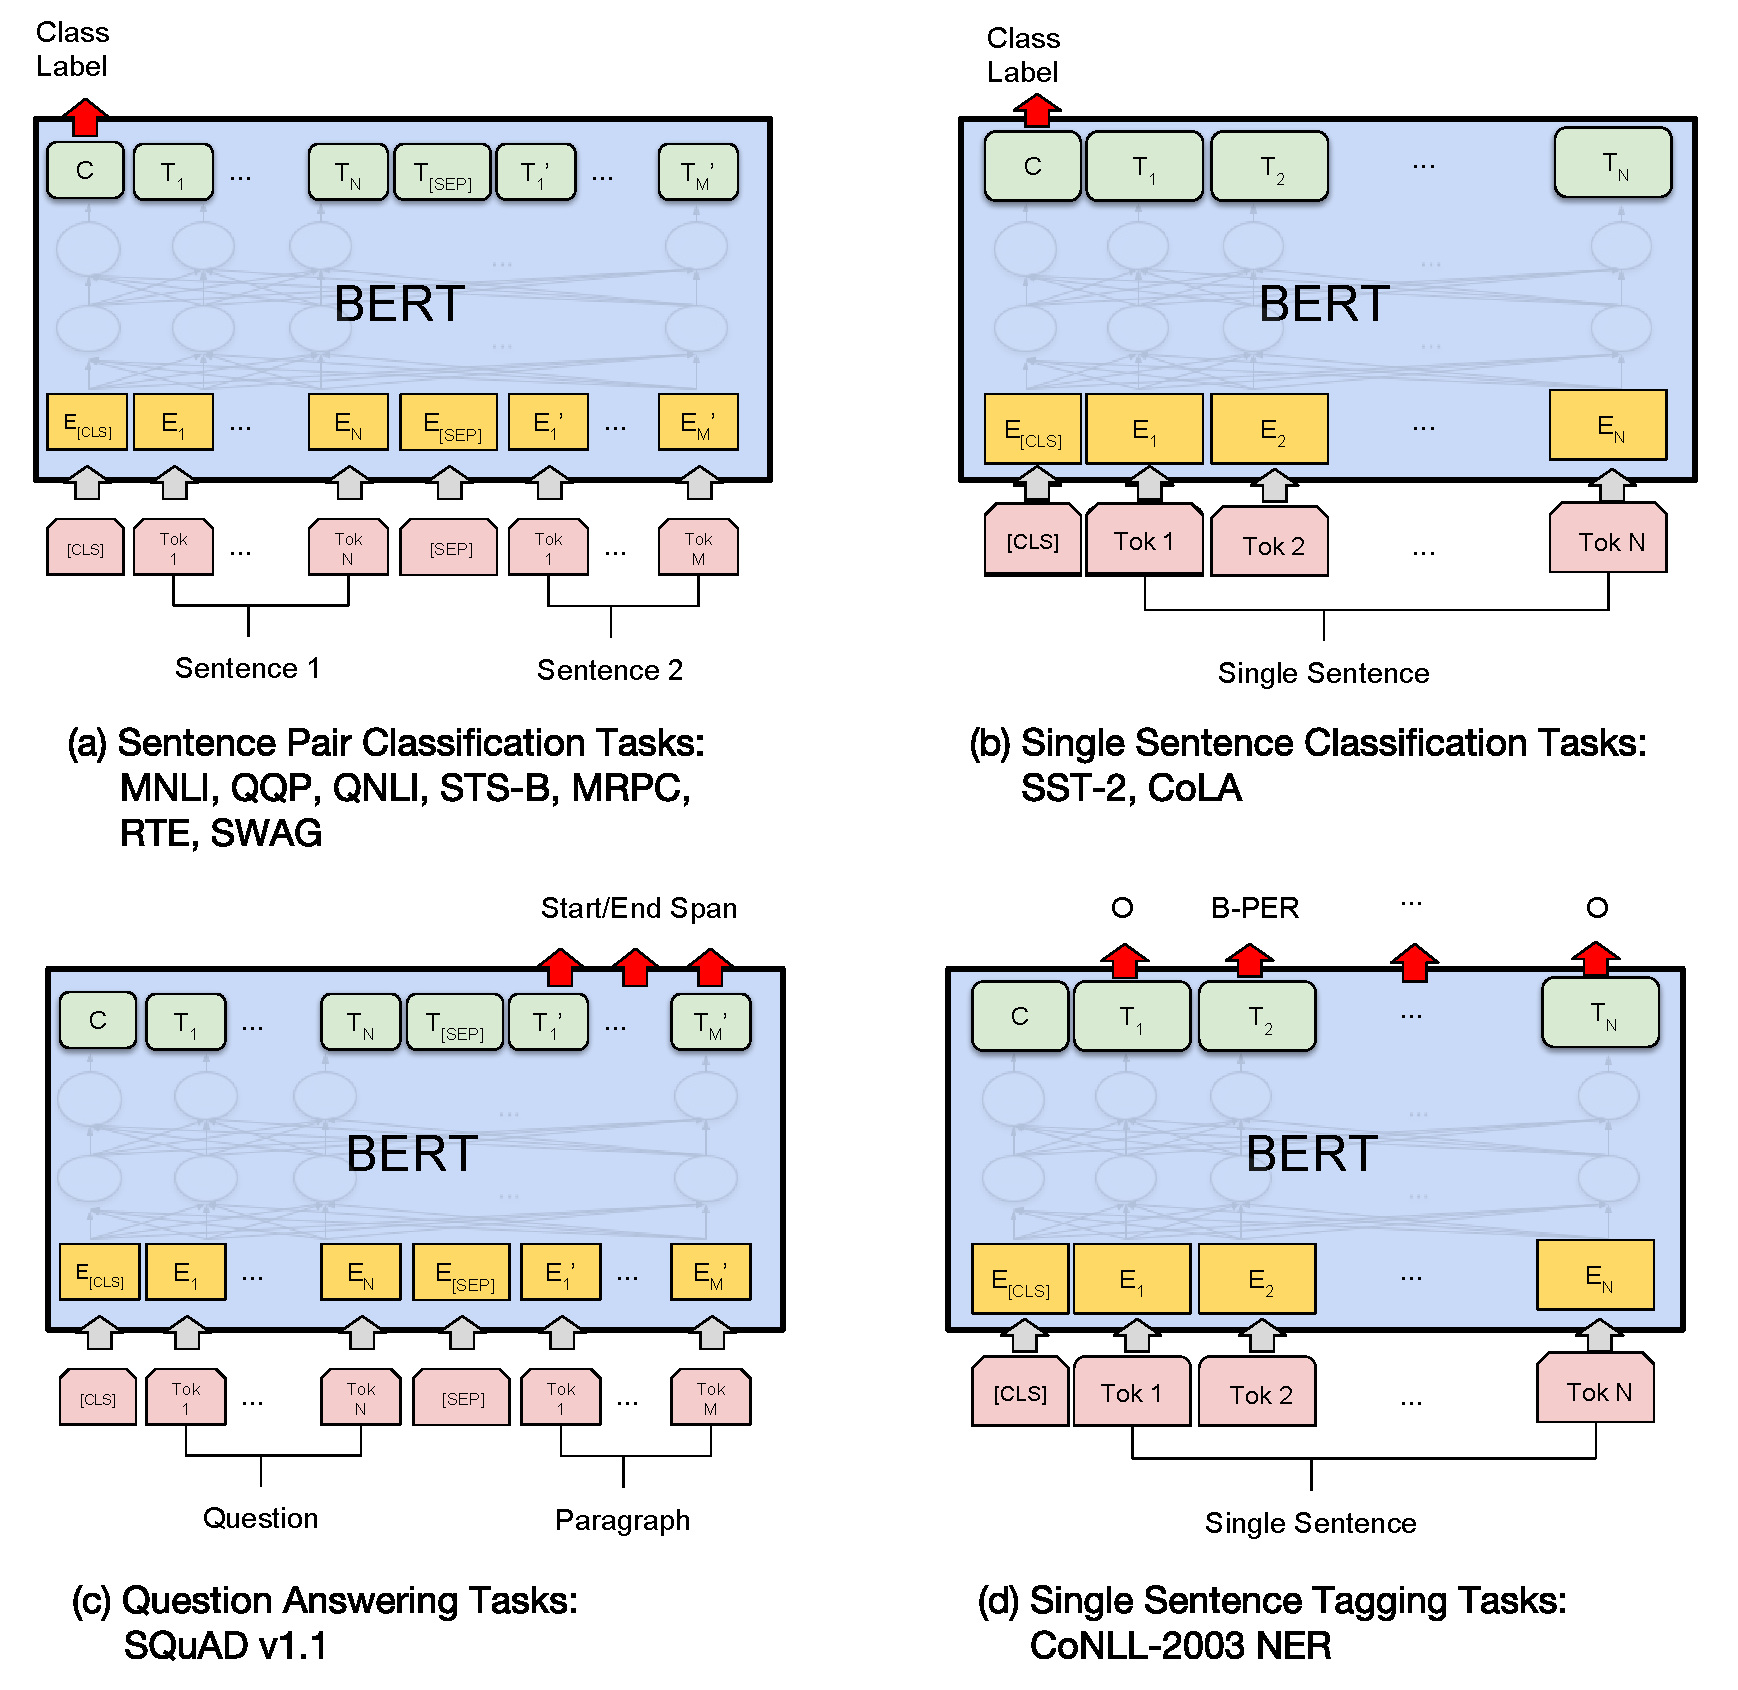
\includegraphics[trim=400 60 0 400, clip,width=1\textwidth]{BERT_fine_tune.pdf}
	\end{center}
\end{figure}

Bài toán nhận diện POS Tag (Post-of-speech tagging)

Bài toán nhận diện thực thể NER(Named Entity Recognition):

Example:

Input:

$\hspace*{0.5cm}$ [CLS] The capital of Viet Nam is Ha Noi [SEP].

Output:

$\hspace*{0.5cm}$ o o o B-location I-loction o B-location I-location.

Explain:

$\hspace*{0.5cm}$ o: outside name entity

$\hspace*{0.5cm}$Với mỗi entity kiểu T, ta có hai nhãn B-T và I-T. B-T là begin type T, I-T là inside type T.

\newpage

\chapter{T5(The Text-To-Text Transfer Transformer)}

\chapter{Transformer Avanced}

\chapter{SMT Statitic Machine Translate}

\chapter{LLM Large Language Models}


\part{Application}
\setcounter{chapter}{0}


\chapter{ Truy vấn thông tin (Information Retrieval)}

\chapter{RAG (Retrieval Augmented Generation)}

\chapter{AI Agent}

\section{Reinforcement Learning }

\begin{center}
	\begin{tikzpicture}
		\node[draw=blue, fill=gray!20, rounded corners=2mm, minimum width=3cm, minimum height=2cm, line width=0.5mm] at (0,0) {\textbf{Agent}};
		\node[draw=blue, fill=gray!20, rounded corners=2mm, minimum width=3cm, minimum height=2cm, line width=0.5mm] at (8,0) {\textbf{Enviroment}};

		\draw[<-, line width = 0.75mm, color = red]   (1.5,-0.5) -- (6.5,-0.5);
		\draw[->, line width = 0.75mm, color = red]   (1.5,0.5) -- (6.5,0.5);

		\node at (3.75,0.75) {\textbf{Action}};
		\node at (3.75,-0.75) {\textbf{Observation}};
	\end{tikzpicture}
\end{center}

\begin{itemize}
	\item Agent tương tác với môi trường và nhân về các observation.
	\item Ví dụ: Agent làm sai sẽ bị phạt, Agent làm đúng sẽ được cộng điểm.
\end{itemize}

\section{React}

\textbf{React = Reason + action}

\begin{itemize}
	\item	React là một Framework giúp các tác nhân (Agents) giải quyết vấn đề một cách hiệu quả bằng cách kết hợp Lý luận(Reason) và hành động(Act) theo từng bước.
\end{itemize}

\begin{center}
	\begin{tikzpicture}
		\node[draw=blue, fill=gray!20, rounded corners=3mm, minimum width=3cm, minimum height=2cm, line width=0.5mm] at (0,6) {\textbf{Reason}};
		\node[draw=blue, fill=gray!20, rounded corners=3mm, minimum width=3cm, minimum height=2cm, line width=0.5mm] at (0,3) {\textbf{Action}};
		\node[draw=blue, fill=gray!20, rounded corners=3mm, minimum width=3cm, minimum height=2cm, line width=0.5mm] at (0,0) {\textbf{Observation}};

		\draw[->, line width = 0.5mm, color = red] (0,5) --(0,4);
		\draw[->, line width = 0.5mm, color = red] (0,2) -- (0,1);

		\draw[line width = 0.5mm, color = red] (1.5,0) -- (2.5,0);
		\draw[line width = 0.5mm, color = red] (2.5,0) -- (2.5,6);
		\draw[->,line width = 0.5mm, color = red] (2.5,6) -- (1.5,6);

	\end{tikzpicture}
\end{center}

\begin{itemize}
	\item Tác nhân suy nghĩ logic để đưa ra các giả định hoặc phán đoán đựa trên thông tin hiện có. Lý luận này dựa vào các bước phân tích vấn để để tìm ra hướng giải quyết phù hợp.
	\item Sau mỗi bước suy nghĩ, tác nhân thực hiện một hành động cụ thể. Hành động này cung cấp thêm thông tin hoặc giải pháp để tiến tới bước tiếp theo.
	\item Mỗi hành động thực hiện sẽ mang lại kết quả hoặc phản hồi. Kết quả này được sử dụng để bổ sung vào quá trình lý luận cho các bước tiếp theo.
	\item Chu trình Lý luận $\Rightarrow$ hành động $\Rightarrow$ Quan sát được lặp lại cho đến khi đặt được mục tiêu cuối cùng. Tác nhân không dừng lại cho đến khi tìm được câu trả lời hoặc giải pháp thỏa đáng.
\end{itemize}

Một ví dụ nhỏ để hình dung được:


\begin{center}
	\begin{tikzpicture}
		\node[align=center, draw=blue, fill=gray!20, rounded corners=3mm, minimum height=1.5cm, text width=10cm, line width=0.5mm] at (0,10) {
			\textbf{User}: Bring me a coffee
		};
		\node[align=center, draw=blue, fill=gray!20, rounded corners=3mm, minimum height=1.5cm, text width=10cm, line width=0.5mm] at (0,8) {
			\textbf{Thought}: To make coffee, I need a coffee machine and Arabica ground coffee.
		};
		\node[align=center, draw=blue, fill=gray!20, rounded corners=3mm, minimum height=1.5cm, text width=10cm, line width=0.5mm] at (0,6) {
			\textbf{Action}: ToolSelection(tool="coffee machine", ingredient="Arabica ground coffee")
		};
		\node[align=center, draw=blue, fill=gray!20, rounded corners=3mm, minimum height=1.5cm, text width=10cm, line width=0.5mm] at (0,4) {
			\textbf{Observation}: Coffee machine and ingredients have been selected.
		};
		\node[align=center, draw=blue, fill=gray!20, rounded corners=3mm, minimum height=1.5cm, text width=10cm, line width=0.5mm] at (0,2) {
			\textbf{Thought}: Start brewing coffee with the selected machine.
		};
		\node[align=center, draw=blue, fill=gray!20, rounded corners=3mm, minimum height=1.5cm, text width=10cm, line width=0.5mm] at (0,0) {
			\textbf{Action}: BrewCoffee(tool="coffee machine", ingredient="Arabica ground coffee", water="hot")
		};
		\node[align=center, draw=blue, fill=gray!20, rounded corners=3mm, minimum height=1.5cm, text width=10cm, line width=0.5mm] at (0,-2) {
			\textbf{Observation}: Coffee has been brewed.
		};
		\node[align=center, draw=blue, fill=gray!20, rounded corners=3mm, minimum height=1.5cm, text width=10cm, line width=0.5mm] at (0,-4) {
			\textbf{Final Answer}: Coffee is ready.
		};

		\draw[->, color = red, line width = 0.5mm] (-4,9.25) -- (-4,8.75);
		\draw[->, color = red, line width = 0.5mm] (-3,9.25) -- (-3,8.75);
		\draw[->, color = red, line width = 0.5mm] (-2,9.25) -- (-2,8.75);
		\draw[->, color = red, line width = 0.5mm] (-1,9.25) -- (-1,8.75);
		\draw[->, color = red, line width = 0.5mm] (0,9.25) -- (0,8.75);
		\draw[->, color = red, line width = 0.5mm] (1,9.25) -- (1,8.75);
		\draw[->, color = red, line width = 0.5mm] (2,9.25) -- (2,8.75);
		\draw[->, color = red, line width = 0.5mm] (3,9.25) -- (3,8.75);
		\draw[->, color = red, line width = 0.5mm] (4,9.25) -- (4,8.75);


		\draw[->, color = red, line width = 0.5mm] (-4,7.25) -- (-4,6.75);
		\draw[->, color = red, line width = 0.5mm] (-3,7.25) -- (-3,6.75);
		\draw[->, color = red, line width = 0.5mm] (-2,7.25) -- (-2,6.75);
		\draw[->, color = red, line width = 0.5mm] (-1,7.25) -- (-1,6.75);
		\draw[->, color = red, line width = 0.5mm] (0,7.25) -- (0,6.75);
		\draw[->, color = red, line width = 0.5mm] (1,7.25) -- (1,6.75);
		\draw[->, color = red, line width = 0.5mm] (2,7.25) -- (2,6.75);
		\draw[->, color = red, line width = 0.5mm] (3,7.25) -- (3,6.75);
		\draw[->, color = red, line width = 0.5mm] (4,7.25) -- (4,6.75);


		\draw[->, color = red, line width = 0.5mm] (-4,5.25) -- (-4,4.75);
		\draw[->, color = red, line width = 0.5mm] (-3,5.25) -- (-3,4.75);
		\draw[->, color = red, line width = 0.5mm] (-2,5.25) -- (-2,4.75);
		\draw[->, color = red, line width = 0.5mm] (-1,5.25) -- (-1,4.75);
		\draw[->, color = red, line width = 0.5mm] (0,5.25) -- (0,4.75);
		\draw[->, color = red, line width = 0.5mm] (1,5.25) -- (1,4.75);
		\draw[->, color = red, line width = 0.5mm] (2,5.25) -- (2,4.75);
		\draw[->, color = red, line width = 0.5mm] (3,5.25) -- (3,4.75);
		\draw[->, color = red, line width = 0.5mm] (4,5.25) -- (4,4.75);


		\draw[->, color = red, line width = 0.5mm] (-4,3.25) -- (-4,2.75);
		\draw[->, color = red, line width = 0.5mm] (-3,3.25) -- (-3,2.75);
		\draw[->, color = red, line width = 0.5mm] (-2,3.25) -- (-2,2.75);
		\draw[->, color = red, line width = 0.5mm] (-1,3.25) -- (-1,2.75);
		\draw[->, color = red, line width = 0.5mm] (0,3.25) -- (0,2.75);
		\draw[->, color = red, line width = 0.5mm] (1,3.25) -- (1,2.75);
		\draw[->, color = red, line width = 0.5mm] (2,3.25) -- (2,2.75);
		\draw[->, color = red, line width = 0.5mm] (3,3.25) -- (3,2.75);
		\draw[->, color = red, line width = 0.5mm] (4,3.25) -- (4,2.75);


		\draw[->, color = red, line width = 0.5mm] (-4,1.25) -- (-4,0.75);
		\draw[->, color = red, line width = 0.5mm] (-3,1.25) -- (-3,0.75);
		\draw[->, color = red, line width = 0.5mm] (-2,1.25) -- (-2,0.75);
		\draw[->, color = red, line width = 0.5mm] (-1,1.25) -- (-1,0.75);
		\draw[->, color = red, line width = 0.5mm] (0,1.25) -- (0,0.75);
		\draw[->, color = red, line width = 0.5mm] (1,1.25) -- (1,0.75);
		\draw[->, color = red, line width = 0.5mm] (2,1.25) -- (2,0.75);
		\draw[->, color = red, line width = 0.5mm] (3,1.25) -- (3,0.75);
		\draw[->, color = red, line width = 0.5mm] (4,1.25) -- (4,0.75);


		\draw[->, color = red, line width = 0.5mm] (-4,-0.75) -- (-4,-1.25);
		\draw[->, color = red, line width = 0.5mm] (-3,-0.75) -- (-3,-1.25);
		\draw[->, color = red, line width = 0.5mm] (-2,-0.75) -- (-2,-1.25);
		\draw[->, color = red, line width = 0.5mm] (-1,-0.75) -- (-1,-1.25);
		\draw[->, color = red, line width = 0.5mm] (0,-0.75) -- (0,-1.25);
		\draw[->, color = red, line width = 0.5mm] (1,-0.75) -- (1,-1.25);
		\draw[->, color = red, line width = 0.5mm] (2,-0.75) -- (2,-1.25);
		\draw[->, color = red, line width = 0.5mm] (3,-0.75) -- (3,-1.25);
		\draw[->, color = red, line width = 0.5mm] (4,-0.75) -- (4,-1.25);


		\draw[->, color = red, line width = 0.5mm] (-4,-2.75) -- (-4,-3.25);
		\draw[->, color = red, line width = 0.5mm] (-3,-2.75) -- (-3,-3.25);
		\draw[->, color = red, line width = 0.5mm] (-2,-2.75) -- (-2,-3.25);
		\draw[->, color = red, line width = 0.5mm] (-1,-2.75) -- (-1,-3.25);
		\draw[->, color = red, line width = 0.5mm] (0,-2.75) -- (0,-3.25);
		\draw[->, color = red, line width = 0.5mm] (1,-2.75) -- (1,-3.25);
		\draw[->, color = red, line width = 0.5mm] (2,-2.75) -- (2,-3.25);
		\draw[->, color = red, line width = 0.5mm] (3,-2.75) -- (3,-3.25);
		\draw[->, color = red, line width = 0.5mm] (4,-2.75) -- (4,-3.25);



		\draw[->, color = red, line width = 0.5mm] (0,-0.75) -- (0,-1.25);

		\draw[->, color = red, line width = 0.5mm] (0,-2.75) -- (0,-3.25);
	\end{tikzpicture}
\end{center}

\section{Prompt}

\subsection{Prompt Element}

\begin{itemize}
	\item Yêu cầu (Instruction): rõ ràng, xúc tích.
	\item Ngữ cảnh (Context): đầy đủ thông tin.
	\item Dữ liệu đầu vào (Input Data)
	\item Định dạng đầu ra (Output Indicator): chặt chẽ để tương thích với ứng dụng(ví dụ csv, json, $\dots$)
\end{itemize}


$\ast$ \textbf{Tip:} Thêm \#\#\#  ví dụ: \#\#\# Yêu cầu \#\#\#  $\rightarrow$ khớp với mô hình được đào tạo.


\section{Funtion calling}

\begin{itemize}
	\item Gọi hàm (Function Calling) cho phép các Mô hình Ngôn ngữ Lớn (LLMs) tương tác với các công cụ, API và hàm bên ngoài dựa trên đầu vào của người dùng. Thay vì chỉ tạo ra văn bản thuần túy, LLM có thể nhận biết khi nào cần thực hiện một hành động cụ thể và sau đó yêu cầu một hàm bên ngoài xử lý tác vụ đó.

	\item Với khả năng này, người dùng có thể tương tác với các hệ thống phức tạp chỉ bằng ngôn ngữ tự nhiên, trong khi LLM đảm nhiệm việc thực thi các chức năng nền tảng. Điều này giúp mô hình không chỉ tạo ra nội dung mà còn giải quyết các vấn đề thực tế một cách hiệu quả.

	\item Ví dụ, nếu người dùng hỏi về thời tiết, thay vì chỉ trả lời chung chung, mô hình có thể gọi API thời tiết để lấy dữ liệu theo thời gian thực. Hơn thế nữa, nếu dự báo có mưa, LLM thậm chí có thể nhắc bạn mang theo ô khi ra ngoài, giúp trải nghiệm tương tác trở nên thông minh và hữu ích hơn.
\end{itemize}a

\newpage

How Function Calling Works:

\begin{center}
	\begin{tikzpicture}
		\node[align=center, draw=gray, fill=gray!20, rounded corners=1mm, minimum height=1.5cm, text width=3cm, line width=0.5mm] at (0,0) {
			\textbf{User Query}
		};

		\node[align=center, draw=blue, fill=gray!20, circle , minimum size=2.5cm] at (5,0) {
			\large\color{blue}\textbf{LLMs}
		};

		\node[draw=ForestGreen, thick, fill=gray!20, diamond, minimum size=2cm, align=center] at (10,0) {
			\color{ForestGreen}\textbf{Function}
			\\
			\color{ForestGreen}\textbf{Call}
		};


		\node[align=center, draw=orange, fill=gray!20, circle , minimum size=2.25cm] at (10,4) {
			\color{orange}\textbf{Custom}
			\\
			\color{orange}\textbf{Function}
		};

		\node[align=center, draw=red, fill=gray!20, circle , minimum size=2.25cm] at (10,-4) {
			\color{red}\textbf{API}

		};


		\draw[->, color = red, line width = 0.5mm, dashed] (1.7,0.25) -- (3.75,0.25);
		\draw[<-, color = red, line width = 0.5mm, dashed] (1.7,-0.25) -- (3.75,-0.25);

		\draw[->, color = red, line width = 0.5mm, dashed] (6.25,0.25) -- (8.7,0.25);
		\draw[<-, color = red, line width = 0.5mm, dashed] (6.25,-0.25) -- (8.7,-0.25);

		\draw[->, color = red, line width = 0.5mm, dashed] (9.75,1.45) -- (9.75,2.75);
		\draw[<-, color = red, line width = 0.5mm, dashed] (10.25,1.45) -- (10.25,2.75);

		\draw[->, color = red, line width = 0.5mm, dashed] (9.75,-1.3) -- (9.75,-2.85);
		\draw[<-, color = red, line width = 0.5mm, dashed] (10.25,-1.3) -- (10.25,-2.85);



	\end{tikzpicture}
\end{center}


\begin{itemize}
	\item \textbf{Truy vấn của người dùng (User Query)}: Quá trình bắt đầu khi người dùng đặt câu hỏi hoặc yêu cầu một hành động (ví dụ: "Có những khách hàng tiềm năng nào trong CRM của tôi?" hoặc "Kiểm tra xem sản phẩm X còn hàng không").

	\item \textbf{Xử lý bởi LLM (LLM Processing)}: LLM phân tích truy vấn và nhận ra rằng cần có dữ liệu bên ngoài hoặc hành động cụ thể để đáp ứng yêu cầu. Ví dụ:
	      \begin{itemize}
		      \item Nếu người dùng hỏi về khách hàng tiềm năng trong CRM, LLM xác định rằng cần lấy dữ liệu thời gian thực.
		      \item Nếu người dùng muốn kiểm tra tồn kho sản phẩm, LLM sẽ kích hoạt một truy vấn vào cơ sở dữ liệu.
	      \end{itemize}

	\item \textbf{Quyết định gọi hàm (Function Call Decision)}: LLM quyết định thực hiện một lệnh gọi hàm, có thể là:
	      \begin{itemize}
		      \item \textbf{Gọi API (API Calls)}: Kết nối với các dịch vụ bên ngoài (ví dụ: API của CRM để lấy dữ liệu khách hàng tiềm năng theo thời gian thực từ Salesforce).
		      \item \textbf{Hàm tùy chỉnh (Custom Functions)}: Truy cập vào các công cụ hoặc cơ sở dữ liệu nội bộ (ví dụ: Kiểm tra mức tồn kho trong hệ thống quản lý kho).
	      \end{itemize}

	\item \textbf{Truy xuất dữ liệu (Data Retrieval)}: Hàm được gọi sẽ tìm nạp dữ liệu cần thiết (ví dụ: danh sách khách hàng tiềm năng từ API của Salesforce hoặc thông tin tồn kho từ cơ sở dữ liệu kho hàng).

	\item \textbf{Tích hợp dữ liệu (Data Integration)}: Dữ liệu thu thập được gửi lại cho LLM, sau đó mô hình xử lý và tạo ra một phản hồi có ngữ cảnh và chính xác cho người dùng.
\end{itemize}

\newpage

Example of how it works:

\textbf{Step 1}: Define available functions (schemas for LLM)

\begin{lstlisting}
function_definitions = [
	{
		"name": "book_flight",
		"description": "Book a flight ticket between two cities",
		"parameters": {
			"type": "object",
			"properties": {
				"from_city": {
					"type": "string",
					"description": "Departure city"
				},
				"to_city": {
					"type": "string",
					"description": "Destination city"
				},
				"date": {
					"type": "string",
					"description": "Flight date in YYYY-MM-DD format"
				}
			},
			"required": ["from_city", "to_city", "date"]
		}
	}
]
	\end{lstlisting}


\textbf{Step 2}: User query input

\begin{lstlisting}
user_query = "Book a flight from New York to Los Angeles on March 15."
	\end{lstlisting}

\textbf{Step 3}: Simulate LLM extracting function\_call output
In real use, GPT-4,OPEN AI, LLama, Gemini,etc would return this automatically
\begin{lstlisting}
function_call = {
	"name": "book_flight",
	"arguments": {
		"from_city": "New York",
		"to_city": "Los Angeles",
		"date": "2025-03-15"
	}
}
\end{lstlisting}


\textbf{Step 4}: Define the actual function to be called

\begin{lstlisting}
def book_flight(from_city, to_city, date):
	return f"Flight booked from {from_city} to {to_city} on {date}."
\end{lstlisting}

\newpage

\textbf{Step 5}: Execute the function using parsed arguments from LLM

\begin{lstlisting}
if function_call["name"] == "book_flight":
	result = book_flight(**function_call["arguments"])
	print(result)
\end{lstlisting}

\textbf{Result}:


\begin{lstlisting}[backgroundcolor=\color{black}, basicstyle=\color{white}\ttfamily]
	Flight booked from New York to Los Angeles on 2025-03-15.
	\end{lstlisting}

Có thể sinh trực tiếp function\textunderscore definitions tại \href{https://platform.openai.com/playground/prompts?models=gpt-4o}{OPEN AI Prompts}

\section{Định nghĩa về AI Agent}

AI Agent là sự kết hợp chặt chẽ giữa các thành phần như lý luận (Reason), hành động (Action), phản hồi (Observation), và khả năng gọi hàm (Function Calling) để thực thi nhiệm vụ một cách tự động và thông minh.

\begin{itemize}
    \item AI Agent hoạt động theo một chu trình lặp gồm: Lý luận $\Rightarrow$ Hành động $\Rightarrow$ Quan sát, tương tự như mô hình React đã trình bày ở phần trước.
    
    \item Trong mỗi bước hành động, AI Agent có thể thực hiện Function Calling — gọi đến các hàm hoặc API bên ngoài để thu thập dữ liệu, thực hiện tác vụ hoặc truy xuất kết quả.

    \item Việc sử dụng Function Calling giúp AI Agent không chỉ xử lý logic nội tại, mà còn tương tác hiệu quả với môi trường bên ngoài (như hệ thống dữ liệu, công cụ hỗ trợ, hoặc API).

    \item Các function được gọi có thể là: 
    \begin{itemize}
        \item API từ hệ thống bên ngoài (ví dụ: tra cứu thời tiết, thông tin kho hàng).
        \item Hàm tùy chỉnh trong hệ thống nội bộ (ví dụ: xử lý CRM, báo cáo doanh thu).
    \end{itemize}

    \item AI Agent thường được xây dựng dưới dạng một hệ thống có khả năng:
    \begin{itemize}
        \item \textbf{Lập kế hoạch (Planner)}: xác định các bước cần thực hiện để hoàn thành mục tiêu.
        \item \textbf{Thực thi (Executor)}: gọi các hàm tương ứng để xử lý từng bước.
        \item \textbf{Ghi nhớ (Memory)}: lưu thông tin, quan sát và kết quả phục vụ cho các bước sau.
        \item \textbf{Lặp lại (Loop)}: tiếp tục quá trình suy nghĩ – hành động – quan sát cho đến khi đạt mục tiêu cuối cùng.
    \end{itemize}
    
    \item Nhờ đó, AI Agent có khả năng tự động hóa quy trình, ra quyết định thông minh và phản ứng linh hoạt trước nhiều tình huống phức tạp trong thế giới thực.
\end{itemize}

% ngu thật
\end{document}
